\documentclass[11pt]{report}
\usepackage{graphicx}
\usepackage[margin = 2.5cm]{geometry}
\usepackage[T1]{fontenc}
\usepackage{setspace}
\usepackage{tikz}
\usepackage{amsmath}
\usepackage{amssymb}
\usepackage{verbatim}
\usepackage{lscape}
\usepackage{mdframed}
\usepackage{xcolor}

% checkmarks
\def\checkmark{\tikz\fill[scale=0.4](0,.35) -- (.25,0) -- (1,.7) -- (.25,.15) -- cycle;} 

% fancy chapter headers
\usepackage{titlesec, blindtext, color}
\definecolor{gray75}{gray}{0.75}
\newcommand{\hsp}{\hspace{20pt}}
\titleformat{\chapter}[hang]{\Huge\bfseries}{\thechapter\hsp\textcolor{gray75}{|}\hsp}{0pt}{\Huge\bfseries}

% captions
\usepackage[labelfont=bf]{caption}
\captionsetup{skip=7pt, font=footnotesize} %,font={stretch=1}

% tables
\usepackage{multirow}
%\usepackage{longtable} 
\usepackage{array}
%\usepackage{verbatim} 
\usepackage{csvsimple}

% clinkable links 
\usepackage[hidelinks]{hyperref}
\hypersetup{
    colorlinks=false, %set true if you want colored links
    linktoc=all     %set to all if you want both sections and subsections linked
    %linkcolor=blue,  %choose some color if you want links to stand out
}

% Bibliography
\usepackage[backend=bibtex, natbib=true, url=false, doi=true, isbn=false, style=authoryear-comp, eprint=false, maxbibnames= 20, firstinits=true, maxcitenames=2]{biblatex}
\addbibresource{LIBRARY.bib}
% remove "" around title
\DeclareFieldFormat
  [article,inbook,incollection,inproceedings,patent,thesis,unpublished]
  {title}{#1\isdot}
% author: last name, first name
\DeclareNameAlias{sortname}{last-first}
% remove pp before pages
\DeclareFieldFormat{pages}{#1}
% remove comma / space before pages, and put colon instead
%\renewcommand*{\bibpagespunct}{%
%\ifentrytype{article}
%  {\addcolon}
% {\addcomma\space}}
% remove 'in:'
\renewbibmacro{in:}{}
% remove point after volume number, and issue number
\renewbibmacro*{volume+number+eid}{%
  \printfield{volume}%
  \setunit*{\adddot}% DELETED (point)
  \printfield{number}% DELETED (issue number)
  \setunit{\addcomma\space}% DELETED
  \printfield{eid} % DELETED
  }
%
\renewbibmacro*{journal+issuetitle}{%
  \usebibmacro{journal}%
  \setunit*{\addcomma\space}
  \usebibmacro{volume+number+eid}
  }
%
\DeclareSortingScheme{noneyear}{
 \sort{\citeorder}
 \sort{\field{year}}
}

\setlength\bibitemsep{1.5\itemsep}
% Numbering biblio
\usepackage[numbib,nottoc]{tocbibind}

% For tables from csv
\usepackage{csvsimple}


%Line numbering
\usepackage{lineno}
%\linenumbers

\usepackage{moreverb} % for verbatim ouput

%\usepackage{lmodern}
\usepackage{times}

%%%%%%%%%%%%%%%%%%%%%%%%%%%%%%%%
%%%%%%%%%%%%%%%%%%%%%%%%%%%%%%%%
%%%%%%%%%%%%%%%%%%%%%%%%%%%%%%%%

% line spacing
\renewcommand{\baselinestretch}{1.5}


\begin{document}

\date{\today}

\begin{titlepage}

\newgeometry{top=0in,bottom=0in,right=0in,left=0in}
\begin{figure}
{
\includegraphics[scale=0.8]{UCL_logo}}
\end{figure}

\begin{center}

{\Large
University College London\par
Department of Genetics, Evolution and Environment\par
}
%
\vskip 3.5cm
%
{\huge \bf
The influence of vertebrate species traits  \par
on species' responses to land-use and climate change\par
}
%
\vskip 2cm
%
{\Large
\textbf{Adrienne Etard}\par
\vskip 1cm
Supervision: Dr. Tim Newbold, Dr. Alex Pigot

\vskip 1cm

\makeatletter
\@date
\vskip 0.5cm
\par
Submitted in part fulfilment of the requirements \par 
for the degree of Doctor of Philosophy in Ecology at University College London
\vskip 0.5cm
 Word count: $\sim$XXXXXX
\vskip 1cm
}
\end{center}
\begin{figure}[h!]
\centering
{
\includegraphics[scale=0.09]{cber_logo}}
\end{figure}
\end{titlepage}

\makeatother

%\maketitle

% Declarations and acknowledgements here
\chapter*{Declaration}
%I, Adrienne Etard, confirm that the work presented in this thesis is my own. Where information has been derived from other sources, I confirm that this has been indicated in the thesis.
The work presented in this thesis is my own. Some parts have been conducted in collaboration
with other researchers, and this is indicated where relevant. All else is appropriately referenced.


\vspace{3cm}
This document was compiled with {\LaTeX}; the source code and files are available at: \url{https://github.com/AdrienneEtard}

\chapter*{Acknowledgments}

\chapter*{Impact statement}

\chapter*{Abstract}
%This report summarises the work I have achieved throughout the first year of my PhD thesis at the Center for Biodiversity and Environment Research at UCL. Many experts state we have entered a new geological epoch, the Anthropocene, characterised by increasing impacts of human activities on the Earth's systems. Since the industrial revolution in the 18$^{\text{th}}$ century, anthropogenic activities have triggered global changes of planetary climate, and have led to the destruction and alteration of the natural habitat of many species. 

%The impacts on global biodiversity have been dramatic. Vertebrate populations have globally declined by 60\% since 1970. Conserving biodiversity is not just a moral obligation. Biodiversity sustain important ecological processes that participate in making the planet habitable by humans. In order to put into place efficient conservation measures, it is vital to understand how different species cope with anthropogenic disturbances. Particularly, understanding what makes species sensitive to anthropogenic threats is valuable to conservation planning.

%In the first Chapter, I present how trait-based approaches can be used to understand how species respond to disturbances, and how anthropogenic changes alter the composition of vertebrate communities. After exposing the gaps in our current understanding, I briefly detail the questions I tackled in this report. The second Chapter focuses on the collection of trait data across terrestrial vertebrates. These data were used in the third Chapter, which investigates how global land-use change impacts the functional diversity of local vertebrate communities. Finally, the last Chapter presents research questions I aim to tackle in the future years of my PhD.

\vspace{1cm}
\textbf{Key words:} terrestrial vertebrates; traits; land-use change; land-use type; land-use intensity; climate change; functional diversity; vulnerability; metabolic rates.


% CONTENTS
\clearpage
\tableofcontents

%\cleardoublepage
%\addcontentsline{toc}{section}{List of Tables}
\listoftables
%\clearpage

%\addcontentsline{toc}{section}{List of Figures}
\listoffigures

% \clearpage
%List of abbreviations
%\addcontentsline{toc}{section}{List of abbreviations}


%\chapter*{List of abbreviations}
%\input{Abbreviations}


\clearpage
%\addcontentsline{toc}{chapter}{Introduction}
\chapter{General Introduction}
%\input{Chapters/Introduction}


\section*{Thesis outline}
%% include a thesis outline
\textcolor{blue}{\textbf{The content of Chapter 2 was published in October 2020 in \textit{Global Ecology and Biogeography}, in a research article co-authored by myself, Tim Newbold and Sophie Morrill, who contributed data on XXX \citep{Etard2020}.}}

\chapter{Global gaps and biases in terrestrial vertebrate trait data}
% CHAPTER two -- global trait compilation

\section*{Keywords}
Terrestrial vertebrates; traits; coverage; completeness; taxonomic biases; spatial biases; phylogenetic biases.

\section*{Abstract}
Trait data are increasingly used in studies investigating the impacts of global changes on the structure and functioning of ecological communities. Despite a growing number of trait data collations for terrestrial vertebrates, there is to date no global assessment of the gaps and biases the data present. Here, I assess whether terrestrial vertebrate trait data are taxonomically, spatially and phylogenetically biased. I compile seven ecological traits and quantify coverage as the proportion of species for which an estimate is available. For a species, I define completeness as the proportion of non-missing values across traits. I assess whether coverage and completeness differ across classes and examine phylogenetic biases in trait data. To investigate spatial biases, I test whether wider-ranging species have more complete trait data than narrow-ranging species. Additionally, I test whether species-rich regions, which are of most concern for conservation, are less well-sampled than species-poor regions.
My results show that mammals and birds are well-sampled even in species-rich regions. For reptiles and amphibians (herptiles), only body size presents a high coverage (>80\%), as well as habitat related variables (for amphibians). Herptiles are poorly sampled for other traits. The shortfalls are particularly acute in some species-rich regions and for certain clades. Across all classes, geographically rarer species have less complete trait information. Hence, trait information is less available on average in some of the most diverse areas and in geographically rarer species, both critical for biodiversity conservation. Gaps in trait data may impede our ability to conduct large scale analyses, while biases can impact the validity of extrapolations. A short-term solution to the problem is to estimate missing trait data using imputation techniques, while a longer-term and more robust filling of existing gaps requires continued data collection efforts.

\section{Introduction}
Species traits are fundamental to ecological and evolutionary research. Comparative studies regularly use trait data across organisms to understand evolutionary processes and species coexistence \citep{Escudero2016, Zamudio2016}, to investigate global patterns of life forms and functions \citep{Diaz2016}, or to assess species’ vulnerability to environmental changes \citep{Bohm2016, Pacifici2015, Pearson2014}. Because traits influence species’ ability to cope with environmental changes \citep{Newbold2013} and underpin species’ contributions to ecosystem processes \citep{Lavorel2002a, Violle2007, Wong2018}, they play an increasingly important role in functional and conservation ecology.

Past and recent efforts to collate and release trait data in the public domain have facilitated the development of trait-based research. For instance, a global trait database has been published for plants \citep{Kattge2011}. As of May 2020, data from this database had been used in 297 publications since its release (Activity report, 18/06/2020, \url{https://www.try-db.org/TryWeb/Home.php}). Such databases hence constitute invaluable research tools and have the potential to greatly advance the field.

Vertebrates are one of the most studied taxa \citep{Titley2017}. There are now diverse sources of ecological traits for vertebrate groups (primates: \cite{Galan-Acedo2019}; mammals: `PanTHERIA', \cite{Jones2009}; amniotes: \cite{Myhrvold2015}; amphibians: ‘AmphiBIO’, \cite{Oliveira2017}). These datasets stem from important efforts to collate published estimates of trait data and make them readily available. Trait data have also been made available on online platforms (for instance, the Global Assessment of Reptile Distribution initiative: \url{http://www.gardinitiative.org/}; the IUCN Red List of Threatened Species: \url{https://www.iucnredlist.org/}; BirdLife data zone: \url{http://datazone.birdlife.org/home}).

Nevertheless, despite the importance of vertebrate species in global research outputs, there is no single source for vertebrate ecological traits. Consequently, researchers wishing to conduct comparative studies across vertebrate groups may have to collate trait data from a range of sources (such as in \citet{Cooke2019a, Cooke2019b} or in \citet{Gonzalez2018}), a time-consuming prerequisite which may be a limiting step of the research process. Indeed, collating data from heterogeneously-formatted sources presents many challenges \citep{Schneider2019}, particularly when working across a large number of species. For instance, traits may be measured differently across datasets; units may be inconsistent; and taxonomic resolution and nomenclature may vary.

The lack of a curated, readily available global database for vertebrate ecological traits impedes our ability to conduct cross-taxon comparative studies at global scales. However, efforts to collate data into a single database are limited by the availability of underlying data. Because there exist important gaps in biodiversity knowledge \citep{Hortal2015}, trait datasets are often incomplete, with many species lacking estimates for many traits. The incompleteness of ecological trait data at the species level has been termed the `Raunki{\ae}ran shortfall' by \citet{Hortal2015}. Furthermore, incomplete trait data are likely to be biased. Biases in trait data may be the consequence of uneven taxonomic and spatial collection effort, with a set of charismatic or easily detectable species being more completely sampled. For instance, \citet{Gonzalez-Suarez2012} investigated biases in global trait information in mammals. They notably found that the availability of mammalian trait data was geographically and phylogenetically biased, with larger and more widely distributed species being better sampled. In addition, data availability also differed across IUCN Red List extinction risk categories, with threatened species (Critically Endangered, Endangered or Vulnerable) being less well sampled for traits than non-threatened species (Least Concern or Near Threatened).

A major issue with incomplete, biased data is the introduction of bias in subsequent analyses. Assessing the amount of missing data as well as the so-called ‘missingness mechanism’-- whether missing data are missing at random, as opposed to there being systematic biases in the way missing values are distributed, see \citet{Baraldi2010} -- is an important prerequisite. Indeed, there exist diverse techniques to deal with data missingness. The simplest one consists of retaining complete cases only by filtering out missing values (case deletion, see \citet{Nakagawa2008}). Nevertheless, case deletion may lead to biased parameter estimates and erroneous conclusions when values are not missing at random \citep{Gonzalez-Suarez2012}. Therefore, it is critical to determine the most appropriate way to deal with data incompleteness. For instance, previous studies using terrestrial vertebrate trait data have employed multiple imputation techniques to fill in the gaps \citep{Gonzalez-Suarez2012, Cooke2019b}. Yet, imputation techniques could be sensitive to non-randomness in trait data. Phylogenetic biases (where some clades are under-sampled compared to other clades) could notably impact the performance of several imputation approaches. It is thus vital to characterise the gaps in trait data prior to any analysis. However, there has been no study to date investigating global patterns in the availability of trait data across terrestrial vertebrates.

Here, I aim to assess the global state of trait data in terrestrial vertebrates. I focus on a set of traits that are available across the four classes and that are commonly used by ecologists: body size; litter or clutch size; longevity; trophic level; activity time; habitat breath; and a measure of habitat specialisation. I quantify and compare the gaps in trait data across classes by calculating the coverage of each trait across species, and the completeness of trait estimates for each species (Box 1). I investigate taxonomic, spatial and phylogenetic biases in trait coverage and completeness.

Given that biodiversity research is globally biased towards birds and mammals \citep{Titley2017}, I hypothesise that herptiles are less well sampled for traits than mammals and birds, having both lower coverage and completeness.

Furthermore, building upon previous studies conducted on mammals \citep{Gonzalez-Suarez2012}, I hypothesize that species rarity influences completeness, focusing on species geographical range size as one aspect of rarity. Widely distributed species could be better sampled than narrowly distributed species because their ranges overlap with more study sites, regardless of their abundance. As such, I test whether species geographical range size explains trait completeness. 

It is well established that global research effort is distributed unequally \citep{ONU2015}, with patterns underpinned by various geographical and socioeconomic factors. For instance, countries with higher gross domestic product tend to host a larger number of research institutions \citep{Martin2012}. The proximity of research infrastructures and the accessibility of survey sites play an important part in explaining the global distribution of knowledge \citep{Hortal2015}. As a result of these factors, biodiversity data gaps tend to be greater in tropical areas \citep{Collen2008}. Tropical areas have the greatest species richness, and so these data biases are of great concern for biodiversity conservation. Whether species-rich regions are systematically under-sampled for traits compared to species-poor regions is thus important to assess, given the significance of species-rich areas for global conservation. Here, I investigate spatial biases in trait completeness, hypothesizing that species-rich areas are on average less well sampled than species-poor areas.

Finally, I investigate phylogenetic biases in the trait data. I assess whether particular clades have received more attention than others by looking for patterns in the distribution of trait completeness across the terminal branches of phylogenetic trees in each class.

\clearpage

\begin{mdframed}
\label{Trait_definition_box}
\textbf{Box 1. Definitions}\\
\textit{Trait:} Sensu stricto, a characteristic measurable at the level of an individual and that influences organismal fitness or performance \citep{Violle2007}. In this thesis, I broaden this definition to include `ecological' traits (e.g., the number of habitats used by a species), where the relationship of a species to the surrounding environment needs to be considered. Ecological traits may be estimated by aggregating data across multiple individuals.\\
\textit{Trait completeness:} For a given species, the proportion of traits for which an estimate is available.\\
\textit{Trait coverage:} For a given trait, the proportion of species for which an estimate is available.
\end{mdframed}


\section{Methods}

I produced class-specific trait datasets that were made available on figshare (DOI: \url{10.6084/m9.figshare.10075421}).
Data compilation and all analyses were conducted with R version 3.5.1 \citep{R_citation}.
Distribution maps were processed using both R and the ArcPy package available in ArcGIS v.10.6 \citep{ESRI} (implemented in Python 2.7; \citet{Python_citation}).

\subsection{Trait data collection}

\subsubsection{Sources and taxonomic matching}

I used freely accessible secondary sources in my compilation (Table \ref{datasources}), selected for their broad taxonomic coverage and/or for their frequent use in macroecological studies. Across sources, similar species could appear under synonymic names. This was a potential problem for matching sources by binomial names. Indeed, synonymy can artefactually decrease trait coverage, when trait information is not available across all synonyms. Notably, difficulties arise when species have been divided into several subspecies or when different subspecies are clumped together. Systematic manual checks could not be applied considering the scale of the data collection (there were $>$39,000 unique binomial names across sources). I developed a procedure aiming at identifying one accepted name for each of the binomial names found across sources. When I could not find an accepted name, I used the original name. Figure \ref{chart_taxcor} summarizes the main steps; similar solutions have been used in other large-scale studies \citep{Cooke2019b}.

Briefly, the procedure consisted of extracting synonyms from the IUCN \citep{IUCN2020} or from the Integrated Taxonomic Information System (ITIS; \url{https://www.itis.gov/}), using the rredlist \citep{rredlist} and taxize \citep{Chamberlain2013} R packages. One accepted name was assigned to each synonym. I produced a “Synonym” dataset that I have also made available. I then normalized taxonomy across sources by replacing binomial names with their identified accepted name where applicable.

Given that different taxonomic backbones could be used to correct for taxonomy, I make two versions of the trait compilations available (corrected and not corrected for taxonomy), meaning that users are free to apply their own corrections; for example, taxonomy could be aligned to that of class-specific sources, such as The Reptile Database, the American Museum of Natural History’s Amphibian Species of the World, the Mammal Diversity Database or the International Ornithological Congress World Bird List. Datasets corrected for taxonomy contain 11,634 species of birds, 5,381 mammals, 10,612 reptiles and 6,990 amphibians. Where no taxonomic correction was applied when matching sources, the compiled datasets contain 13,501 birds, 5,791 mammals, 11,012 reptiles and 8,583 amphibians. For more information, see the Supporting Information (Appendix 2, S2.1; Figure \ref{SI2_taxcor}).

%%%%%%%%%%%%%%%%%%%%%%%%%%%%%%%%%%%%%%%%%%%%%%%%%%%%%%%%%%%%%%%%%%%%%
%% figure 1: procedure for taxonomic checks
\vskip 1cm
\begin{figure}[h!]
\centering
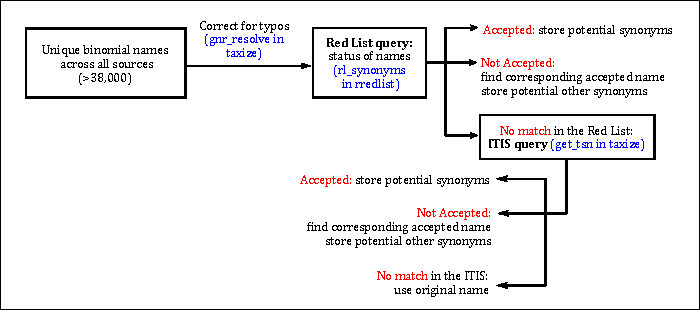
\includegraphics[scale=1.4]{figures/Chapter1/Taxonomic_corrections_chart}
\caption[Procedure used to identify the accepted names of species.]{\textbf{Procedure used to identify the accepted names of species.} I extracted, where possible, the accepted names of species from either the IUCN Red List or the Integrated Taxonomic Information System (ITIS).}
\label{chart_taxcor}
\end{figure}


%%%%%%%%%%%%%%%%%%%%%%%%%%%%%%%%%%%%%%%%%%%%%%%%%%%%%%%%%%%%%%%%%%%%%
%% table with references for trait data
\begin{table}[h!]
\renewcommand{\baselinestretch}{1}
\renewcommand{\arraystretch}{1.5}
\begin{center}\fontsize{9}{11}\selectfont
\caption[Data sources for each trait.]{\textbf{Data sources for each trait.} Abbreviations: A = amphibians; B = birds; BL = body length; BM = body mass; DA = diel activity time; GL = generation length; H = habitat data; LCS = litter or clutch size; L/ML = longevity or maximum longevity; M = mammals; MA = age at sexual maturity; R = reptiles; RS = range size; TL = trophic level. Note. Data sources may contain more traits than shown here. Tick marks in parentheses indicate that the trait was present in the data source but that another closely related trait with a better coverage was used instead. The tilde character ($\sim$) before a tick mark indicates that I derived trophic levels from species diet. $^1$ \url{http://datazone.birdlife.org/home}; $^2$ \url{https://www.iucnredlist.org/resources/spatial-data-download}; $^{3}$\url{http://apiv3.iucnredlist.org/api/v3/docs$\#$general}.} 
\label{datasources}
\begin{tabular}{|l|c|c|c|c|c|c|c|c|c|c|c|}
\hline
\multicolumn{1}{|c|}{\multirow{2}{*}{\textbf{Sources}}} & \multirow{2}{*}{\textbf{Taxa}} & \multicolumn{10}{c|}{\textbf{Traits}}                                                                                                       \\ \cline{3-12} 
\multicolumn{1}{|c|}{}                                  &                                & \textbf{BM} & \textbf{BL} & \textbf{L/ML} & \textbf{MA} & \textbf{GL} & \textbf{LCS} & \textbf{TL} & \textbf{DA} & \textbf{RS} & \textbf{H} \\ \hline
\citet{Oliveira2017}                                                & \multirow{4}{*}{Amphibians}    & (\checkmark )         & \checkmark            & (\checkmark )           & \checkmark            &             & \checkmark             & $\sim$\checkmark           & \checkmark            &             &            \\ \cline{1-1} \cline{3-12} 
\citet{Cooper2008}                                                  &                                &             &             &               &             &             & \checkmark             &             &             &             &            \\ \cline{1-1} \cline{3-12} \begin{comment}
\textit{Senior dataset}$^1$                                                  &                                &             & \checkmark            &               &             &             &              &             &             &             &            \\ \cline{1-1} \cline{3-12} \end{comment}
\citet{Sodhi2008}                                                   &                                &             & \checkmark            &               &             &             &              &             &             &             &            \\ \hline
\citet{Wilman2014}                                                  & \multirow{2}{*}{Birds}         & \checkmark            &             &               &             &             &              & $\sim$\checkmark           & \checkmark            &             &            \\ \cline{1-1} \cline{3-12} 
BirdLife$^1$                                                &                                & \checkmark            &             &               &             & \checkmark            &              &             &             &    \checkmark         &            \\ \hline
\citet{Jones2009}                                                   & \multirow{5}{*}{Mammals}       & \checkmark            & (\checkmark )         & (\checkmark )           & (\checkmark )         &             & \checkmark             &             & \checkmark            &             &            \\ \cline{1-1} \cline{3-12} 
\citet{Kissling2014}                                                &                                &             &             &               &             &             &              & \checkmark            &             &             &            \\ \cline{1-1} \cline{3-12} 
\citet{Gainsbury2018}                                               &                                &             &             &               &             &             &              & \checkmark            &             &             &            \\ \cline{1-1} \cline{3-12} 
\citet{Wilman2014}                                                   &                                & \checkmark            &             &               &             &             &              &             & \checkmark            &             &            \\ \cline{1-1} \cline{3-12} 
\citet{Pacifici2015}                                                 &                                & \checkmark            &             &          &        & \checkmark            &              &             &             &             &            \\ \hline
\citet{Scharf2015}                                                  & \multirow{10}{*}{Reptiles}      & \checkmark            &             & \checkmark              & (\checkmark )         &             & \checkmark             & \checkmark            & \checkmark            &             &            \\ \cline{1-1} \cline{3-12} 
\citet{Vidan2017}                                                   &                                &             &             &               &             &             &              &             & \checkmark            &             &            \\ \cline{1-1} \cline{3-12} 
\citet{Stark2018}                                                   &                                & \checkmark            &             & \checkmark              &             &             & \checkmark             &             & \checkmark            &             &            \\ \cline{1-1} \cline{3-12} 
\citet{Schwarz2017}                                                 &                                &             &             &               &             &             & \checkmark             &             &             &             &            \\ \cline{1-1} \cline{3-12} 
\citet{Novosolov2017}                                        &                                & \checkmark            &             &               &             &             &              & \checkmark            &             &             &            \\ \cline{1-1} \cline{3-12} 
\citet{Novosolov2013}                                         &                                &             &             &               &             &             & \checkmark             &             &             &             &            \\ \cline{1-1} \cline{3-12} 
\citet{Slavenko2016}                                            &                                & \checkmark            &             &               &             &             &              &             &             &             &            \\ \cline{1-1} \cline{3-12}
\citet{FeldmanGEB2016}                                            &                                & \checkmark            &             &               &             &             &              &             &             &             &            \\ \cline{1-1} \cline{3-12}
\citet{Meiri2018GEB}                                            &                                &            &             &               &       \checkmark       &             &       \checkmark        &     \checkmark         & \checkmark             &             &            \\ \cline{1-1} \cline{3-12}
\citet{Meiri2015}                                            &                                &             &             &               &             &             &              &       \checkmark                         &         \checkmark                       &      &            \\ \cline{1-1} \cline{3-12}
\citet{Roll2017}                                            &                                &             &             &               &             &             &              &                                &      & \checkmark       &           \\ \hline
\citet{Myhrvold2015}                                         & B, M, R      & \checkmark            & \checkmark            & \checkmark              & (\checkmark )         &             & \checkmark             &             &             &             &            \\\hline \cline{1-1} \cline{3-12} 
\citet{IUCN2020} $^{2}$                                           &            A, B, M                   &             &             &               &             &             &              &             &             & \checkmark             &  \\ \hline
\citet{IUCN2020} $^{3}$                                           &        All                         &             &             &               &             &             &              &             &             &             & \checkmark           \\ \hline

\end{tabular}
\end{center}
\end{table}

%%%%%%%%%%%%%%%%%%%%%%%%%%%%%%%%%%%%%%%%%%%%%%%%%%%%%%%%%%%%%%
%%%%%%%%%%%%%%%%%%%%%%%%%%%%%%%%%%%%%%%%%%%%%%%%%%%%%%%%%%%%%%




\subsubsection{Compilation methods}
For continuous traits, I took the median value within species when multiple estimates were available from different sources, after removal of any repeated values, which were assumed to represent estimates duplicated across secondary compilations and derived from the same underlying primary sources. Although intraspecific variation is increasingly being recognized to have important effects on ecological systems \citep{Bolnick2011, Siefert2015, DesRoches2018, GonzalezSuarez2012a}, it was not feasible to obtain measures of intraspecific variability from all sources; therefore, estimates were provided as a single measure for each species. For some species and some traits, measures were provided separately for females and males. In such cases, I first obtained the mean of these two measures.

Across sources, there were multiple traits related to each of body size and life span. For instance, body mass and/or body length information could be provided. Different proxies were also available for life span, such as the age at sexual maturity or generation length. In such cases, I focused on the trait presenting the highest coverage.

\begin{itemize}
\item \textbf{Body size}\\
Adult body mass estimates were compiled for mammals, birds and reptiles. Body length information was compiled for amphibians, because the coverage for body length was higher than that for body mass. Body mass and body length are known to scale allometrically, although the allometric relationship differs across amphibian clades \citep{Santini2018}. In the amphibian dataset, Pearson’s correlation coefficient between log(Body mass) and log(Body length) was 0.71 (data points shown in the Supporting Information, Appendix 2, S2.2, Figure \ref{SI2_amphibians}).
 
\item \textbf{Longevity}\\
I defined longevity as the life span of an individual and maximum longevity as the longest life span reported. I used closely related traits when longevity/maximum longevity was not available or when longevity/maximum longevity had a poorer coverage than a related trait. I selected the age at sexual maturity for amphibians; Pearson’s correlation coefficient between log(Age at sexual maturity) and log(Maximum longevity) was 0.55 (Supporting Information, Appendix 2, S2.2, Figure \ref{SI2_amphibians}). I compiled the generation length for mammals and birds. The correlation between log(Generation length) and log(Longevity) was 0.74 for mammals and 0.70 for birds (data points shown in the Supporting Information, Appendix 2, S2.2, Figure \ref{SI2_birdsmammals}). Finally, I used maximum longevity directly for reptiles.

\item \textbf{Litter or clutch size}\\
The number of offspring (litter size) or eggs (clutch size) was compiled directly from the sources and treated as equivalent across classes. I reported measures of central tendencies provided by the sources where applicable; otherwise, I calculated range midpoints (mean of smallest and largest reported litter/clutch sizes).

\item \textbf{Trophic level}\\
In all classes, species were described as omnivores, carnivores or herbivores. For reptiles and mammals, this information was compiled directly from the sources. For amphibians and birds, trophic levels were not provided. For these two classes, I inferred trophic levels from dietary information (Table \ref{datasources}). For birds, I used the primary diet (based on food items recorded as composing $\geq$50\% of the diet of a species). Diet for amphibians was described without respect to the percentage use of food items; simply as a binary record of whether or not food items were used. In both cases, species recorded to only consume plant-based resources (seeds, nectar, fruit or other plant material) were classified as herbivores. Species consuming only animal resources (invertebrates or vertebrates) were classified as carnivores. Species consuming a mixture of plant and animal resources were classified as omnivores.

\item \textbf{Activity time}\\
Species were described as being either nocturnal or non-nocturnal. Despite a higher resolution of activity time information in some of the sources (e.g., species being described as cathemeral, crepuscular or diurnal), I adopted the classification of the source with the lowest resolution (EltonTraits: \citet{Wilman2014}, for birds), in order to have consistent information across classes. As such, all species defined as diurnal, cathemeral or crepuscular were classified as non-nocturnal, as opposed to species classified as strictly nocturnal.

\item \textbf{Habitat breadth}\\
I used IUCN habitat data \citep{IUCN2020}, which describe species habitat preferences and the suitability and importance of each habitat. I defined habitat breadth as the number of habitats a species was known to use, using level 2 of the IUCN Habitat Classification Scheme for description of habitat types (divided into: Forest, Savanna, Shrubland, Grassland, Wetland, Rocky areas, Caves and subterranean, Desert, Marine, Marine intertidal or coastal/supratidal, Artificial, Introduced vegetation, and Other/Unknown.) Note that the total number of habitats, determined by including those that qualify as artificial, correlates positively with the number of natural habitats used (Figure \ref{Fig_HB_main}).

%% figure habitat breadth
\begin{figure}[h!]
\centering
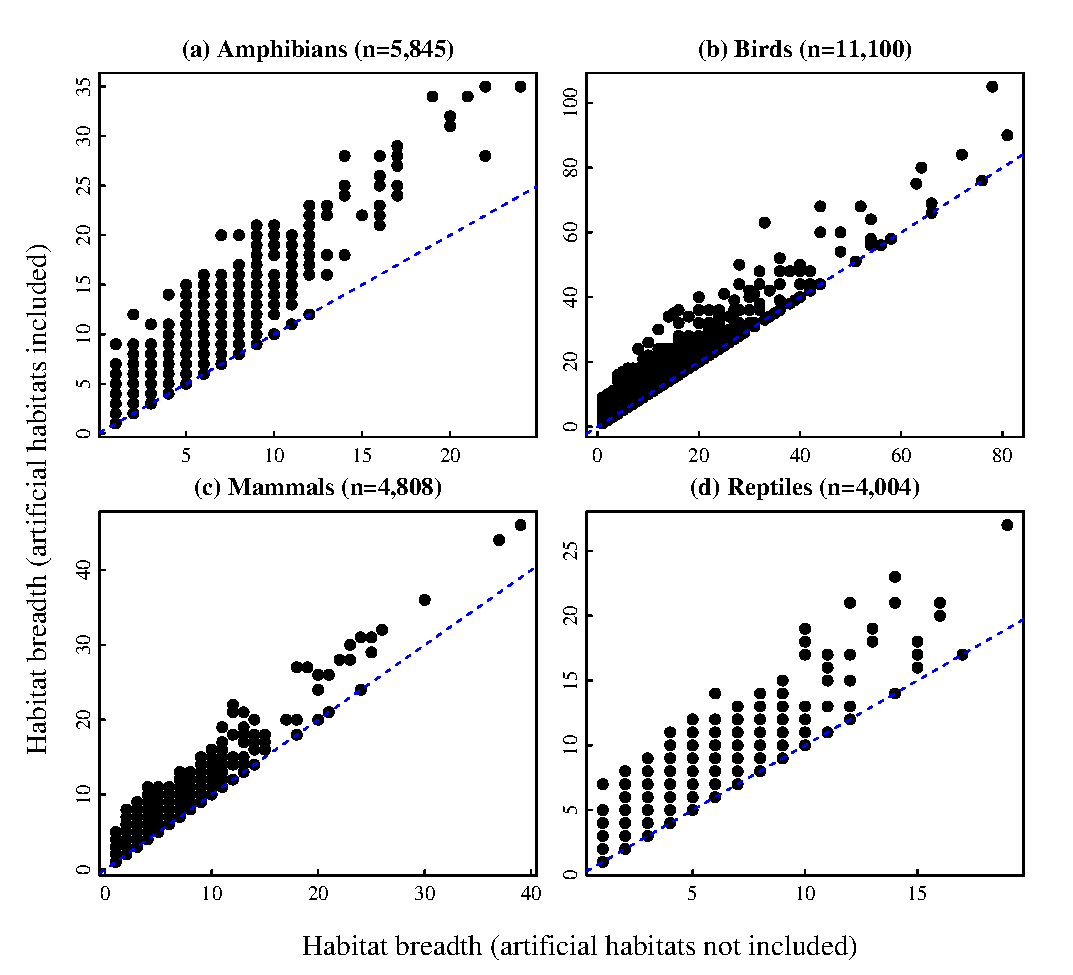
\includegraphics[scale=0.7]{figures/Chapter1/Fig_HB_main}
\caption[]{\textbf{Number of natural and artificial habitats used by a species against number of strictly natural habitats used by a species}. Pearson's correlation coefficients show a high positive correlation between these two metrics of habitat breadth in all terrestrial vertebrate classes: 0.92 for amphibians \textbf{(a)}, 0.95 for birds \textbf{(b)}, 0.94 for mammals \textbf{(c)}, and 0.90 for reptiles \textbf{(d)}.}
\label{Fig_HB_main}
\end{figure}


\item \textbf{Use of artificial habitats}\\
For a species, I recorded whether any artificial habitat was reported to be suitable in the IUCN habitat data.
\end{itemize}

Finally, the compiled datasets contain an additional column, `Note', where I reported species found to be extinct or extinct in the wild (EW). I used species Red List status and information from \citet{Meiri2018GEB} to flag such species. I reported 75 extinct/EW species for mammals, 160 for birds, 34 for amphibians and 53 for reptiles. It is likely that the datasets contain extinct species that I could not flag, because they were not recorded as extinct in the sources I used.

\newpage
\subsubsection{Phylogenies}
I used class-specific phylogenetic trees downloaded on 13 April 2020. For mammals, I used `complete' trees from \citet{Faurby2018, Faurby2020}, downloaded from \url{https://zenodo.org/record/3690867#.Xyc5wyhKhPZ}. For amphibians, birds and squamates, I obtained trees from \url{https://data.vertlife.org/}. The original sources were as follows: \citet{Jetz2012} for birds; \citet{Jetz2018} for amphibians; and \citet{Tonini2016} for squamates. For each class, a distribution of 1,000 trees was available. For plotting purposes, I obtained consensus trees using the TreeAnnotator program of the BEAST software \citep{Bouckaert2019}.

\subsubsection{Species distributions}
I obtained extent-of-occurrence distribution maps for reptiles from \citet{Roll2017}, available at: \url{https://datadryad.org/stash/dataset/doi:10.5061/dryad.83s7k} (downloaded 13 April 2020). For mammals and amphibians, species distribution maps were obtained from the IUCN Red List (\citet{IUCN2020}, downloaded 13 April 2020); for birds, they were obtained from BirdLife International (\url{http://datazone.birdlife.org/species/requestdis}, downloaded 17 April 2020).

For amphibians, mammals and birds, I selected areas of extant or probably extant presence only. Additionally, I selected areas where species were resident or present during the breeding season, and I excluded areas occupied during the non-breeding season or where species were considered vagrant.

In addition, for all classes, I excluded occupied areas that fell outside the known elevational limits of species, where such data were available. Lower and upper elevational limits were retrieved from the IUCN Red List (queried using the rredlist package) and were available for approximately half of the species (Supporting Information, Appendix 2, S2.3, Figure \ref{SI2_elev_limits}). Decreases in range sizes were observed after cutting distribution maps by the known elevational limits (Supporting Information, Appendix 2, S2.3, Figure \ref{SI2_cutalt_ranges}).

\subsection{Investigating gaps and biases in trait data}

I used trait coverage and completeness to investigate taxonomic, phylogenetic and spatial biases in the trait data. Table \ref{Chap1_samplesizes} summarizes the sample sizes (number of species) in each of the following analyses. Note that species for which completeness was 0\% were included in all analyses (for more details, see Figure \ref{1_Coverage}). Also note that I did not filter out species identified as extinct or extinct in the wild, because they represented a small proportion of the datasets (0.48\% for amphibians, 1.4\% for both birds and mammals, and 0.50\% for reptiles) and also because I could not exclude such species systematically, because it is likely that I did not flag them all.

%%%%%%%%%%%%%%%%%%%%%%%%%%%%%%%%%%%%%%%%%%%%%%%%%%%%%%%%%%%%%%
%%%%%%%%%%%%%%%%%%%%%%%%%%%%%%%%%%%%%%%%%%%%%%%%%%%%%%%%%%%%%%
\vskip 0.5cm

%  Table 2 sample sizes
\begin{table}[!htbp] 
\renewcommand{\baselinestretch}{1}
\renewcommand{\arraystretch}{1.5}
\begin{center}\fontsize{9}{11}\selectfont
\caption[Number of species for each analysis.]{\textbf{Number of species for each analysis.} All species represented in the trait datasets were included in (1). All species from the class-specific phylogenetic trees or from the distribution maps that matched with species in the trait datasets were included in (2) and (3).}
\label{Chap1_samplesizes}
\begin{tabular}{@{\extracolsep{5pt}} cccc} 
\\[-1.8ex]\hline 
\hline \\[-1.8ex]  & \textbf{(1) Taxonomic biases} & \textbf{(2) Phylogenetic biases} & \textbf{(3) Spatial biases} \\ 
\hline \\[-1.8ex] Amphibians & $6,990$ & $6,170$ & $5,650$ \\ 
Birds & $11,634$ & $8,315$ & $10,802$ \\ 
Mammals & $5,381$ & $5,171$ & $5,046$ \\ 
Reptiles & $10,612$ & $9,404$ & $9,382$\\
\hline \\[-1.8ex] 
\end{tabular} 
\end{center} 
\end{table} 
%%%%%%%%%%%%%%%%%%%%%%%%%%%%%%%%%%%%%%%%%%%%%%%%%%%%%%%%%%%%%%
%%%%%%%%%%%%%%%%%%%%%%%%%%%%%%%%%%%%%%%%%%%%%%%%%%%%%%%%%%%%%%


\subsubsection{Taxonomic biases}
I tested whether completeness varied across taxonomic class using pairwise Wilcoxon rank sum tests. I tested for the extent and performance of the taxonomic corrections by looking at trait coverage when taxonomic corrections are applied and when no correction is applied (Supporting Information, Appendix 2, S2.4, Figure \ref{SI_2_deltaCov_taxcor}).

\subsubsection{Phylogenetic biases}
Initially, to assess whether more closely related species were more likely to be similar in trait completeness, I estimated the phylogenetic signal in completeness with Pagel’s $\lambda$ \citep{Pagel1999} in each class. I used a bootstrapping approach, calculating $\lambda$ for each of 50 trees randomly sampled in each class (using the phylosig function of the phytools R package; \cite{Revell2012}). I then estimated the mean and 95\% confidence intervals (95\% CIs) of $\lambda$. Sample sizes for computing $\lambda$ (number of species represented in both the phylogenies and trait datasets) are shown in Table \ref{Chap1_samplesizes}.

I then plotted within-family median completeness in phylogenetic trees built at the family level, using the consensus trees. Within-family median completeness was calculated using taxonomic information in the trait datasets (sample sizes shown in Table \ref{Chap1_samplesizes}).

\subsubsection{Spatial biases}

I first investigated whether wider-ranging species were more likely to be better sampled than narrow-ranging species. I tested for a relationship between species range size and trait completeness. I fitted a generalized linear model with a Poisson error distribution (directly using the number of sampled traits, `N\textsubscript{traits}', rather than the proportion (completeness)). Class was added as a predictor interacting with range size; thus the model was:
\begin{center}
N\textsubscript{traits} $\sim$ log(Range size) $\ast$ Class. 
\end{center}
Second, I mapped assemblage-level median completeness. Assemblages were characterized at the pixel level at 50 km$^2$ resolution. I determined pixel-level composition and richness by stacking species geographical distributions. I then calculated median completeness across species in each pixel. I show the resulting maps for herptiles in the main text, and for mammals and birds in Supporting Information (Appendix 2, S2.5, Figure \ref{SI2_mediancomp_spatial}; median completeness was very high across most pixels for mammals and birds). In addition, I provide maps of assemblage-level mean completeness and standard deviation for all classes in the Supporting Information (Appendix 2, S2.5: Figures \ref{SI2_meancomp_spatial} and \ref{SI2_sdcomp_spatial} show corresponding maps; Figure \ref{SI2_sdcomp_sr} shows standard deviation against species richness).

I then tested for a spatial correlation between species richness and median completeness. Given that median completeness was very high across most pixels for mammals and birds, I fitted such models for herptiles only. I fitted spatial autoregressive lag models to explain assemblage-level median completeness as a function of species richness (using the function lagsarlm of the spatialreg package \citep{spatialreg1, spatialreg2, spatialreg3}). Given that responses could vary geographically, I included the biogeographical realm as an interacting factor (using the World Wide Fund for Nature (WWF) ecoregion shapefile to characterise realms, obtained from \url{https://www.worldwildlife.org/publications/terrestrial-ecoregions-of-the-world}); the considered realms were Afrotropics, Australasia, Indo-Malayan, Nearctic, Neotropics and Palaearctic. To improve normality, I arc-sin square-root transformed completeness values and log-transformed species richness. The lagsarlm function allows for a consideration of spatial autocorrelation in the dependent variable by estimating the autoregressive lag coefficient, $\rho$, associated with an n-by-n matrix of spatial weights, \textit{W}. The final model was:
\begin{center}
$\arcsin(\sqrt{\text{Completeness}})\sim \log(\text{Species richness}) \ast \text{realm} + \rho \cdot W \cdot \arcsin(\sqrt{\text{Completeness}})$.\\
\end{center}

The value of \textit{W} was estimated using the functions tri2nb and nb2listw of the spdep package \citep{spatialreg3, spdep1}. Fitting the model using all grid cells was computationally intractable; therefore, I randomly sampled cells for this analysis (using 30\% of the grid cells in each realm). I selected grid cells where species richness was higher than three to avoid sampling issues. I fitted separate models for amphibians and reptiles, because when adding class as an interacting predictor, the same cells (with the same coordinates) might be sampled for multiple classes, whereas the tri2nb function does not tolerate duplicated coordinates.

\section{Results}

\subsection{Taxonomic biases in trait information}
Trait coverage for mammals and birds was overall high (Figure \ref{1_Coverage}(a); mean and median coverage across traits: 89\% and 95\% for mammals; 84\% and 85\% for birds). In both cases, litter/clutch size was the trait with the poorest coverage (61\% for mammals and 59\% for birds). Coverage exceeded 80\% for all other traits (except  trophic level for birds, at 75\% coverage).

Conversely, trait coverage was more variable for herptiles, and poorer overall (Figure \ref{1_Coverage}(a); mean and median trait coverage: 47\% and 32\% for amphibians, 46\% and 38\% for reptiles). Coverage exceeded 80\% only for body size in both reptiles and amphibians and for habitat related traits in amphibians only. In all other cases coverage was  $<$55\%, with very little information available for longevity--related traits. 

Trait completeness (proportion of non-missing trait values for a species) reflected similar biases (Figure \ref{1_Coverage}(b)). The distribution of trait completeness varied significantly among classes (pairwise Wilcoxon rank sum test: p--value$<$0.0001 in all cases). Distributions were highly left skewed in mammals and birds (skewness: -2 and -1.6). 84\% of all mammalian species and 80\% of avian species fell in the 80--100\% completeness range. Moreover, the completeness distribution was moderately right skewed for reptiles (skewness: 0.4), and slightly right skewed for amphibians (skewness: 0.02). 56\% of all reptiles and 57\% of amphibians fell in the 0-50\% completeness range. 

\begin{figure}[h!]
\centering
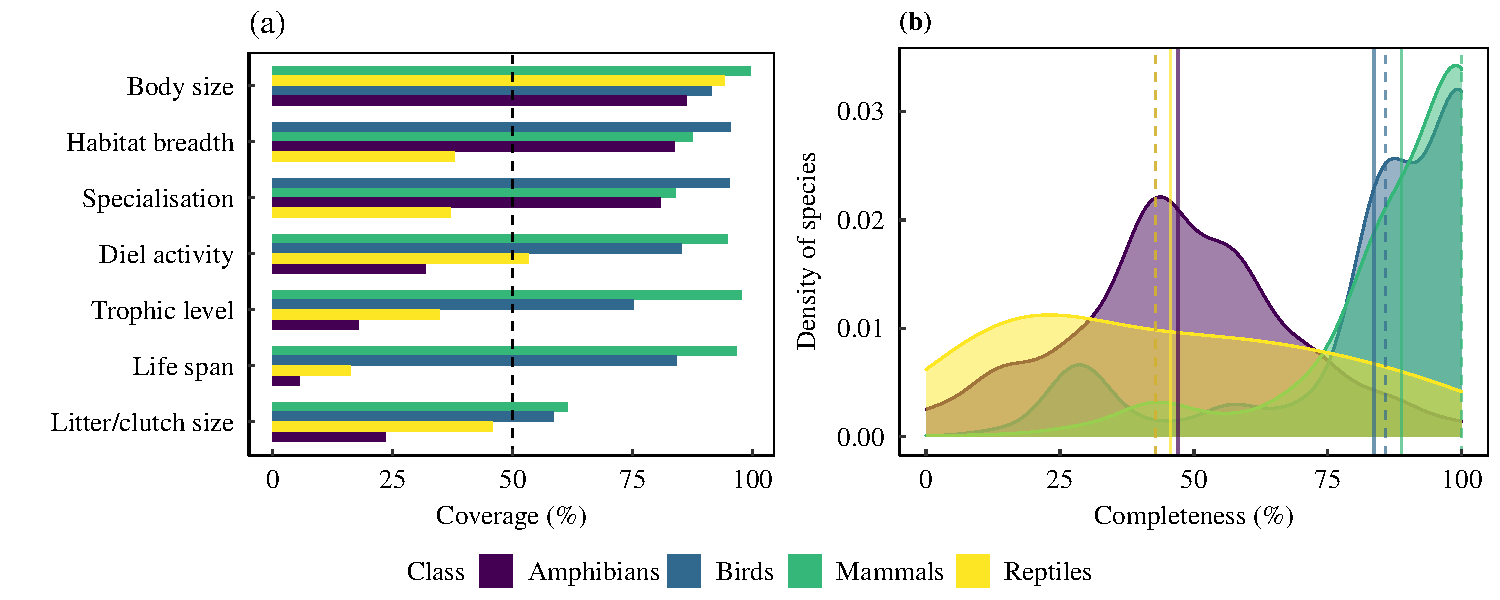
\includegraphics[scale=0.7]{figures/Chapter1/Figure1_revised}
\caption[Trait coverage and completeness across species.]{\textbf{Trait coverage and completeness across species.} \textbf{(a)} I defined coverage as the proportion of species for which an estimate is available for a given trait. The dashed line represents 50\% coverage. \textbf{(b)} Trait completeness is the proportion of estimated traits for a species. Here, I show the distribution of completeness. Continuous lines represent the mean trait completeness for each class, whereas dashed lines represent the median trait completeness. Note that there were species with 0\% completeness (230 species for amphibians -- 3.3\% of amphibian species in the trait dataset; 9 for birds -- 0.077\% of species; 7 for mammals -- 0.13\% of species; and 161 for reptiles -- 1.5\% of species). Species with 0\% completeness were retained in the datasets when there was information for traits I did not select in the analyses, but no known value for the traits I did select. For instance, the body mass of the amphibian species \textit{Rhinella centralis} was known, but other trait values (including body length) were missing, meaning that \textit{Rhinella centralis} had 0\% completeness for the set of traits I considered.}
\label{1_Coverage}
\end{figure}


\subsection{Phylogenetic biases in trait completeness}
As expected from the distribution of trait completeness in mammals and birds (Figure \ref{1_Coverage}), within-family median trait completeness was high across most tips of the phylogenetic trees (Supporting Information, Appendix 2, Figures \ref{SI2_phymammals} and \ref{SI2_phybirds}; I present the avian and mammalian phylogenies in the Supporting Information because there was little variation in completeness across tips). For birds, $\lambda$ was 0.71 ($\pm$ 0.0053). For mammals, $\lambda$ was 0.78 ($\pm$ 0.0035). This indicated that, despite completeness generally being high across tips, the sampling was not evenly distributed across the phylogeny.

In herptiles, clusters of families with similar median trait completeness appeared (Figure \ref{1_Phylo}). In amphibians, groups of families belonging to the order Anura (frogs) showed both the best and worst median completeness (Figure \ref{1_Phylo}(a)). The best-sampled families included the tailed frogs of the family Ascaphidae (two species) and species of the family Leiopelmatidae (four species endemic to New Zealand). The family Ceratobatrachidae (containing \textit{c.} 90 species occurring in Southeast Asia and in some Pacific islands), the family Ranidae (true frogs, 450 species considered here) and the family Rhacophoridae (shrub frogs, 382 species considered here) figured among the worst-sampled families. For amphibians, $\lambda$ was 0.63 ($\pm$ 0.0039). In reptiles, most snakes were poorly sampled, whereas families in other suborders appeared to be sampled better overall (Figure \ref{1_Phylo}(b)). Within snakes, the pythons, boas, the three species of the family Acrochordidae and the python-like species of the family Loxocemidae were better sampled than other snake families. In reptiles, $\lambda$ was 0.69 ($\pm$ 0.0032). The sampling in herptiles was thus also uneven with regard to the phylogeny.

It is important to underline that Figure \ref{1_Phylo} shows within-family median completeness, masking the considerable variation in species richness across families, hence masking potential important variation in completeness across species within families. For example, in the amphibian family Allophrynidae (three recognized species), the within-family median completeness was 50\%; but the dataset comprised two species of completeness 14\% and 86\%, respectively. I present similar plots to those in Figure \ref{1_Phylo} showing the within-family standard deviation in completeness in the Supporting Information (Appendix 2, Figure \ref{SI2_sd_phylo_herptiles}). Within-family standard deviation tended to increase with within-family species richness (Supporting Information, Appendix 2, Figure \ref{SI2_sd_sr_herptiles}).

\clearpage

\begin{figure}[h!]
\centering
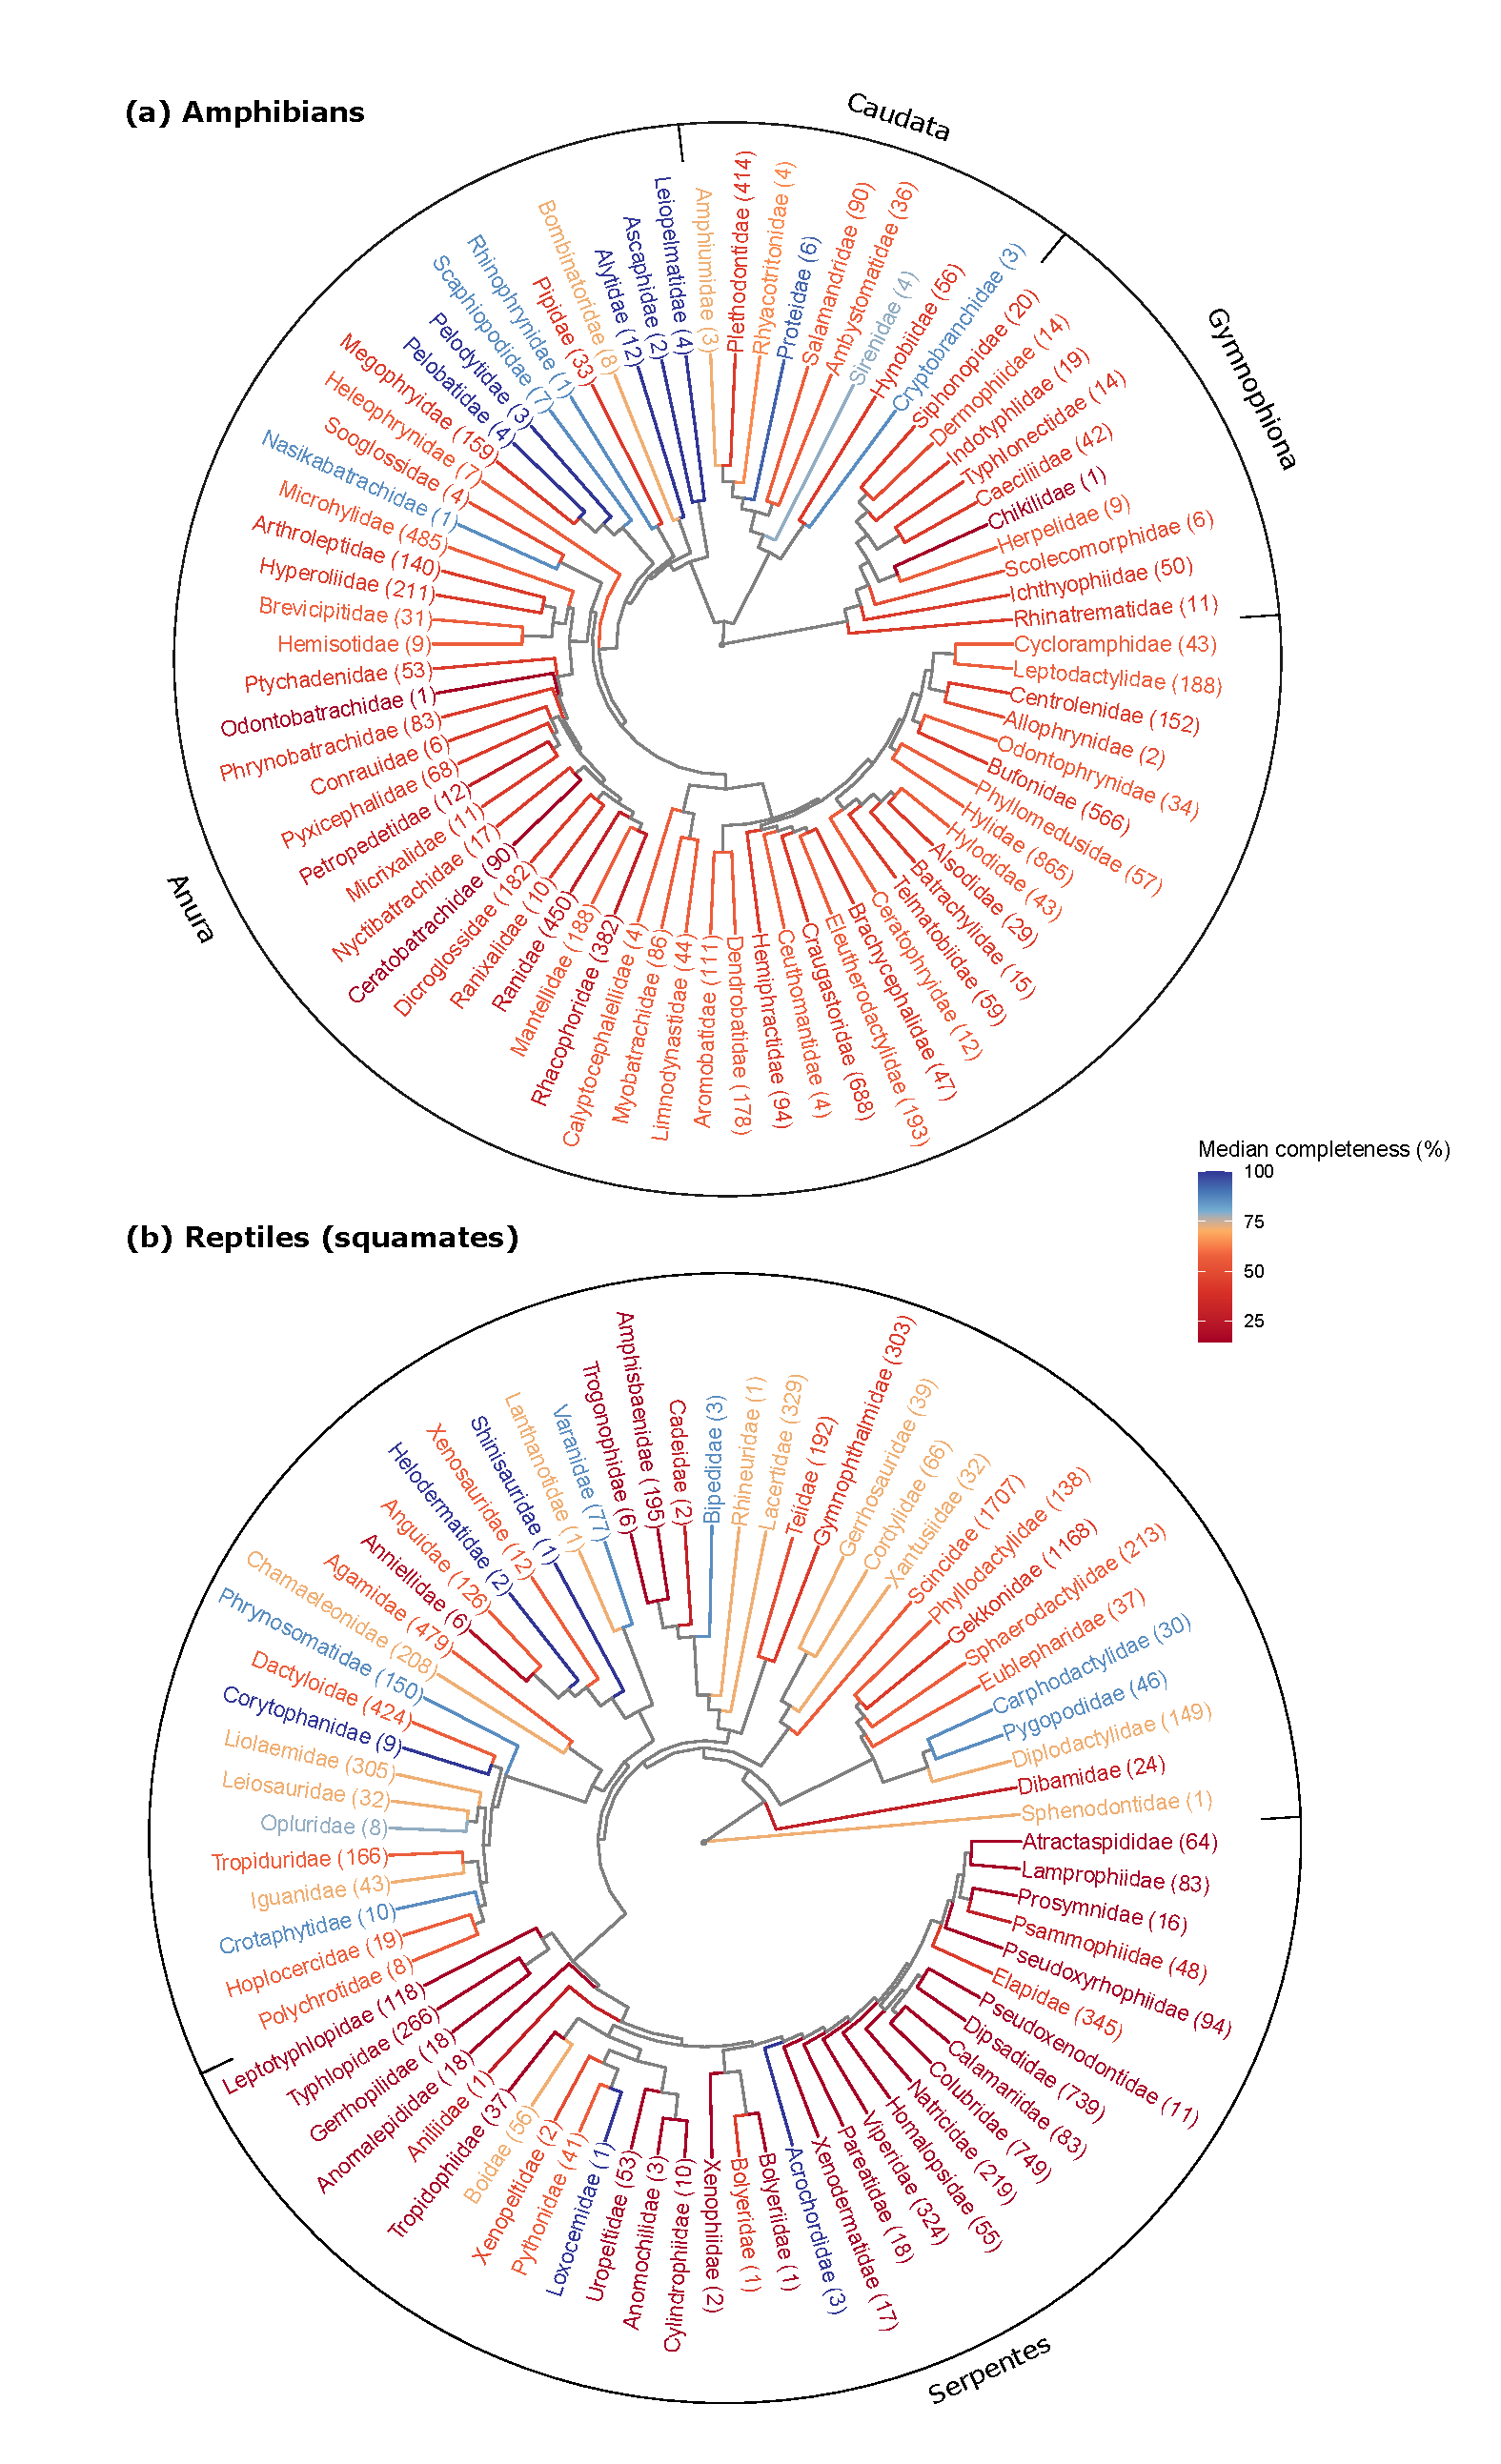
\includegraphics[scale=0.5]{figures/Chapter1/Figure_3}
\caption[Within-family median trait completeness in herptiles.]{\textbf{Within-family median trait completeness in herptiles.} The number next to each family name represents the number of species included in the calculation of the median.}
\label{1_Phylo}
\end{figure}

\clearpage

%% pick up the referencing to the SI figures here

\subsection{Spatial biases in trait completeness}
Range size was significantly correlated with the number of sampled traits. Larger range sizes were associated with a higher number of sampled traits (i.e., with higher completeness; Figure \ref{1_Range_size}; Supporting Information, Appendix 2, Table \ref{}). Similar results were obtained when using distribution maps not cut by elevational limits (Supporting Information, Appendix 2, Table \ref{}; Figure \ref{}). The rate of increase was steepest for reptiles, then for amphibians, then for birds and mammals (slope estimates for birds and mammals were not significantly different from each other; Supporting Information Table S1).

\begin{figure}[h!]
\centering
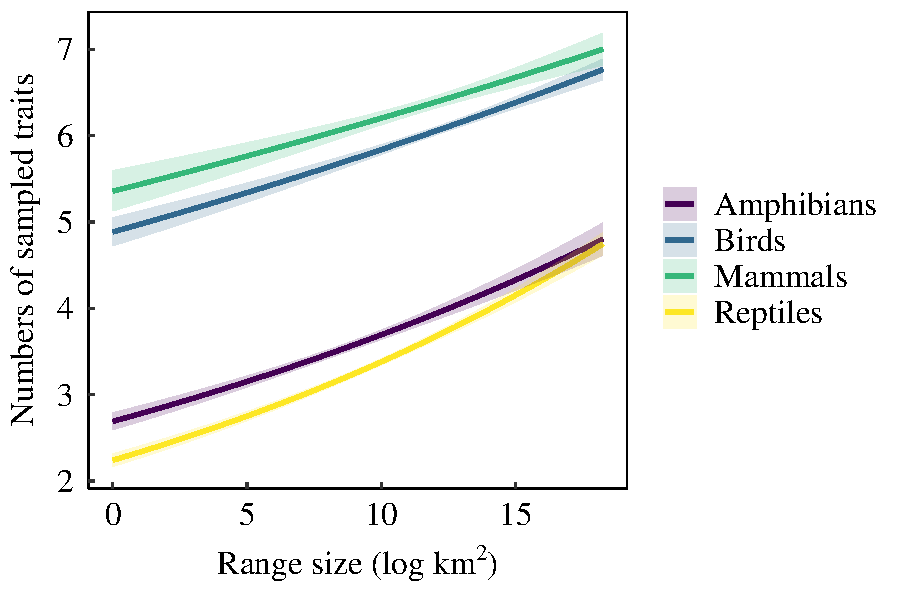
\includegraphics[scale=0.7]{figures/Chapter1/Figure_4}
\caption[Relationship between number of sampled traits and geographical range size]{\textbf{Relationship between number of sampled traits and geographical range size.} Models were fitted using a Poisson error distribution. Class was added as a predictor interacting with range size. Rates of increase in number of sampled traits with range size were not significantly different for mammals and birds but differed for reptiles and amphibians, with the steepest rates of increase for reptiles.}
\label{1_Range_size}
\end{figure}

There were marked spatial variations in median trait completeness in herptiles (Figure \ref{1_Map}). North America and Europe were well sampled for both amphibians and reptiles. Moreover, Southeast Asia and the Congo basin were on average less well sampled. In other regions, contrasting patterns emerged between amphibians and reptiles. For instance, median completeness was poorer for amphibians than for reptiles in Australia, but opposite patterns were observed in South America. As in the phylogenetic analyses, assemblage-level median completeness could mask potential important variation in completeness within species of a given assemblage. Assemblage-level mean and standard deviation maps are shown in the Supporting Information (Figures S8 and S9). There was a trend for increasing standard deviation with increasing species richness, with a larger spread in standard deviation at lower species richness (Supporting Information Figure S10).

\begin{figure}[h!]
\centering
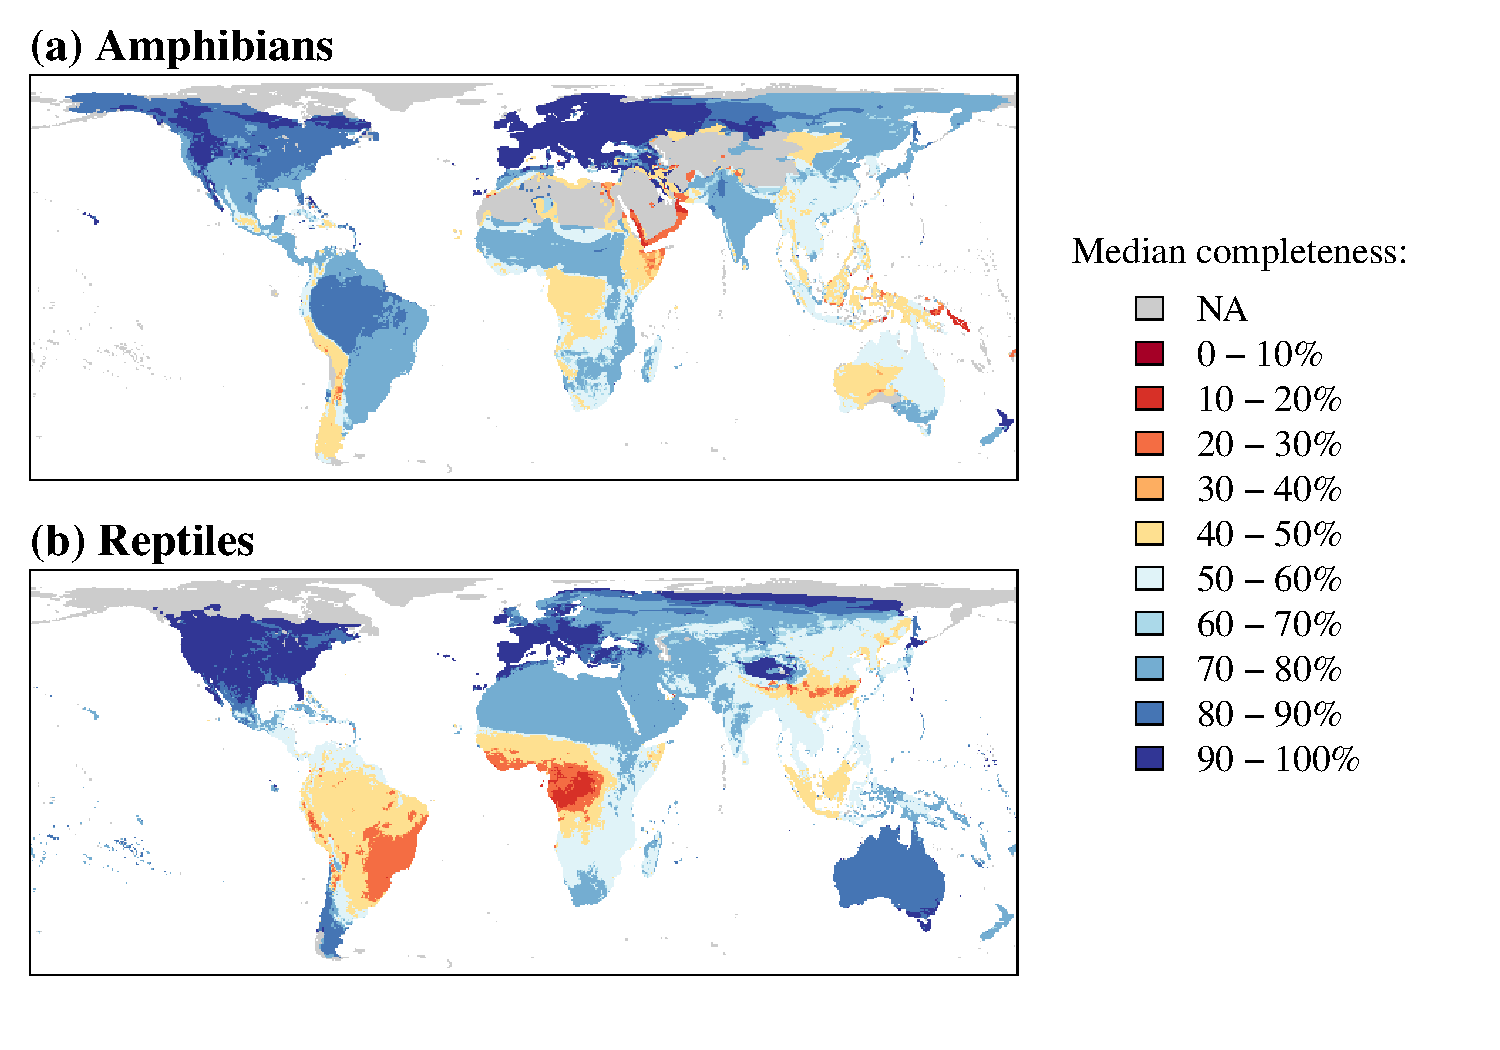
\includegraphics[scale=0.7]{figures/Chapter1/Figure_5}
\caption[Spatial distribution of assemblage-level median trait completeness in herptiles.]{\textbf{Spatial distribution of assemblage-level median trait completeness in herptiles.} Similar maps for birds and mammals are shown in the Supporting Information (Figure S7).}
\label{1_Map}
\end{figure}


Spatial models showed that species richness explained median trait completeness in herptiles in most realms (Figure 6; Supporting Information Tables S3 and S4); including spatial lags improved the models (reptiles: $\rho$ = 0.91, p-value < 0.0001; amphibians: $\rho$ = 0.92, p-value < 0.0001). For reptiles, completeness was negatively correlated with species richness in the most species-rich realms (Afrotropics, Indo-Malayan and Neotropics) and in the Palaearctic; the relationship was steepest in the Afrotropics and shallowest in the Palaearctic. In the Australasian and Nearctic realms, completeness tended to increase with species richness. For amphibians, negative relationships were observed in the Indo-Malay and Nearctic realms, whereas positive trends were observed in the Neotropics and the Palaearctic. The opposite trends between reptiles and amphibians observed in the Australasian and Neotropical realms reflected patterns observed on the maps. The Indo-Malayan was the only realm where median completeness tended to decrease with species richness for both reptiles and amphibians.

\clearpage
\begin{figure}[h!]
\centering
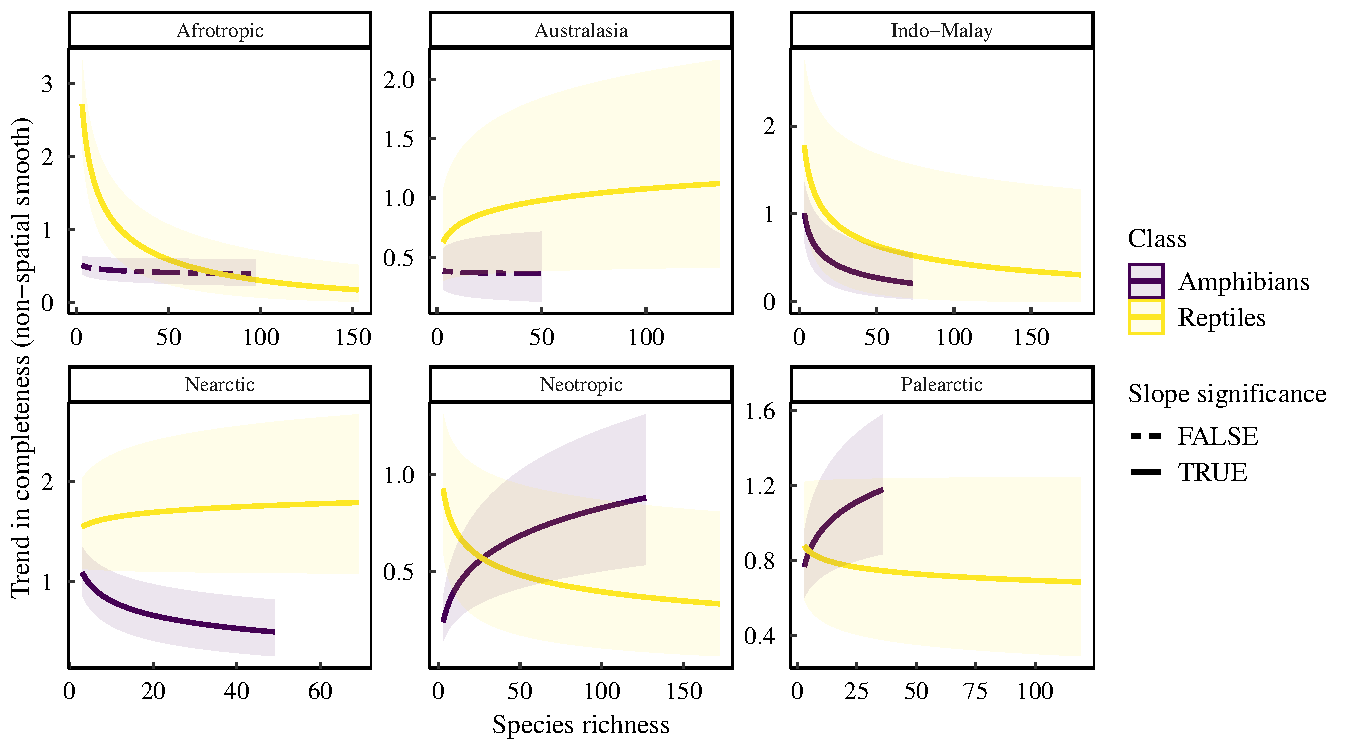
\includegraphics[scale=0.75]{figures/Chapter1/Figure_6}
\caption[Spatial model trends for herptiles.]{\textbf{Spatial model trends for herptiles.} The lines represent in-sample predictions ($\pm$ SE) for the trend components of the spatial models (trends after accounting for spatial autocorrelation).}
\label{1_Map}
\end{figure}


\section{Discussion}

The results of this chapter illustrate the taxonomic, spatial and phylogenetic dimensions of the knowledge gaps in trait data, termed the Raunkiæran shortfall by \citet{Hortal2015}. To the best of my knowledge, this work constitutes the first comparative assessment of global gaps for terrestrial vertebrate trait data, despite their use in numerous studies. I showed that the trait data present important taxonomic, spatial and phylogenetic biases, with contrasts in the availability of trait information between, on the one hand, herptiles and, on the other hand, birds and mammals.

Birds and mammals are globally well sampled for the set of traits I considered, even in the most species-rich assemblages. Moreover, the availability of trait information for herptiles is lower overall and phylogenetically and geographically biased. Several factors could interplay to shape these patterns. For instance, species that are more easily detectable (for example, wider ranging) and more charismatic are likely to be better sampled. Diverse socio-economic predictors could also contribute to geographical biases in trait data sampling; global biases in primary data collection are likely to be one of the most important contributors to the patterns I highlighted. Nevertheless, biases in the data could have been introduced at later stages, notably with the selection of sources and traits. The global compilation I obtained in this chapter reflects, in part, the interest and focus of the secondary data sources I used. It is possible that the addition of new sources from regional journals or other authorities could diminish spatial biases in the data by increasing coverage for certain areas. Nevertheless, I argue that by focusing on widely used traits, these results are likely to reflect the “true” availability of the data in primary sources and that the shortfalls for other, less used traits would be more pronounced.

I believe that the results presented here are robust to taxonomic uncertainty, although taxonomic matching might potentially be improved further using class-specific sources, such as the Reptile Database or AmphibiaWeb, for identification of synonyms (but see Supporting Information Appendix S9, Figure S16). I have made two versions of the data compilations available, one in which my own corrections were applied and one using the original binomial names of the sources, meaning that users are free to use their own taxonomic backbones and identify synonyms within the compilations.
I believe that taxonomic matching is a recurring issue when working across thousands of species. Taxonomic synonymy artefactually inflates the numbers of identified species, potentially lowering trait coverage (whereas clumping subspecies together can have the opposite effect). Tackling this problem is difficult \citep{Isaac2004, Jones2012}, notably because there is no global curated database recording the status of species names, and also because of the nature of taxonomy and the debates around the species concept \citep{May2011}. Nevertheless, taxonomic uncertainty can have important consequences. For instance, \citet{Cardoso2017} showed that inaccuracies and errors in species checklists contributed to the overestimation of plant diversity in the Amazon (but see \citet{Freeman2021}: the relative underdescription of species in tropical areas compared to temperate  areas (`taxonomic debt', also referred to as `latitudinal taxonomic gradient' by the authors) may lead to the underestimation of species richness at low latitudes).

Biases in trait data have important implications for conservation planning. Past studies have shown that narrow-ranged species, for which fewer trait data are available on average, have higher extinction risks \citep{Collen2016, Purvis2000, Ripple2017} and are more negatively impacted by anthropogenic pressures than wider-ranging species \citep{Newbold2018a}. Trait information is also less available for herptiles in tropical regions such as the Congo basin, Southeast Asia and South America, which are some of the most diverse areas of crucial importance for worldwide conservation \citep{Barlow2018}. Consequently, trait information is on average less available where potentially more crucial to conservation planning. Indeed, trait information can be incorporated into vulnerability assessments and, as such, can help to prioritize conservation efforts. Species traits have been found to mediate species responses to environmental changes across diverse taxonomic groups, and thus can inform on the sensitivity of species to anthropogenic pressures \citep{Flynn2009, Newbold2013, Nowakowski2017}. Traits are now commonly used to estimate species vulnerability or extinction risks \citep{Pacifici2015, RamirezBautista2020}. As opposed to trend-based approaches, which rely on historical population trends (changes in abundance or shifts in distributions) to predict species’ vulnerability and extinction risks, trait-based approaches rely on species’ intrinsic sensitivity to particular threats. The appeal of trait-based approaches to extinction risk estimation is that, by providing mechanistic insights, they diminish the amount of population information needed. If the responses of species to a threat consistently relate to certain traits, it is possible to generalize patterns across species for which population data are less available \citep{Verberk2013}. Integrating traits into vulnerability assessments is hence of particular interest when field monitoring of species population sizes or distributions is difficult to achieve, but biases in the data could mean that such information is lacking for some of the most vulnerable species.

%% 

Traits that influence species responses to environmental changes have been termed `response traits' (or `response-mediating traits'; \citet{Luck2012}), as opposed to `effect traits' that underpin ecosystem functioning \citep{Lavorel2002a}. For instance, relative brain size and longevity have been characterized as response traits in birds \citep{Newbold2013, Sayol2020}, whereas dietary characteristics (e.g., trophic levels or guilds) are both response and effect traits. \citet{Hortal2015} highlighted that, for plants, both response and effect traits have been investigated, whereas for vertebrates the research has been more focused on understanding species responses. This could be because the way vertebrate traits interact to shape some ecosystem processes has not yet been characterized well.

Ecosystem processes sustained by animals might be harder to quantify and might be influenced by a combination of traits. The traits compiled in this work are likely to have a role in diverse processes. Nevertheless, there was one important omission, in that I did not compile species diet in this chapter, potentially the most straightforward trait to link with diverse processes, such as grazing, pollination, scavenging and seed dispersal. From a practical perspective, I chose traits that had been estimated at least for some of the species in each class, and that were readily available. Diet was excluded because although estimates were available for amphibians, birds and mammals, there was no readily available database for reptilian diet. Movement or dispersal abilities were also excluded because information was not readily available for any class. Although I expect that species diet and dispersal abilities would present similar sampling biases to the ones presented in this work, the addition of such traits to the compilation would represent a valuable contribution and would notably facilitate studies looking at the functional roles of reptiles.

For practical reasons, I did not consider intraspecific trait variation. Intraspecific variation has been shown to have important effects on ecological systems, and a growing body of literature encourages trait-based research to include intraspecific variability \citep{Guralnick2016}. There have been several calls to produce open-access, global trait datasets \citep{Weiss2019}, including a representation of intraspecific trait variation \citep{Kissling2018}. Notably, \citet{Schneider2019} designed a framework to store and share inter- and intraspecific trait data, accompanied by an R package to standardize the data in a proposed format. Such a proposition could constitute an important step towards the unification of individual datasets into a single, comprehensive database for ecological trait data.

The current spatial and taxonomic gaps in trait data might limit our ability to scale studies up, whereas biases in the data can affect the validity of extrapolations to groups or areas that are undersampled. More generally, biases and gaps in biodiversity data can have important implications for ecological studies. Data gaps can hinder our ability to draw conclusions on observed macroecological patterns. For example, \citet{CHAUDHARY2016} proposed that marine species richness follows a bimodal distribution, peaking at mid-latitudinal locations, and argued that these patterns were not underpinned by knowledge gaps in species distributions. Nevertheless, \citet{Menegotto2018} attributed the tropical dip in marine species richness to a lack of species distribution data, explained by lower sampling efforts in tropical areas (`Wallacean' shortfall; \citet{Hortal2015}). Biases and gaps in trait data could also affect studies in closely related fields, such as functional ecology -- for instance, past studies have shown that functional diversity indices are sensitive to missing data \citep{Majekova2016, Pakeman2014} -- or community assembly \citep{Perronne2017}.

Ecologists should, therefore, take particular care when designing trait-based studies, because both data quality and data gaps are likely to influence the results and the generality of the conclusions. There exist diverse methods to deal with missing trait values, should data missingness be problematic. Complete removal of missing values (`case deletion') is commonly used but presents several issues, because it reduces sample size and statistical power and introduces potential bias in data subsamples \citep{Nakagawa2008}. For example, retaining complete cases only from the trait datasets would generate trait data disproportionally representative of mammals and birds, which would be problematic for conducting cross-taxon analysis on terrestrial vertebrates. As such, it is recommended that case deletion be applied only when data are missing completely at random, which is rarely the case \citep{Peugh2004}.

Alternatives to case deletion consist of filling in the gaps. In recent years, the development of imputation techniques has provided robust methods to handle missing data. Such imputation techniques have been used to complete trait datasets in recent studies \citep{Cooke2019b}. \citet{Penone2014} used a simulation approach to evaluate the performance of four of these techniques, namely PhyloPars \citep{Bruggeman2009}, random forest algorithms as implemented in R with missForest \citep{Stekhoven2016, Stekhoven2012}, multivariate imputation by chained equations (MICE; \citet{micepackage}) and k-nearest neighbour (kNN; \citet{Troyanskaya2001}). \citet{Penone2014} introduced missing values (10\%–80\%) in a complete trait dataset of carnivorans and measured imputation performance in different scenarios. Given that phylogenetic non-randomness in missing trait values can impact imputation accuracy, \citet{Penone2014} removed values in three different ways (completely at random; with a phylogenetic bias; and with a body mass bias). Out of the four techniques, missForest and PhyloPars performed best when species phylogenetic position was included as a predictor of missing trait values. Such imputations appeared to be robust even when trait coverage was as low as 40\%, which might be relevant for many reptilian and amphibian traits. The performance was not significantly affected by phylogenetic non-randomness of the data. Hence, missForest and PhyloPars appear to be well suited when traits are phylogenetically conserved, because they allow species phylogenetic position to be included as a predictor of missing trait values. The study by \citet{Penone2014} highlights that there are robust imputation techniques allowing to deal with incomplete trait data where biases might otherwise be problematic. Nevertheless, it is important to highlight that some imputation techniques, such as single or mean imputation, can be problematic because they do not allow an estimation of uncertainty and suffer from a lack of accuracy \citep{Nakagawa2008}; indeed, imputation techniques sometimes perform no better than case deletion. More work should be conducted to assess imputation performance in various contexts (see Johnson 2021), and the datasets compiled in this chapter might provide an opportunity for such studies.

%% Add Johnson ref for imputations??

Although robust imputation techniques can be useful for filling gaps in trait datasets, they are no substitute for continued data collection efforts. The results of this chapter show that data are particularly lacking in herptiles, notably in the Afrotropics, the Neotropics and the Indo-Malayan realms. For these areas, incorporating regional databases into existing datasets could contribute to the reduction of global gaps. I believe that both primary research and subsequent efforts to integrate new data and existing databases are required if we are to collectively strive towards the unification of trait databases.

To conclude, this work constitutes, to my knowledge, the first assessment of the global gaps and biases in terrestrial vertebrate trait information. I show that herptiles are undersampled compared with mammals and birds, with important spatial and phylogenetic variability in the availability of trait information. Imputation techniques are one possible solution to these problems. Nevertheless, I believe that primary research, combined with efforts to complete existing datasets, is the only way to fill the current data gaps genuinely and robustly. I hope that the compiled trait dataset and these findings can prove useful for guiding further data collection efforts and for conducting macroecological analyses.



\chapter{Intense human land uses negatively affect vertebrate functional diversity}
%% CHAPTER two -- global trait compilation

\section*{Keywords}
Terrestrial vertebrates; traits; coverage; completeness; taxonomic biases; spatial biases; phylogenetic biases.

\section*{Abstract}
Trait data are increasingly used in studies investigating the impacts of global changes on the structure and functioning of ecological communities. Despite a growing number of trait data collations for terrestrial vertebrates, there is to date no global assessment of the gaps and biases the data present. Here, I assess whether terrestrial vertebrate trait data are taxonomically, spatially and phylogenetically biased. I compile seven ecological traits and quantify coverage as the proportion of species for which an estimate is available. For a species, I define completeness as the proportion of non-missing values across traits. I assess whether coverage and completeness differ across classes and examine phylogenetic biases in trait data. To investigate spatial biases, I test whether wider-ranging species have more complete trait data than narrow-ranging species. Additionally, I test whether species-rich regions, which are of most concern for conservation, are less well-sampled than species-poor regions.
My results show that mammals and birds are well-sampled even in species-rich regions. For reptiles and amphibians (herptiles), only body size presents a high coverage (>80\%), as well as habitat related variables (for amphibians). Herptiles are poorly sampled for other traits. The shortfalls are particularly acute in some species-rich regions and for certain clades. Across all classes, geographically rarer species have less complete trait information. Hence, trait information is less available on average in some of the most diverse areas and in geographically rarer species, both critical for biodiversity conservation. Gaps in trait data may impede our ability to conduct large scale analyses, while biases can impact the validity of extrapolations. A short-term solution to the problem is to estimate missing trait data using imputation techniques, while a longer-term and more robust filling of existing gaps requires continued data collection efforts.

\section{Introduction}
Species traits are fundamental to ecological and evolutionary research. Comparative studies regularly use trait data across organisms to understand evolutionary processes and species coexistence \citep{Escudero2016, Zamudio2016}, to investigate global patterns of life forms and functions \citep{Diaz2016}, or to assess species’ vulnerability to environmental changes \citep{Bohm2016, Pacifici2015, Pearson2014}. Because traits influence species’ ability to cope with environmental changes \citep{Newbold2013} and underpin species’ contributions to ecosystem processes \citep{Lavorel2002a, Violle2007, Wong2018}, they play an increasingly important role in functional and conservation ecology.

Past and recent efforts to collate and release trait data in the public domain have facilitated the development of trait-based research. For instance, a global trait database has been published for plants \citep{Kattge2011}. As of May 2020, data from this database had been used in 297 publications since its release (Activity report, 18/06/2020, \url{https://www.try-db.org/TryWeb/Home.php}). Such databases hence constitute invaluable research tools and have the potential to greatly advance the field.

Vertebrates are one of the most studied taxa \citep{Titley2017}. There are now diverse sources of ecological traits for vertebrate groups (primates: \cite{Galan-Acedo2019}; mammals: `PanTHERIA', \cite{Jones2009}; amniotes: \cite{Myhrvold2015}; amphibians: ‘AmphiBIO’, \cite{Oliveira2017}). These datasets stem from important efforts to collate published estimates of trait data and make them readily available. Trait data have also been made available on online platforms (for instance, the Global Assessment of Reptile Distribution initiative: \url{http://www.gardinitiative.org/}; the IUCN Red List of Threatened Species: \url{https://www.iucnredlist.org/}; BirdLife data zone: \url{http://datazone.birdlife.org/home}).

Nevertheless, despite the importance of vertebrate species in global research outputs, there is no single source for vertebrate ecological traits. Consequently, researchers wishing to conduct comparative studies across vertebrate groups may have to collate trait data from a range of sources (such as in \citet{Cooke2019a, Cooke2019b} or in \citet{Gonzalez2018}), a time-consuming prerequisite which may be a limiting step of the research process. Indeed, collating data from heterogeneously-formatted sources presents many challenges \citep{Schneider2019}, particularly when working across a large number of species. For instance, traits may be measured differently across datasets; units may be inconsistent; and taxonomic resolution and nomenclature may vary.

The lack of a curated, readily available global database for vertebrate ecological traits impedes our ability to conduct cross-taxon comparative studies at global scales. However, efforts to collate data into a single database are limited by the availability of underlying data. Because there exist important gaps in biodiversity knowledge \citep{Hortal2015}, trait datasets are often incomplete, with many species lacking estimates for many traits. The incompleteness of ecological trait data at the species level has been termed the `Raunki{\ae}ran shortfall' by \citet{Hortal2015}. Furthermore, incomplete trait data are likely to be biased. Biases in trait data may be the consequence of uneven taxonomic and spatial collection effort, with a set of charismatic or easily detectable species being more completely sampled. For instance, \citet{Gonzalez-Suarez2012} investigated biases in global trait information in mammals. They notably found that the availability of mammalian trait data was geographically and phylogenetically biased, with larger and more widely distributed species being better sampled. In addition, data availability also differed across IUCN Red List extinction risk categories, with threatened species (Critically Endangered, Endangered or Vulnerable) being less well sampled for traits than non-threatened species (Least Concern or Near Threatened).

A major issue with incomplete, biased data is the introduction of bias in subsequent analyses. Assessing the amount of missing data as well as the so-called ‘missingness mechanism’-- whether missing data are missing at random, as opposed to there being systematic biases in the way missing values are distributed, see \citet{Baraldi2010} -- is an important prerequisite. Indeed, there exist diverse techniques to deal with data missingness. The simplest one consists of retaining complete cases only by filtering out missing values (case deletion, see \citet{Nakagawa2008}). Nevertheless, case deletion may lead to biased parameter estimates and erroneous conclusions when values are not missing at random \citep{Gonzalez-Suarez2012}. Therefore, it is critical to determine the most appropriate way to deal with data incompleteness. For instance, previous studies using terrestrial vertebrate trait data have employed multiple imputation techniques to fill in the gaps \citep{Gonzalez-Suarez2012, Cooke2019b}. Yet, imputation techniques could be sensitive to non-randomness in trait data. Phylogenetic biases (where some clades are under-sampled compared to other clades) could notably impact the performance of several imputation approaches. It is thus vital to characterise the gaps in trait data prior to any analysis. However, there has been no study to date investigating global patterns in the availability of trait data across terrestrial vertebrates.

Here, I aim to assess the global state of trait data in terrestrial vertebrates. I focus on a set of traits that are available across the four classes and that are commonly used by ecologists: body size; litter or clutch size; longevity; trophic level; activity time; habitat breath; and a measure of habitat specialisation. I quantify and compare the gaps in trait data across classes by calculating the coverage of each trait across species, and the completeness of trait estimates for each species (Box 1). I investigate taxonomic, spatial and phylogenetic biases in trait coverage and completeness.

Given that biodiversity research is globally biased towards birds and mammals \citep{Titley2017}, I hypothesise that herptiles are less well sampled for traits than mammals and birds, having both lower coverage and completeness.

Furthermore, building upon previous studies conducted on mammals \citep{Gonzalez-Suarez2012}, I hypothesize that species rarity influences completeness, focusing on species geographical range size as one aspect of rarity. Widely distributed species could be better sampled than narrowly distributed species because their ranges overlap with more study sites, regardless of their abundance. As such, I test whether species geographical range size explains trait completeness. 

It is well established that global research effort is distributed unequally \citep{ONU2015}, with patterns underpinned by various geographical and socioeconomic factors. For instance, countries with higher gross domestic product tend to host a larger number of research institutions \citep{Martin2012}. The proximity of research infrastructures and the accessibility of survey sites play an important part in explaining the global distribution of knowledge \citep{Hortal2015}. As a result of these factors, biodiversity data gaps tend to be greater in tropical areas \citep{Collen2008}. Tropical areas have the greatest species richness, and so these data biases are of great concern for biodiversity conservation. Whether species-rich regions are systematically under-sampled for traits compared to species-poor regions is thus important to assess, given the significance of species-rich areas for global conservation. Here, I investigate spatial biases in trait completeness, hypothesizing that species-rich areas are on average less well sampled than species-poor areas.

Finally, I investigate phylogenetic biases in the trait data. I assess whether particular clades have received more attention than others by looking for patterns in the distribution of trait completeness across the terminal branches of phylogenetic trees in each class.

\clearpage

\begin{mdframed}
\label{Trait_definition_box}
\textbf{Box 1. Definitions}\\
\textit{Trait:} Sensu stricto, a characteristic measurable at the level of an individual and that influences organismal fitness or performance \citep{Violle2007}. In this thesis, I broaden this definition to include `ecological' traits (e.g., the number of habitats used by a species), where the relationship of a species to the surrounding environment needs to be considered. Ecological traits may be estimated by aggregating data across multiple individuals.\\
\textit{Trait completeness:} For a given species, the proportion of traits for which an estimate is available.\\
\textit{Trait coverage:} For a given trait, the proportion of species for which an estimate is available.
\end{mdframed}


\section{Methods}

I produced class-specific trait datasets that were made available on figshare (DOI: \url{10.6084/m9.figshare.10075421}).
Data compilation and all analyses were conducted with R version 3.5.1 \citep{R_citation}.
Distribution maps were processed using both R and the ArcPy package available in ArcGIS v.10.6 \citep{ESRI} (implemented in Python 2.7; \citet{Python_citation}).

\subsection{Trait data collection}

\subsubsection{Sources and taxonomic matching}

I used freely accessible secondary sources in my compilation (Table \ref{datasources}), selected for their broad taxonomic coverage and/or for their frequent use in macroecological studies. Across sources, similar species could appear under synonymic names. This was a potential problem for matching sources by binomial names. Indeed, synonymy can artefactually decrease trait coverage, when trait information is not available across all synonyms. Notably, difficulties arise when species have been divided into several subspecies or when different subspecies are clumped together. Systematic manual checks could not be applied considering the scale of the data collection (there were $>$39,000 unique binomial names across sources). I developed a procedure aiming at identifying one accepted name for each of the binomial names found across sources. When I could not find an accepted name, I used the original name. Figure \ref{chart_taxcor} summarizes the main steps; similar solutions have been used in other large-scale studies \citep{Cooke2019b}.

Briefly, the procedure consisted of extracting synonyms from the IUCN \citep{IUCN2020} or from the Integrated Taxonomic Information System (ITIS; \url{https://www.itis.gov/}), using the rredlist \citep{rredlist} and taxize \citep{Chamberlain2013} R packages. One accepted name was assigned to each synonym. I produced a “Synonym” dataset that I have also made available. I then normalized taxonomy across sources by replacing binomial names with their identified accepted name where applicable.

Given that different taxonomic backbones could be used to correct for taxonomy, I make two versions of the trait compilations available (corrected and not corrected for taxonomy), meaning that users are free to apply their own corrections; for example, taxonomy could be aligned to that of class-specific sources, such as The Reptile Database, the American Museum of Natural History’s Amphibian Species of the World, the Mammal Diversity Database or the International Ornithological Congress World Bird List. Datasets corrected for taxonomy contain 11,634 species of birds, 5,381 mammals, 10,612 reptiles and 6,990 amphibians. Where no taxonomic correction was applied when matching sources, the compiled datasets contain 13,501 birds, 5,791 mammals, 11,012 reptiles and 8,583 amphibians. For more information, see the Supporting Information (Appendix 2, S2.1; Figure \ref{SI2_taxcor}).

%%%%%%%%%%%%%%%%%%%%%%%%%%%%%%%%%%%%%%%%%%%%%%%%%%%%%%%%%%%%%%%%%%%%%
%% figure 1: procedure for taxonomic checks
\vskip 1cm
\begin{figure}[h!]
\centering
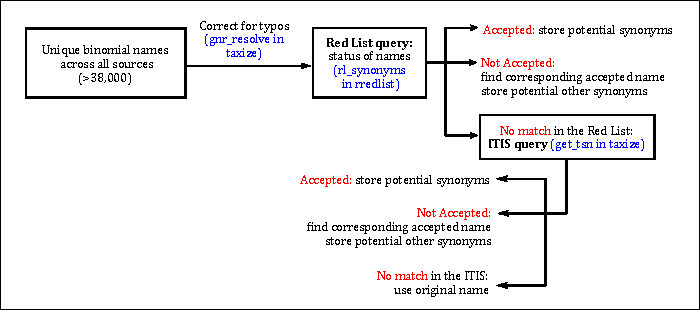
\includegraphics[scale=1.4]{figures/Chapter1/Taxonomic_corrections_chart}
\caption[Procedure used to identify the accepted names of species.]{\textbf{Procedure used to identify the accepted names of species.} I extracted, where possible, the accepted names of species from either the IUCN Red List or the Integrated Taxonomic Information System (ITIS).}
\label{chart_taxcor}
\end{figure}


%%%%%%%%%%%%%%%%%%%%%%%%%%%%%%%%%%%%%%%%%%%%%%%%%%%%%%%%%%%%%%%%%%%%%
%% table with references for trait data
\begin{table}[h!]
\renewcommand{\baselinestretch}{1}
\renewcommand{\arraystretch}{1.5}
\begin{center}\fontsize{9}{11}\selectfont
\caption[Data sources for each trait.]{\textbf{Data sources for each trait.} Abbreviations: A = amphibians; B = birds; BL = body length; BM = body mass; DA = diel activity time; GL = generation length; H = habitat data; LCS = litter or clutch size; L/ML = longevity or maximum longevity; M = mammals; MA = age at sexual maturity; R = reptiles; RS = range size; TL = trophic level. Note. Data sources may contain more traits than shown here. Tick marks in parentheses indicate that the trait was present in the data source but that another closely related trait with a better coverage was used instead. The tilde character ($\sim$) before a tick mark indicates that I derived trophic levels from species diet. $^1$ \url{http://datazone.birdlife.org/home}; $^2$ \url{https://www.iucnredlist.org/resources/spatial-data-download}; $^{3}$\url{http://apiv3.iucnredlist.org/api/v3/docs$\#$general}.} 
\label{datasources}
\begin{tabular}{|l|c|c|c|c|c|c|c|c|c|c|c|}
\hline
\multicolumn{1}{|c|}{\multirow{2}{*}{\textbf{Sources}}} & \multirow{2}{*}{\textbf{Taxa}} & \multicolumn{10}{c|}{\textbf{Traits}}                                                                                                       \\ \cline{3-12} 
\multicolumn{1}{|c|}{}                                  &                                & \textbf{BM} & \textbf{BL} & \textbf{L/ML} & \textbf{MA} & \textbf{GL} & \textbf{LCS} & \textbf{TL} & \textbf{DA} & \textbf{RS} & \textbf{H} \\ \hline
\citet{Oliveira2017}                                                & \multirow{4}{*}{Amphibians}    & (\checkmark )         & \checkmark            & (\checkmark )           & \checkmark            &             & \checkmark             & $\sim$\checkmark           & \checkmark            &             &            \\ \cline{1-1} \cline{3-12} 
\citet{Cooper2008}                                                  &                                &             &             &               &             &             & \checkmark             &             &             &             &            \\ \cline{1-1} \cline{3-12} \begin{comment}
\textit{Senior dataset}$^1$                                                  &                                &             & \checkmark            &               &             &             &              &             &             &             &            \\ \cline{1-1} \cline{3-12} \end{comment}
\citet{Sodhi2008}                                                   &                                &             & \checkmark            &               &             &             &              &             &             &             &            \\ \hline
\citet{Wilman2014}                                                  & \multirow{2}{*}{Birds}         & \checkmark            &             &               &             &             &              & $\sim$\checkmark           & \checkmark            &             &            \\ \cline{1-1} \cline{3-12} 
BirdLife$^1$                                                &                                & \checkmark            &             &               &             & \checkmark            &              &             &             &    \checkmark         &            \\ \hline
\citet{Jones2009}                                                   & \multirow{5}{*}{Mammals}       & \checkmark            & (\checkmark )         & (\checkmark )           & (\checkmark )         &             & \checkmark             &             & \checkmark            &             &            \\ \cline{1-1} \cline{3-12} 
\citet{Kissling2014}                                                &                                &             &             &               &             &             &              & \checkmark            &             &             &            \\ \cline{1-1} \cline{3-12} 
\citet{Gainsbury2018}                                               &                                &             &             &               &             &             &              & \checkmark            &             &             &            \\ \cline{1-1} \cline{3-12} 
\citet{Wilman2014}                                                   &                                & \checkmark            &             &               &             &             &              &             & \checkmark            &             &            \\ \cline{1-1} \cline{3-12} 
\citet{Pacifici2015}                                                 &                                & \checkmark            &             &          &        & \checkmark            &              &             &             &             &            \\ \hline
\citet{Scharf2015}                                                  & \multirow{10}{*}{Reptiles}      & \checkmark            &             & \checkmark              & (\checkmark )         &             & \checkmark             & \checkmark            & \checkmark            &             &            \\ \cline{1-1} \cline{3-12} 
\citet{Vidan2017}                                                   &                                &             &             &               &             &             &              &             & \checkmark            &             &            \\ \cline{1-1} \cline{3-12} 
\citet{Stark2018}                                                   &                                & \checkmark            &             & \checkmark              &             &             & \checkmark             &             & \checkmark            &             &            \\ \cline{1-1} \cline{3-12} 
\citet{Schwarz2017}                                                 &                                &             &             &               &             &             & \checkmark             &             &             &             &            \\ \cline{1-1} \cline{3-12} 
\citet{Novosolov2017}                                        &                                & \checkmark            &             &               &             &             &              & \checkmark            &             &             &            \\ \cline{1-1} \cline{3-12} 
\citet{Novosolov2013}                                         &                                &             &             &               &             &             & \checkmark             &             &             &             &            \\ \cline{1-1} \cline{3-12} 
\citet{Slavenko2016}                                            &                                & \checkmark            &             &               &             &             &              &             &             &             &            \\ \cline{1-1} \cline{3-12}
\citet{FeldmanGEB2016}                                            &                                & \checkmark            &             &               &             &             &              &             &             &             &            \\ \cline{1-1} \cline{3-12}
\citet{Meiri2018GEB}                                            &                                &            &             &               &       \checkmark       &             &       \checkmark        &     \checkmark         & \checkmark             &             &            \\ \cline{1-1} \cline{3-12}
\citet{Meiri2015}                                            &                                &             &             &               &             &             &              &       \checkmark                         &         \checkmark                       &      &            \\ \cline{1-1} \cline{3-12}
\citet{Roll2017}                                            &                                &             &             &               &             &             &              &                                &      & \checkmark       &           \\ \hline
\citet{Myhrvold2015}                                         & B, M, R      & \checkmark            & \checkmark            & \checkmark              & (\checkmark )         &             & \checkmark             &             &             &             &            \\\hline \cline{1-1} \cline{3-12} 
\citet{IUCN2020} $^{2}$                                           &            A, B, M                   &             &             &               &             &             &              &             &             & \checkmark             &  \\ \hline
\citet{IUCN2020} $^{3}$                                           &        All                         &             &             &               &             &             &              &             &             &             & \checkmark           \\ \hline

\end{tabular}
\end{center}
\end{table}

%%%%%%%%%%%%%%%%%%%%%%%%%%%%%%%%%%%%%%%%%%%%%%%%%%%%%%%%%%%%%%
%%%%%%%%%%%%%%%%%%%%%%%%%%%%%%%%%%%%%%%%%%%%%%%%%%%%%%%%%%%%%%




\subsubsection{Compilation methods}
For continuous traits, I took the median value within species when multiple estimates were available from different sources, after removal of any repeated values, which were assumed to represent estimates duplicated across secondary compilations and derived from the same underlying primary sources. Although intraspecific variation is increasingly being recognized to have important effects on ecological systems \citep{Bolnick2011, Siefert2015, DesRoches2018, GonzalezSuarez2012a}, it was not feasible to obtain measures of intraspecific variability from all sources; therefore, estimates were provided as a single measure for each species. For some species and some traits, measures were provided separately for females and males. In such cases, I first obtained the mean of these two measures.

Across sources, there were multiple traits related to each of body size and life span. For instance, body mass and/or body length information could be provided. Different proxies were also available for life span, such as the age at sexual maturity or generation length. In such cases, I focused on the trait presenting the highest coverage.

\begin{itemize}
\item \textbf{Body size}\\
Adult body mass estimates were compiled for mammals, birds and reptiles. Body length information was compiled for amphibians, because the coverage for body length was higher than that for body mass. Body mass and body length are known to scale allometrically, although the allometric relationship differs across amphibian clades \citep{Santini2018}. In the amphibian dataset, Pearson’s correlation coefficient between log(Body mass) and log(Body length) was 0.71 (data points shown in the Supporting Information, Appendix 2, S2.2, Figure \ref{SI2_amphibians}).
 
\item \textbf{Longevity}\\
I defined longevity as the life span of an individual and maximum longevity as the longest life span reported. I used closely related traits when longevity/maximum longevity was not available or when longevity/maximum longevity had a poorer coverage than a related trait. I selected the age at sexual maturity for amphibians; Pearson’s correlation coefficient between log(Age at sexual maturity) and log(Maximum longevity) was 0.55 (Supporting Information, Appendix 2, S2.2, Figure \ref{SI2_amphibians}). I compiled the generation length for mammals and birds. The correlation between log(Generation length) and log(Longevity) was 0.74 for mammals and 0.70 for birds (data points shown in the Supporting Information, Appendix 2, S2.2, Figure \ref{SI2_birdsmammals}). Finally, I used maximum longevity directly for reptiles.

\item \textbf{Litter or clutch size}\\
The number of offspring (litter size) or eggs (clutch size) was compiled directly from the sources and treated as equivalent across classes. I reported measures of central tendencies provided by the sources where applicable; otherwise, I calculated range midpoints (mean of smallest and largest reported litter/clutch sizes).

\item \textbf{Trophic level}\\
In all classes, species were described as omnivores, carnivores or herbivores. For reptiles and mammals, this information was compiled directly from the sources. For amphibians and birds, trophic levels were not provided. For these two classes, I inferred trophic levels from dietary information (Table \ref{datasources}). For birds, I used the primary diet (based on food items recorded as composing $\geq$50\% of the diet of a species). Diet for amphibians was described without respect to the percentage use of food items; simply as a binary record of whether or not food items were used. In both cases, species recorded to only consume plant-based resources (seeds, nectar, fruit or other plant material) were classified as herbivores. Species consuming only animal resources (invertebrates or vertebrates) were classified as carnivores. Species consuming a mixture of plant and animal resources were classified as omnivores.

\item \textbf{Activity time}\\
Species were described as being either nocturnal or non-nocturnal. Despite a higher resolution of activity time information in some of the sources (e.g., species being described as cathemeral, crepuscular or diurnal), I adopted the classification of the source with the lowest resolution (EltonTraits: \citet{Wilman2014}, for birds), in order to have consistent information across classes. As such, all species defined as diurnal, cathemeral or crepuscular were classified as non-nocturnal, as opposed to species classified as strictly nocturnal.

\item \textbf{Habitat breadth}\\
I used IUCN habitat data \citep{IUCN2020}, which describe species habitat preferences and the suitability and importance of each habitat. I defined habitat breadth as the number of habitats a species was known to use, using level 2 of the IUCN Habitat Classification Scheme for description of habitat types (divided into: Forest, Savanna, Shrubland, Grassland, Wetland, Rocky areas, Caves and subterranean, Desert, Marine, Marine intertidal or coastal/supratidal, Artificial, Introduced vegetation, and Other/Unknown.) Note that the total number of habitats, determined by including those that qualify as artificial, correlates positively with the number of natural habitats used (Figure \ref{Fig_HB_main}).

%% figure habitat breadth
\begin{figure}[h!]
\centering
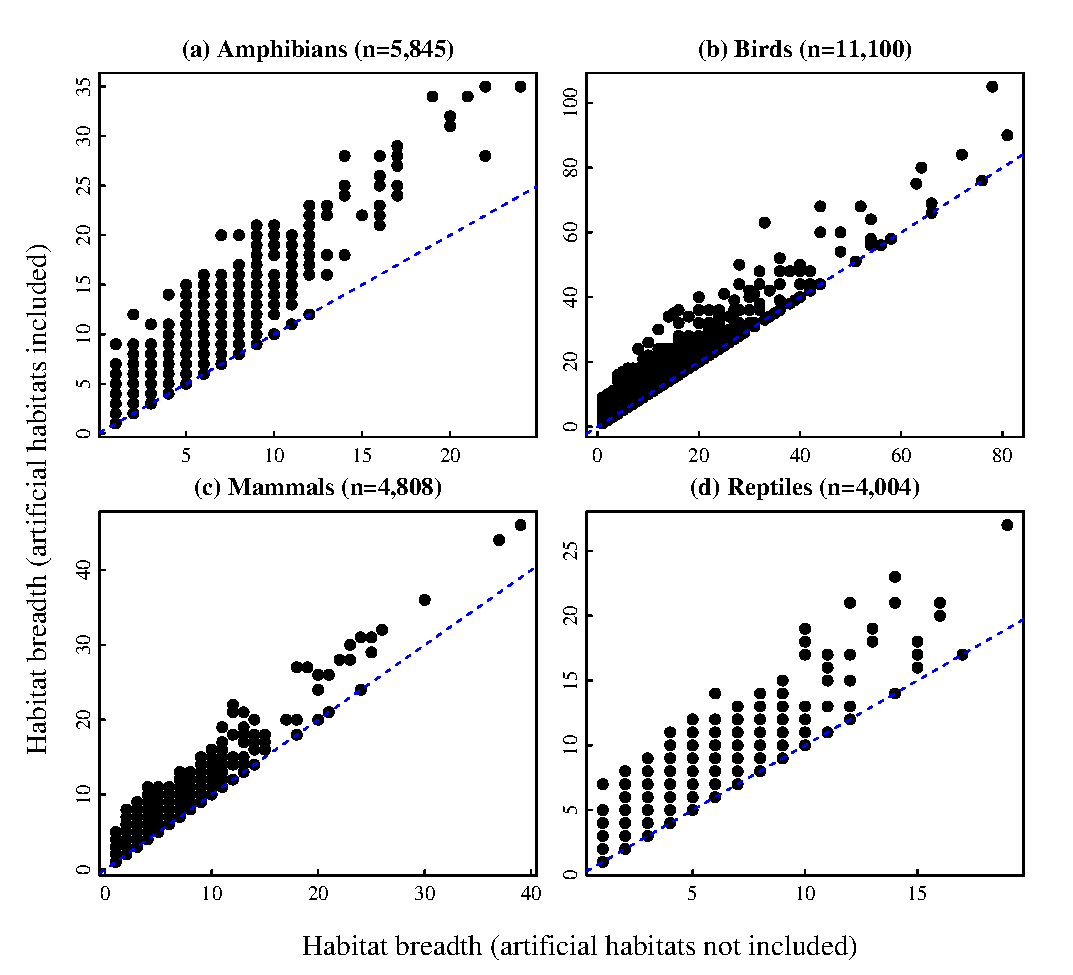
\includegraphics[scale=0.7]{figures/Chapter1/Fig_HB_main}
\caption[]{\textbf{Number of natural and artificial habitats used by a species against number of strictly natural habitats used by a species}. Pearson's correlation coefficients show a high positive correlation between these two metrics of habitat breadth in all terrestrial vertebrate classes: 0.92 for amphibians \textbf{(a)}, 0.95 for birds \textbf{(b)}, 0.94 for mammals \textbf{(c)}, and 0.90 for reptiles \textbf{(d)}.}
\label{Fig_HB_main}
\end{figure}


\item \textbf{Use of artificial habitats}\\
For a species, I recorded whether any artificial habitat was reported to be suitable in the IUCN habitat data.
\end{itemize}

Finally, the compiled datasets contain an additional column, `Note', where I reported species found to be extinct or extinct in the wild (EW). I used species Red List status and information from \citet{Meiri2018GEB} to flag such species. I reported 75 extinct/EW species for mammals, 160 for birds, 34 for amphibians and 53 for reptiles. It is likely that the datasets contain extinct species that I could not flag, because they were not recorded as extinct in the sources I used.

\newpage
\subsubsection{Phylogenies}
I used class-specific phylogenetic trees downloaded on 13 April 2020. For mammals, I used `complete' trees from \citet{Faurby2018, Faurby2020}, downloaded from \url{https://zenodo.org/record/3690867#.Xyc5wyhKhPZ}. For amphibians, birds and squamates, I obtained trees from \url{https://data.vertlife.org/}. The original sources were as follows: \citet{Jetz2012} for birds; \citet{Jetz2018} for amphibians; and \citet{Tonini2016} for squamates. For each class, a distribution of 1,000 trees was available. For plotting purposes, I obtained consensus trees using the TreeAnnotator program of the BEAST software \citep{Bouckaert2019}.

\subsubsection{Species distributions}
I obtained extent-of-occurrence distribution maps for reptiles from \citet{Roll2017}, available at: \url{https://datadryad.org/stash/dataset/doi:10.5061/dryad.83s7k} (downloaded 13 April 2020). For mammals and amphibians, species distribution maps were obtained from the IUCN Red List (\citet{IUCN2020}, downloaded 13 April 2020); for birds, they were obtained from BirdLife International (\url{http://datazone.birdlife.org/species/requestdis}, downloaded 17 April 2020).

For amphibians, mammals and birds, I selected areas of extant or probably extant presence only. Additionally, I selected areas where species were resident or present during the breeding season, and I excluded areas occupied during the non-breeding season or where species were considered vagrant.

In addition, for all classes, I excluded occupied areas that fell outside the known elevational limits of species, where such data were available. Lower and upper elevational limits were retrieved from the IUCN Red List (queried using the rredlist package) and were available for approximately half of the species (Supporting Information, Appendix 2, S2.3, Figure \ref{SI2_elev_limits}). Decreases in range sizes were observed after cutting distribution maps by the known elevational limits (Supporting Information, Appendix 2, S2.3, Figure \ref{SI2_cutalt_ranges}).

\subsection{Investigating gaps and biases in trait data}

I used trait coverage and completeness to investigate taxonomic, phylogenetic and spatial biases in the trait data. Table \ref{Chap1_samplesizes} summarizes the sample sizes (number of species) in each of the following analyses. Note that species for which completeness was 0\% were included in all analyses (for more details, see Figure \ref{1_Coverage}). Also note that I did not filter out species identified as extinct or extinct in the wild, because they represented a small proportion of the datasets (0.48\% for amphibians, 1.4\% for both birds and mammals, and 0.50\% for reptiles) and also because I could not exclude such species systematically, because it is likely that I did not flag them all.

%%%%%%%%%%%%%%%%%%%%%%%%%%%%%%%%%%%%%%%%%%%%%%%%%%%%%%%%%%%%%%
%%%%%%%%%%%%%%%%%%%%%%%%%%%%%%%%%%%%%%%%%%%%%%%%%%%%%%%%%%%%%%
\vskip 0.5cm

%  Table 2 sample sizes
\begin{table}[!htbp] 
\renewcommand{\baselinestretch}{1}
\renewcommand{\arraystretch}{1.5}
\begin{center}\fontsize{9}{11}\selectfont
\caption[Number of species for each analysis.]{\textbf{Number of species for each analysis.} All species represented in the trait datasets were included in (1). All species from the class-specific phylogenetic trees or from the distribution maps that matched with species in the trait datasets were included in (2) and (3).}
\label{Chap1_samplesizes}
\begin{tabular}{@{\extracolsep{5pt}} cccc} 
\\[-1.8ex]\hline 
\hline \\[-1.8ex]  & \textbf{(1) Taxonomic biases} & \textbf{(2) Phylogenetic biases} & \textbf{(3) Spatial biases} \\ 
\hline \\[-1.8ex] Amphibians & $6,990$ & $6,170$ & $5,650$ \\ 
Birds & $11,634$ & $8,315$ & $10,802$ \\ 
Mammals & $5,381$ & $5,171$ & $5,046$ \\ 
Reptiles & $10,612$ & $9,404$ & $9,382$\\
\hline \\[-1.8ex] 
\end{tabular} 
\end{center} 
\end{table} 
%%%%%%%%%%%%%%%%%%%%%%%%%%%%%%%%%%%%%%%%%%%%%%%%%%%%%%%%%%%%%%
%%%%%%%%%%%%%%%%%%%%%%%%%%%%%%%%%%%%%%%%%%%%%%%%%%%%%%%%%%%%%%


\subsubsection{Taxonomic biases}
I tested whether completeness varied across taxonomic class using pairwise Wilcoxon rank sum tests. I tested for the extent and performance of the taxonomic corrections by looking at trait coverage when taxonomic corrections are applied and when no correction is applied (Supporting Information, Appendix 2, S2.4, Figure \ref{SI_2_deltaCov_taxcor}).

\subsubsection{Phylogenetic biases}
Initially, to assess whether more closely related species were more likely to be similar in trait completeness, I estimated the phylogenetic signal in completeness with Pagel’s $\lambda$ \citep{Pagel1999} in each class. I used a bootstrapping approach, calculating $\lambda$ for each of 50 trees randomly sampled in each class (using the phylosig function of the phytools R package; \cite{Revell2012}). I then estimated the mean and 95\% confidence intervals (95\% CIs) of $\lambda$. Sample sizes for computing $\lambda$ (number of species represented in both the phylogenies and trait datasets) are shown in Table \ref{Chap1_samplesizes}.

I then plotted within-family median completeness in phylogenetic trees built at the family level, using the consensus trees. Within-family median completeness was calculated using taxonomic information in the trait datasets (sample sizes shown in Table \ref{Chap1_samplesizes}).

\subsubsection{Spatial biases}

I first investigated whether wider-ranging species were more likely to be better sampled than narrow-ranging species. I tested for a relationship between species range size and trait completeness. I fitted a generalized linear model with a Poisson error distribution (directly using the number of sampled traits, `N\textsubscript{traits}', rather than the proportion (completeness)). Class was added as a predictor interacting with range size; thus the model was:
\begin{center}
N\textsubscript{traits} $\sim$ log(Range size) $\ast$ Class. 
\end{center}
Second, I mapped assemblage-level median completeness. Assemblages were characterized at the pixel level at 50 km$^2$ resolution. I determined pixel-level composition and richness by stacking species geographical distributions. I then calculated median completeness across species in each pixel. I show the resulting maps for herptiles in the main text, and for mammals and birds in Supporting Information (Appendix 2, S2.5, Figure \ref{SI2_mediancomp_spatial}; median completeness was very high across most pixels for mammals and birds). In addition, I provide maps of assemblage-level mean completeness and standard deviation for all classes in the Supporting Information (Appendix 2, S2.5: Figures \ref{SI2_meancomp_spatial} and \ref{SI2_sdcomp_spatial} show corresponding maps; Figure \ref{SI2_sdcomp_sr} shows standard deviation against species richness).

I then tested for a spatial correlation between species richness and median completeness. Given that median completeness was very high across most pixels for mammals and birds, I fitted such models for herptiles only. I fitted spatial autoregressive lag models to explain assemblage-level median completeness as a function of species richness (using the function lagsarlm of the spatialreg package \citep{spatialreg1, spatialreg2, spatialreg3}). Given that responses could vary geographically, I included the biogeographical realm as an interacting factor (using the World Wide Fund for Nature (WWF) ecoregion shapefile to characterise realms, obtained from \url{https://www.worldwildlife.org/publications/terrestrial-ecoregions-of-the-world}); the considered realms were Afrotropics, Australasia, Indo-Malayan, Nearctic, Neotropics and Palaearctic. To improve normality, I arc-sin square-root transformed completeness values and log-transformed species richness. The lagsarlm function allows for a consideration of spatial autocorrelation in the dependent variable by estimating the autoregressive lag coefficient, $\rho$, associated with an n-by-n matrix of spatial weights, \textit{W}. The final model was:
\begin{center}
$\arcsin(\sqrt{\text{Completeness}})\sim \log(\text{Species richness}) \ast \text{realm} + \rho \cdot W \cdot \arcsin(\sqrt{\text{Completeness}})$.\\
\end{center}

The value of \textit{W} was estimated using the functions tri2nb and nb2listw of the spdep package \citep{spatialreg3, spdep1}. Fitting the model using all grid cells was computationally intractable; therefore, I randomly sampled cells for this analysis (using 30\% of the grid cells in each realm). I selected grid cells where species richness was higher than three to avoid sampling issues. I fitted separate models for amphibians and reptiles, because when adding class as an interacting predictor, the same cells (with the same coordinates) might be sampled for multiple classes, whereas the tri2nb function does not tolerate duplicated coordinates.

\section{Results}

\subsection{Taxonomic biases in trait information}
Trait coverage for mammals and birds was overall high (Figure \ref{1_Coverage}(a); mean and median coverage across traits: 89\% and 95\% for mammals; 84\% and 85\% for birds). In both cases, litter/clutch size was the trait with the poorest coverage (61\% for mammals and 59\% for birds). Coverage exceeded 80\% for all other traits (except  trophic level for birds, at 75\% coverage).

Conversely, trait coverage was more variable for herptiles, and poorer overall (Figure \ref{1_Coverage}(a); mean and median trait coverage: 47\% and 32\% for amphibians, 46\% and 38\% for reptiles). Coverage exceeded 80\% only for body size in both reptiles and amphibians and for habitat related traits in amphibians only. In all other cases coverage was  $<$55\%, with very little information available for longevity--related traits. 

Trait completeness (proportion of non-missing trait values for a species) reflected similar biases (Figure \ref{1_Coverage}(b)). The distribution of trait completeness varied significantly among classes (pairwise Wilcoxon rank sum test: p--value$<$0.0001 in all cases). Distributions were highly left skewed in mammals and birds (skewness: -2 and -1.6). 84\% of all mammalian species and 80\% of avian species fell in the 80--100\% completeness range. Moreover, the completeness distribution was moderately right skewed for reptiles (skewness: 0.4), and slightly right skewed for amphibians (skewness: 0.02). 56\% of all reptiles and 57\% of amphibians fell in the 0-50\% completeness range. 

\begin{figure}[h!]
\centering
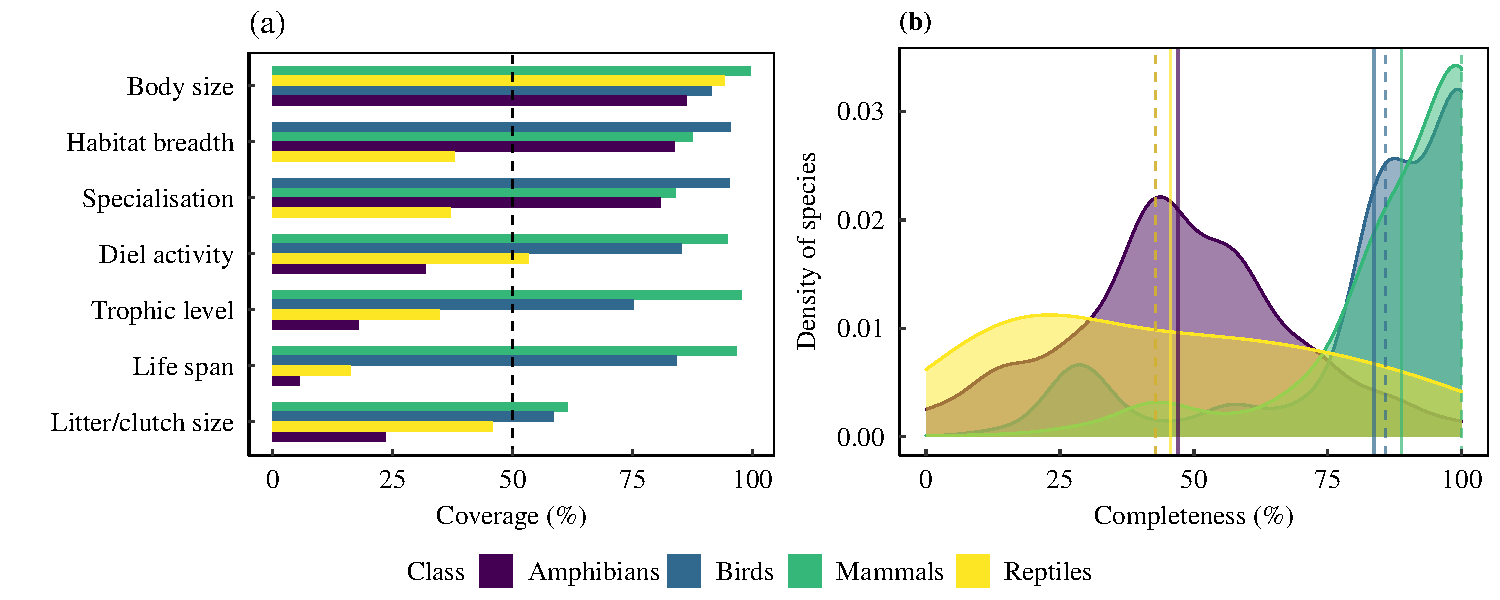
\includegraphics[scale=0.7]{figures/Chapter1/Figure1_revised}
\caption[Trait coverage and completeness across species.]{\textbf{Trait coverage and completeness across species.} \textbf{(a)} I defined coverage as the proportion of species for which an estimate is available for a given trait. The dashed line represents 50\% coverage. \textbf{(b)} Trait completeness is the proportion of estimated traits for a species. Here, I show the distribution of completeness. Continuous lines represent the mean trait completeness for each class, whereas dashed lines represent the median trait completeness. Note that there were species with 0\% completeness (230 species for amphibians -- 3.3\% of amphibian species in the trait dataset; 9 for birds -- 0.077\% of species; 7 for mammals -- 0.13\% of species; and 161 for reptiles -- 1.5\% of species). Species with 0\% completeness were retained in the datasets when there was information for traits I did not select in the analyses, but no known value for the traits I did select. For instance, the body mass of the amphibian species \textit{Rhinella centralis} was known, but other trait values (including body length) were missing, meaning that \textit{Rhinella centralis} had 0\% completeness for the set of traits I considered.}
\label{1_Coverage}
\end{figure}


\subsection{Phylogenetic biases in trait completeness}
As expected from the distribution of trait completeness in mammals and birds (Figure \ref{1_Coverage}), within-family median trait completeness was high across most tips of the phylogenetic trees (Supporting Information, Appendix 2, Figures \ref{SI2_phymammals} and \ref{SI2_phybirds}; I present the avian and mammalian phylogenies in the Supporting Information because there was little variation in completeness across tips). For birds, $\lambda$ was 0.71 ($\pm$ 0.0053). For mammals, $\lambda$ was 0.78 ($\pm$ 0.0035). This indicated that, despite completeness generally being high across tips, the sampling was not evenly distributed across the phylogeny.

In herptiles, clusters of families with similar median trait completeness appeared (Figure \ref{1_Phylo}). In amphibians, groups of families belonging to the order Anura (frogs) showed both the best and worst median completeness (Figure \ref{1_Phylo}(a)). The best-sampled families included the tailed frogs of the family Ascaphidae (two species) and species of the family Leiopelmatidae (four species endemic to New Zealand). The family Ceratobatrachidae (containing \textit{c.} 90 species occurring in Southeast Asia and in some Pacific islands), the family Ranidae (true frogs, 450 species considered here) and the family Rhacophoridae (shrub frogs, 382 species considered here) figured among the worst-sampled families. For amphibians, $\lambda$ was 0.63 ($\pm$ 0.0039). In reptiles, most snakes were poorly sampled, whereas families in other suborders appeared to be sampled better overall (Figure \ref{1_Phylo}(b)). Within snakes, the pythons, boas, the three species of the family Acrochordidae and the python-like species of the family Loxocemidae were better sampled than other snake families. In reptiles, $\lambda$ was 0.69 ($\pm$ 0.0032). The sampling in herptiles was thus also uneven with regard to the phylogeny.

It is important to underline that Figure \ref{1_Phylo} shows within-family median completeness, masking the considerable variation in species richness across families, hence masking potential important variation in completeness across species within families. For example, in the amphibian family Allophrynidae (three recognized species), the within-family median completeness was 50\%; but the dataset comprised two species of completeness 14\% and 86\%, respectively. I present similar plots to those in Figure \ref{1_Phylo} showing the within-family standard deviation in completeness in the Supporting Information (Appendix 2, Figure \ref{SI2_sd_phylo_herptiles}). Within-family standard deviation tended to increase with within-family species richness (Supporting Information, Appendix 2, Figure \ref{SI2_sd_sr_herptiles}).

\clearpage

\begin{figure}[h!]
\centering
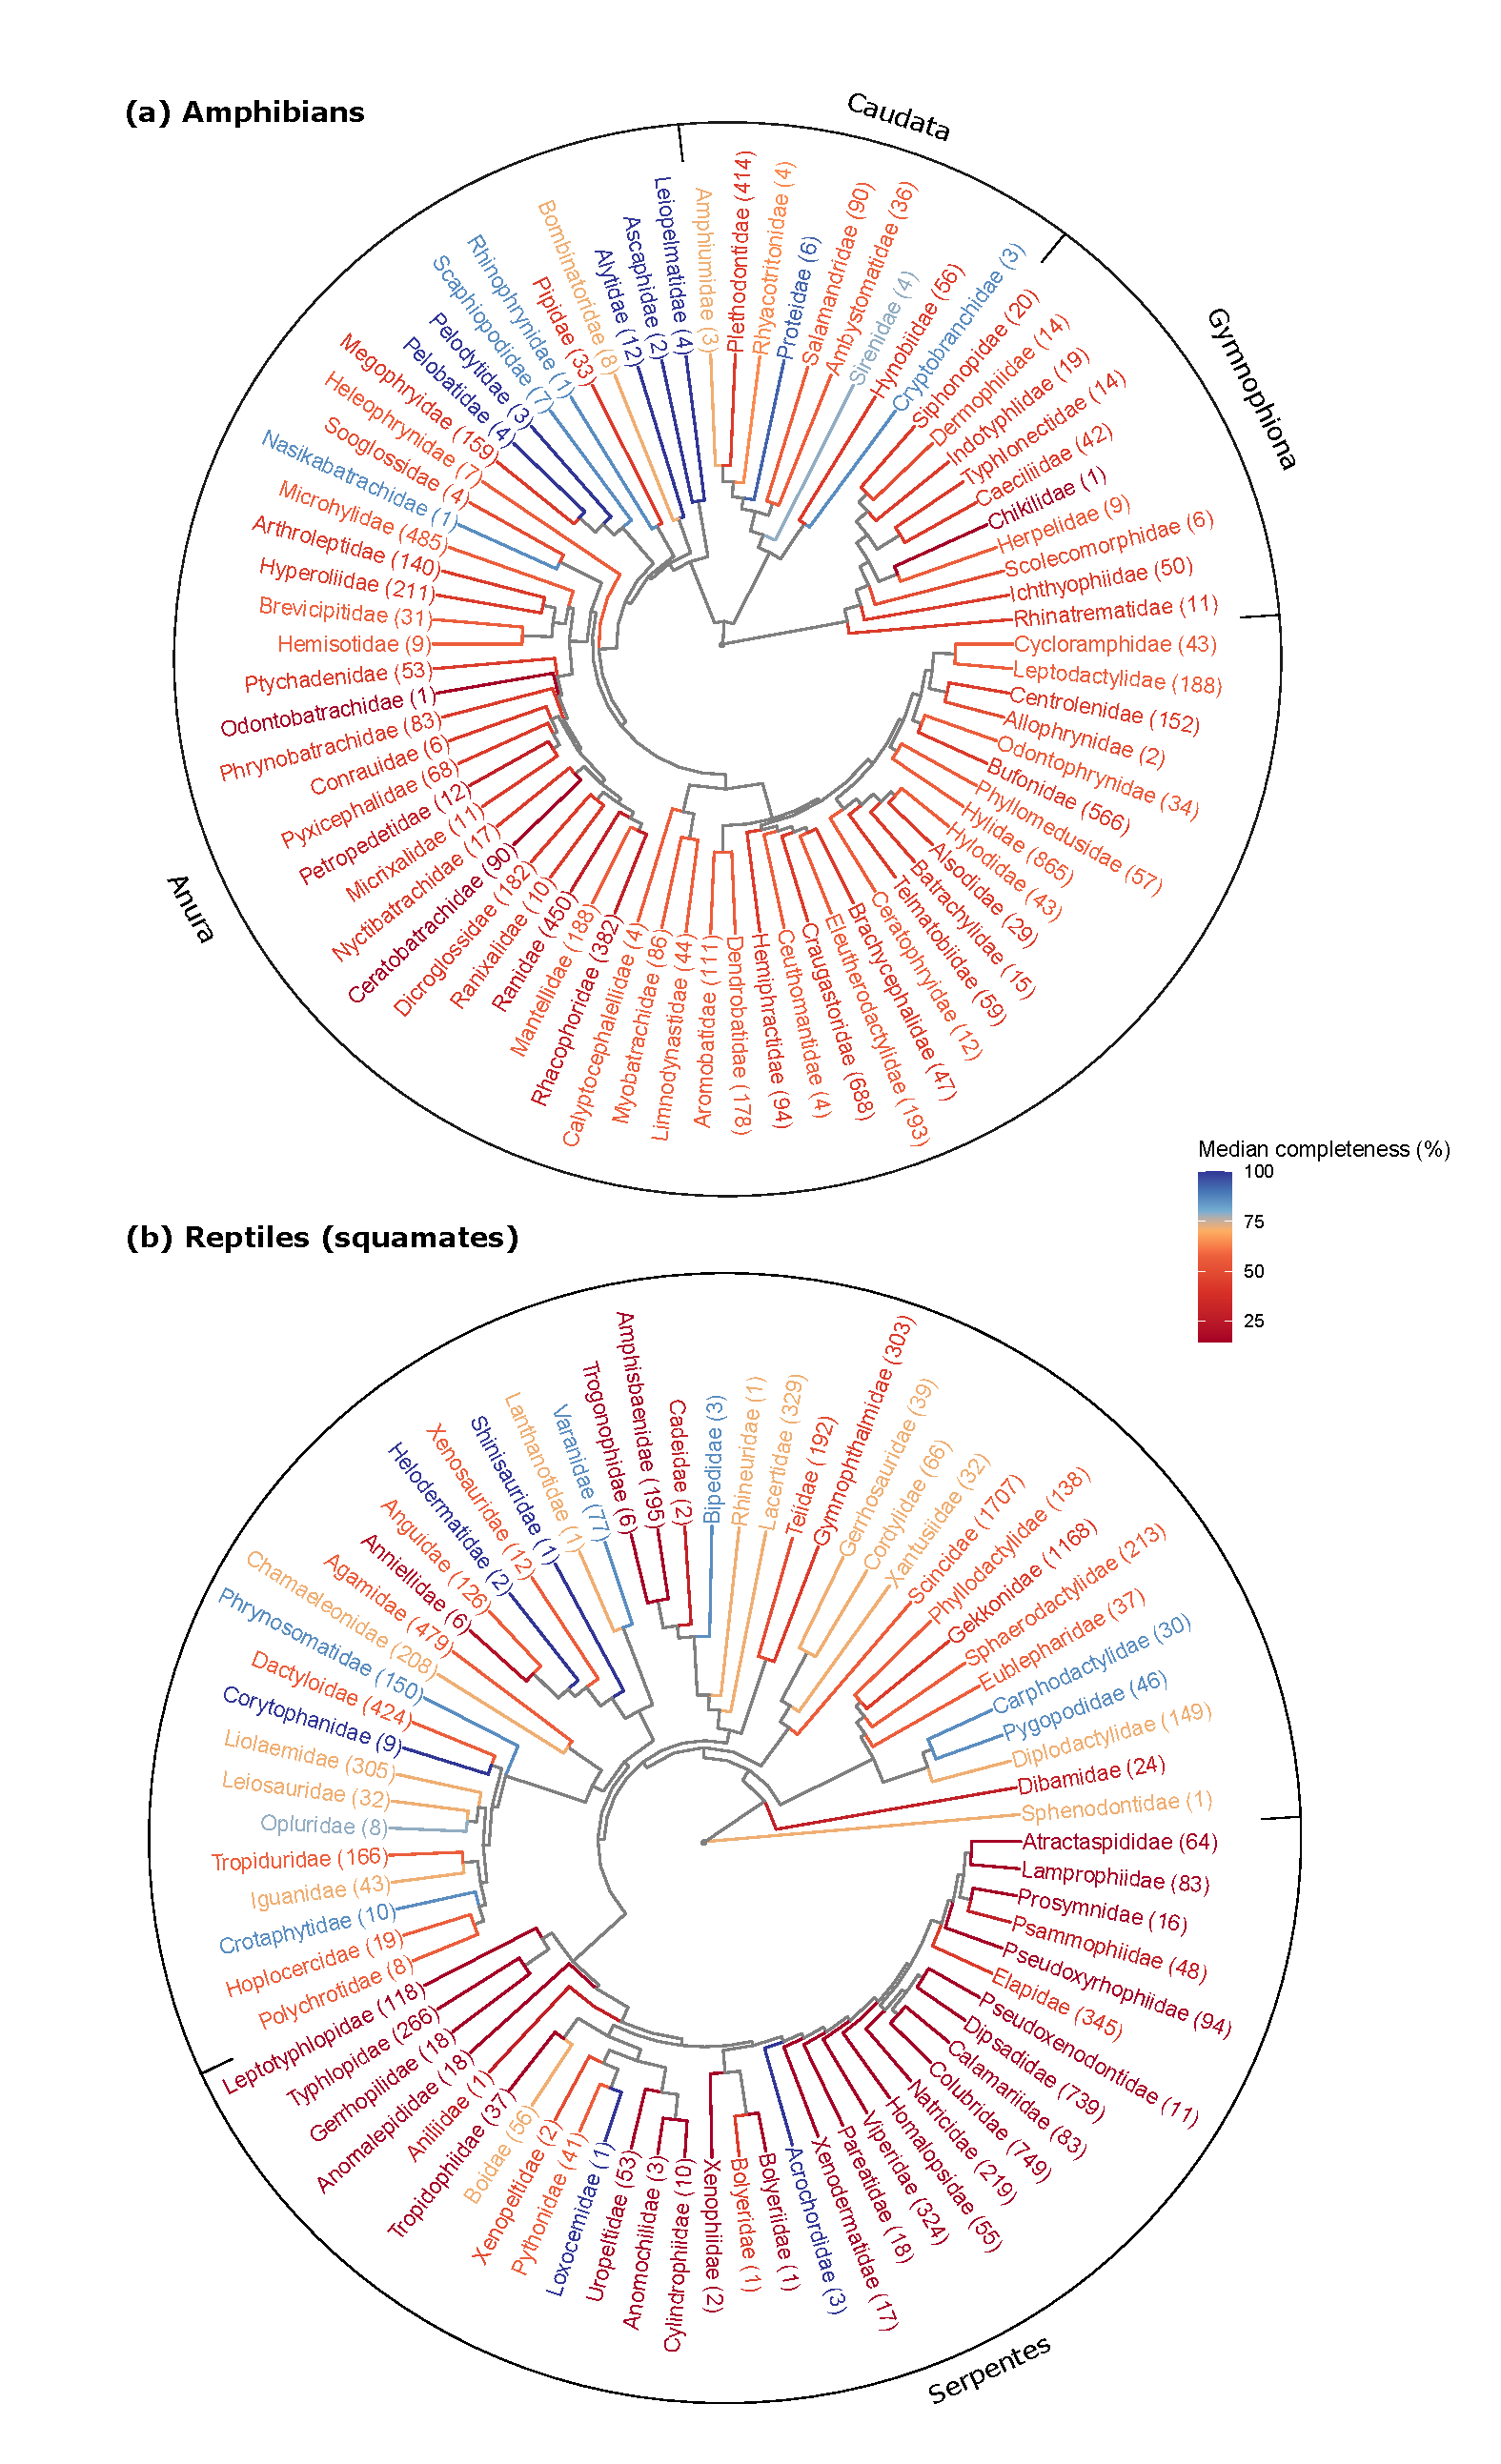
\includegraphics[scale=0.5]{figures/Chapter1/Figure_3}
\caption[Within-family median trait completeness in herptiles.]{\textbf{Within-family median trait completeness in herptiles.} The number next to each family name represents the number of species included in the calculation of the median.}
\label{1_Phylo}
\end{figure}

\clearpage

%% pick up the referencing to the SI figures here

\subsection{Spatial biases in trait completeness}
Range size was significantly correlated with the number of sampled traits. Larger range sizes were associated with a higher number of sampled traits (i.e., with higher completeness; Figure \ref{1_Range_size}; Supporting Information, Appendix 2, Table \ref{}). Similar results were obtained when using distribution maps not cut by elevational limits (Supporting Information, Appendix 2, Table \ref{}; Figure \ref{}). The rate of increase was steepest for reptiles, then for amphibians, then for birds and mammals (slope estimates for birds and mammals were not significantly different from each other; Supporting Information Table S1).

\begin{figure}[h!]
\centering
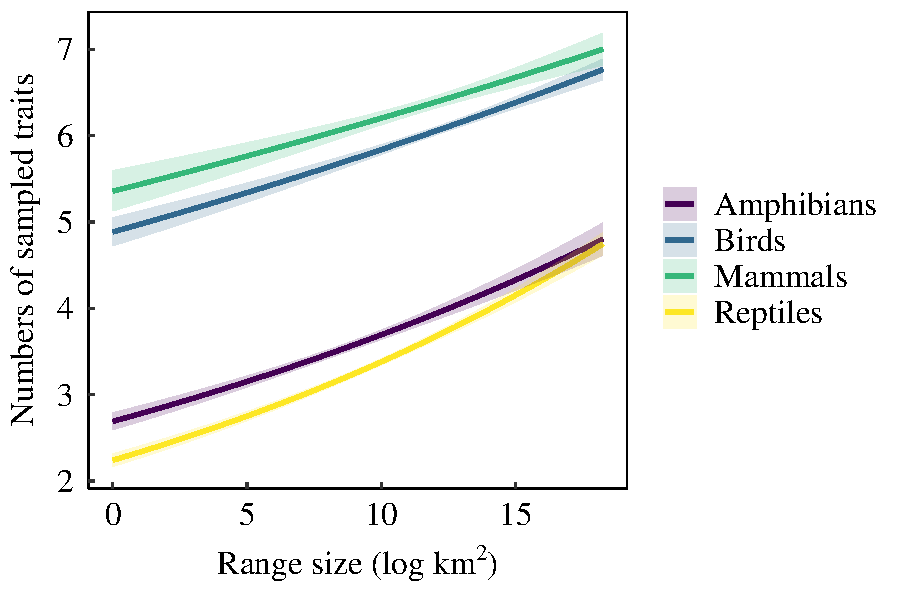
\includegraphics[scale=0.7]{figures/Chapter1/Figure_4}
\caption[Relationship between number of sampled traits and geographical range size]{\textbf{Relationship between number of sampled traits and geographical range size.} Models were fitted using a Poisson error distribution. Class was added as a predictor interacting with range size. Rates of increase in number of sampled traits with range size were not significantly different for mammals and birds but differed for reptiles and amphibians, with the steepest rates of increase for reptiles.}
\label{1_Range_size}
\end{figure}

There were marked spatial variations in median trait completeness in herptiles (Figure \ref{1_Map}). North America and Europe were well sampled for both amphibians and reptiles. Moreover, Southeast Asia and the Congo basin were on average less well sampled. In other regions, contrasting patterns emerged between amphibians and reptiles. For instance, median completeness was poorer for amphibians than for reptiles in Australia, but opposite patterns were observed in South America. As in the phylogenetic analyses, assemblage-level median completeness could mask potential important variation in completeness within species of a given assemblage. Assemblage-level mean and standard deviation maps are shown in the Supporting Information (Figures S8 and S9). There was a trend for increasing standard deviation with increasing species richness, with a larger spread in standard deviation at lower species richness (Supporting Information Figure S10).

\begin{figure}[h!]
\centering
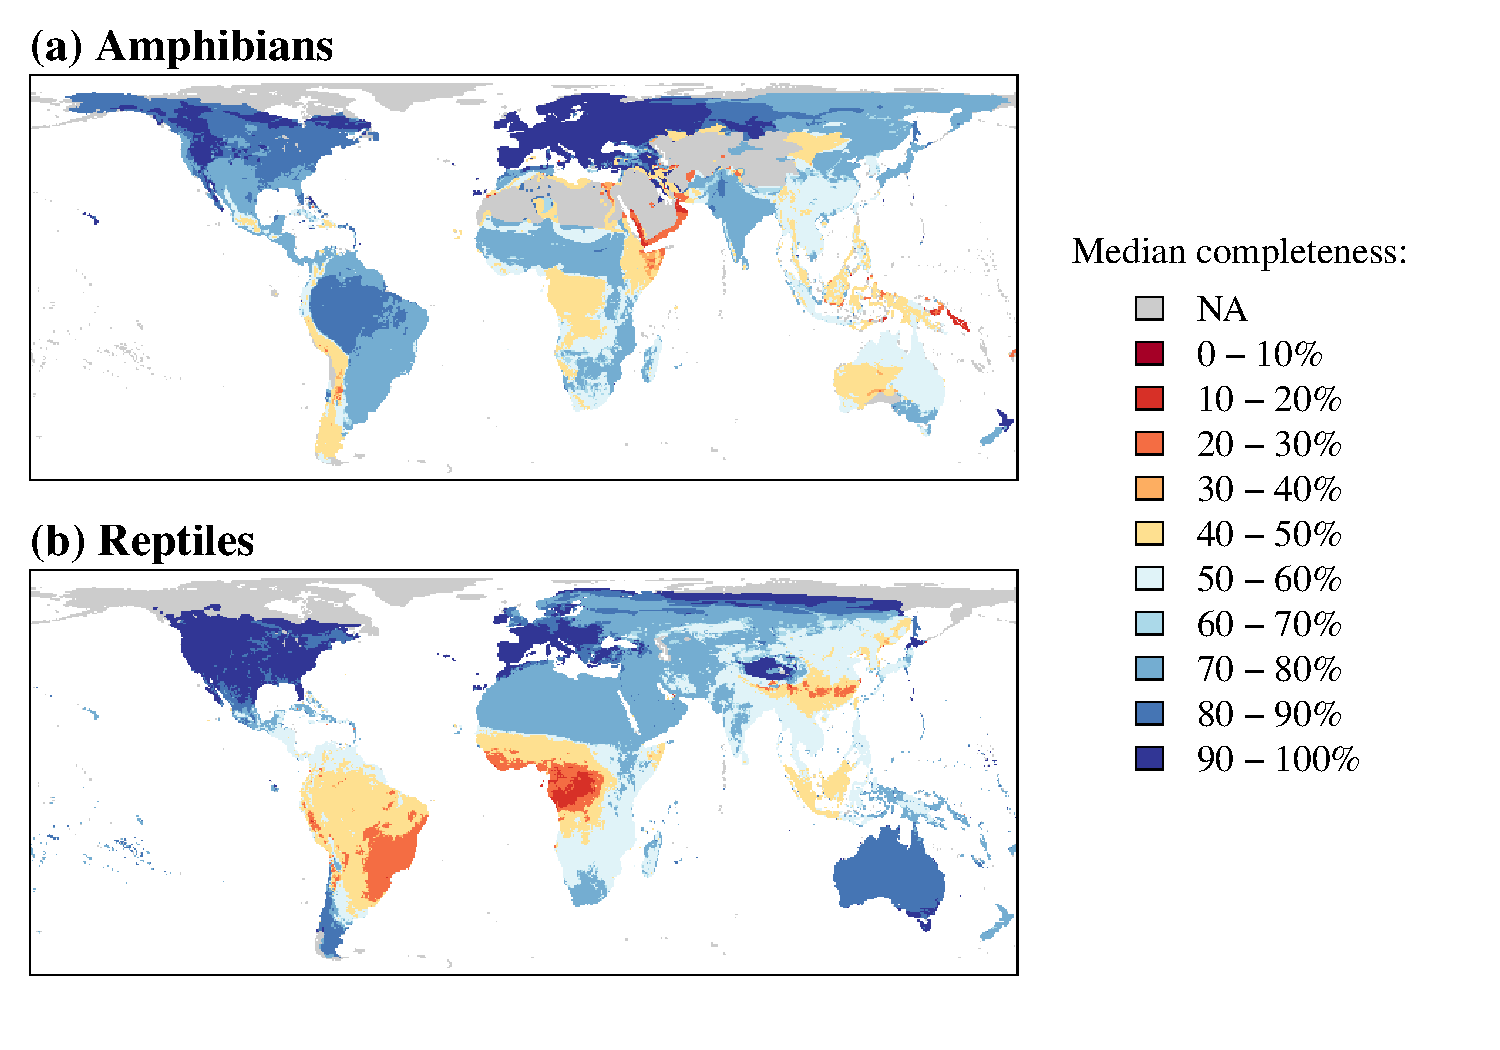
\includegraphics[scale=0.7]{figures/Chapter1/Figure_5}
\caption[Spatial distribution of assemblage-level median trait completeness in herptiles.]{\textbf{Spatial distribution of assemblage-level median trait completeness in herptiles.} Similar maps for birds and mammals are shown in the Supporting Information (Figure S7).}
\label{1_Map}
\end{figure}


Spatial models showed that species richness explained median trait completeness in herptiles in most realms (Figure 6; Supporting Information Tables S3 and S4); including spatial lags improved the models (reptiles: $\rho$ = 0.91, p-value < 0.0001; amphibians: $\rho$ = 0.92, p-value < 0.0001). For reptiles, completeness was negatively correlated with species richness in the most species-rich realms (Afrotropics, Indo-Malayan and Neotropics) and in the Palaearctic; the relationship was steepest in the Afrotropics and shallowest in the Palaearctic. In the Australasian and Nearctic realms, completeness tended to increase with species richness. For amphibians, negative relationships were observed in the Indo-Malay and Nearctic realms, whereas positive trends were observed in the Neotropics and the Palaearctic. The opposite trends between reptiles and amphibians observed in the Australasian and Neotropical realms reflected patterns observed on the maps. The Indo-Malayan was the only realm where median completeness tended to decrease with species richness for both reptiles and amphibians.

\clearpage
\begin{figure}[h!]
\centering
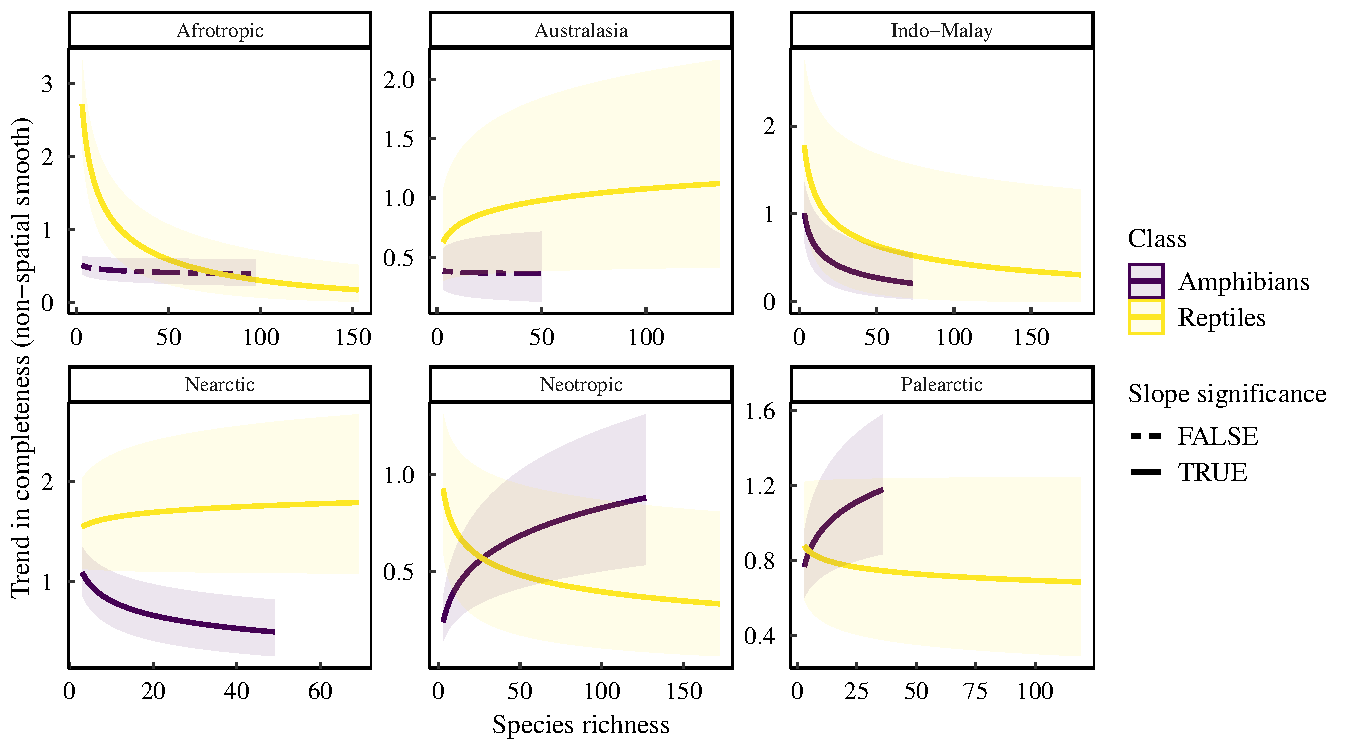
\includegraphics[scale=0.75]{figures/Chapter1/Figure_6}
\caption[Spatial model trends for herptiles.]{\textbf{Spatial model trends for herptiles.} The lines represent in-sample predictions ($\pm$ SE) for the trend components of the spatial models (trends after accounting for spatial autocorrelation).}
\label{1_Map}
\end{figure}


\section{Discussion}

The results of this chapter illustrate the taxonomic, spatial and phylogenetic dimensions of the knowledge gaps in trait data, termed the Raunkiæran shortfall by \citet{Hortal2015}. To the best of my knowledge, this work constitutes the first comparative assessment of global gaps for terrestrial vertebrate trait data, despite their use in numerous studies. I showed that the trait data present important taxonomic, spatial and phylogenetic biases, with contrasts in the availability of trait information between, on the one hand, herptiles and, on the other hand, birds and mammals.

Birds and mammals are globally well sampled for the set of traits I considered, even in the most species-rich assemblages. Moreover, the availability of trait information for herptiles is lower overall and phylogenetically and geographically biased. Several factors could interplay to shape these patterns. For instance, species that are more easily detectable (for example, wider ranging) and more charismatic are likely to be better sampled. Diverse socio-economic predictors could also contribute to geographical biases in trait data sampling; global biases in primary data collection are likely to be one of the most important contributors to the patterns I highlighted. Nevertheless, biases in the data could have been introduced at later stages, notably with the selection of sources and traits. The global compilation I obtained in this chapter reflects, in part, the interest and focus of the secondary data sources I used. It is possible that the addition of new sources from regional journals or other authorities could diminish spatial biases in the data by increasing coverage for certain areas. Nevertheless, I argue that by focusing on widely used traits, these results are likely to reflect the “true” availability of the data in primary sources and that the shortfalls for other, less used traits would be more pronounced.

I believe that the results presented here are robust to taxonomic uncertainty, although taxonomic matching might potentially be improved further using class-specific sources, such as the Reptile Database or AmphibiaWeb, for identification of synonyms (but see Supporting Information Appendix S9, Figure S16). I have made two versions of the data compilations available, one in which my own corrections were applied and one using the original binomial names of the sources, meaning that users are free to use their own taxonomic backbones and identify synonyms within the compilations.
I believe that taxonomic matching is a recurring issue when working across thousands of species. Taxonomic synonymy artefactually inflates the numbers of identified species, potentially lowering trait coverage (whereas clumping subspecies together can have the opposite effect). Tackling this problem is difficult \citep{Isaac2004, Jones2012}, notably because there is no global curated database recording the status of species names, and also because of the nature of taxonomy and the debates around the species concept \citep{May2011}. Nevertheless, taxonomic uncertainty can have important consequences. For instance, \citet{Cardoso2017} showed that inaccuracies and errors in species checklists contributed to the overestimation of plant diversity in the Amazon (but see \citet{Freeman2021}: the relative underdescription of species in tropical areas compared to temperate  areas (`taxonomic debt', also referred to as `latitudinal taxonomic gradient' by the authors) may lead to the underestimation of species richness at low latitudes).

Biases in trait data have important implications for conservation planning. Past studies have shown that narrow-ranged species, for which fewer trait data are available on average, have higher extinction risks \citep{Collen2016, Purvis2000, Ripple2017} and are more negatively impacted by anthropogenic pressures than wider-ranging species \citep{Newbold2018a}. Trait information is also less available for herptiles in tropical regions such as the Congo basin, Southeast Asia and South America, which are some of the most diverse areas of crucial importance for worldwide conservation \citep{Barlow2018}. Consequently, trait information is on average less available where potentially more crucial to conservation planning. Indeed, trait information can be incorporated into vulnerability assessments and, as such, can help to prioritize conservation efforts. Species traits have been found to mediate species responses to environmental changes across diverse taxonomic groups, and thus can inform on the sensitivity of species to anthropogenic pressures \citep{Flynn2009, Newbold2013, Nowakowski2017}. Traits are now commonly used to estimate species vulnerability or extinction risks \citep{Pacifici2015, RamirezBautista2020}. As opposed to trend-based approaches, which rely on historical population trends (changes in abundance or shifts in distributions) to predict species’ vulnerability and extinction risks, trait-based approaches rely on species’ intrinsic sensitivity to particular threats. The appeal of trait-based approaches to extinction risk estimation is that, by providing mechanistic insights, they diminish the amount of population information needed. If the responses of species to a threat consistently relate to certain traits, it is possible to generalize patterns across species for which population data are less available \citep{Verberk2013}. Integrating traits into vulnerability assessments is hence of particular interest when field monitoring of species population sizes or distributions is difficult to achieve, but biases in the data could mean that such information is lacking for some of the most vulnerable species.

%% 

Traits that influence species responses to environmental changes have been termed `response traits' (or `response-mediating traits'; \citet{Luck2012}), as opposed to `effect traits' that underpin ecosystem functioning \citep{Lavorel2002a}. For instance, relative brain size and longevity have been characterized as response traits in birds \citep{Newbold2013, Sayol2020}, whereas dietary characteristics (e.g., trophic levels or guilds) are both response and effect traits. \citet{Hortal2015} highlighted that, for plants, both response and effect traits have been investigated, whereas for vertebrates the research has been more focused on understanding species responses. This could be because the way vertebrate traits interact to shape some ecosystem processes has not yet been characterized well.

Ecosystem processes sustained by animals might be harder to quantify and might be influenced by a combination of traits. The traits compiled in this work are likely to have a role in diverse processes. Nevertheless, there was one important omission, in that I did not compile species diet in this chapter, potentially the most straightforward trait to link with diverse processes, such as grazing, pollination, scavenging and seed dispersal. From a practical perspective, I chose traits that had been estimated at least for some of the species in each class, and that were readily available. Diet was excluded because although estimates were available for amphibians, birds and mammals, there was no readily available database for reptilian diet. Movement or dispersal abilities were also excluded because information was not readily available for any class. Although I expect that species diet and dispersal abilities would present similar sampling biases to the ones presented in this work, the addition of such traits to the compilation would represent a valuable contribution and would notably facilitate studies looking at the functional roles of reptiles.

For practical reasons, I did not consider intraspecific trait variation. Intraspecific variation has been shown to have important effects on ecological systems, and a growing body of literature encourages trait-based research to include intraspecific variability \citep{Guralnick2016}. There have been several calls to produce open-access, global trait datasets \citep{Weiss2019}, including a representation of intraspecific trait variation \citep{Kissling2018}. Notably, \citet{Schneider2019} designed a framework to store and share inter- and intraspecific trait data, accompanied by an R package to standardize the data in a proposed format. Such a proposition could constitute an important step towards the unification of individual datasets into a single, comprehensive database for ecological trait data.

The current spatial and taxonomic gaps in trait data might limit our ability to scale studies up, whereas biases in the data can affect the validity of extrapolations to groups or areas that are undersampled. More generally, biases and gaps in biodiversity data can have important implications for ecological studies. Data gaps can hinder our ability to draw conclusions on observed macroecological patterns. For example, \citet{CHAUDHARY2016} proposed that marine species richness follows a bimodal distribution, peaking at mid-latitudinal locations, and argued that these patterns were not underpinned by knowledge gaps in species distributions. Nevertheless, \citet{Menegotto2018} attributed the tropical dip in marine species richness to a lack of species distribution data, explained by lower sampling efforts in tropical areas (`Wallacean' shortfall; \citet{Hortal2015}). Biases and gaps in trait data could also affect studies in closely related fields, such as functional ecology -- for instance, past studies have shown that functional diversity indices are sensitive to missing data \citep{Majekova2016, Pakeman2014} -- or community assembly \citep{Perronne2017}.

Ecologists should, therefore, take particular care when designing trait-based studies, because both data quality and data gaps are likely to influence the results and the generality of the conclusions. There exist diverse methods to deal with missing trait values, should data missingness be problematic. Complete removal of missing values (`case deletion') is commonly used but presents several issues, because it reduces sample size and statistical power and introduces potential bias in data subsamples \citep{Nakagawa2008}. For example, retaining complete cases only from the trait datasets would generate trait data disproportionally representative of mammals and birds, which would be problematic for conducting cross-taxon analysis on terrestrial vertebrates. As such, it is recommended that case deletion be applied only when data are missing completely at random, which is rarely the case \citep{Peugh2004}.

Alternatives to case deletion consist of filling in the gaps. In recent years, the development of imputation techniques has provided robust methods to handle missing data. Such imputation techniques have been used to complete trait datasets in recent studies \citep{Cooke2019b}. \citet{Penone2014} used a simulation approach to evaluate the performance of four of these techniques, namely PhyloPars \citep{Bruggeman2009}, random forest algorithms as implemented in R with missForest \citep{Stekhoven2016, Stekhoven2012}, multivariate imputation by chained equations (MICE; \citet{micepackage}) and k-nearest neighbour (kNN; \citet{Troyanskaya2001}). \citet{Penone2014} introduced missing values (10\%–80\%) in a complete trait dataset of carnivorans and measured imputation performance in different scenarios. Given that phylogenetic non-randomness in missing trait values can impact imputation accuracy, \citet{Penone2014} removed values in three different ways (completely at random; with a phylogenetic bias; and with a body mass bias). Out of the four techniques, missForest and PhyloPars performed best when species phylogenetic position was included as a predictor of missing trait values. Such imputations appeared to be robust even when trait coverage was as low as 40\%, which might be relevant for many reptilian and amphibian traits. The performance was not significantly affected by phylogenetic non-randomness of the data. Hence, missForest and PhyloPars appear to be well suited when traits are phylogenetically conserved, because they allow species phylogenetic position to be included as a predictor of missing trait values. The study by \citet{Penone2014} highlights that there are robust imputation techniques allowing to deal with incomplete trait data where biases might otherwise be problematic. Nevertheless, it is important to highlight that some imputation techniques, such as single or mean imputation, can be problematic because they do not allow an estimation of uncertainty and suffer from a lack of accuracy \citep{Nakagawa2008}; indeed, imputation techniques sometimes perform no better than case deletion. More work should be conducted to assess imputation performance in various contexts (see Johnson 2021), and the datasets compiled in this chapter might provide an opportunity for such studies.

%% Add Johnson ref for imputations??

Although robust imputation techniques can be useful for filling gaps in trait datasets, they are no substitute for continued data collection efforts. The results of this chapter show that data are particularly lacking in herptiles, notably in the Afrotropics, the Neotropics and the Indo-Malayan realms. For these areas, incorporating regional databases into existing datasets could contribute to the reduction of global gaps. I believe that both primary research and subsequent efforts to integrate new data and existing databases are required if we are to collectively strive towards the unification of trait databases.

To conclude, this work constitutes, to my knowledge, the first assessment of the global gaps and biases in terrestrial vertebrate trait information. I show that herptiles are undersampled compared with mammals and birds, with important spatial and phylogenetic variability in the availability of trait information. Imputation techniques are one possible solution to these problems. Nevertheless, I believe that primary research, combined with efforts to complete existing datasets, is the only way to fill the current data gaps genuinely and robustly. I hope that the compiled trait dataset and these findings can prove useful for guiding further data collection efforts and for conducting macroecological analyses.



\chapter{Different traits explain sensitivity to land use}
%%% chapter 3 Land use and functional diversity

\section*{Keywords}
Land use; land-use intensity; terrestrial vertebrates; functional diversity; traits.

\section*{Abstract}
Land-use change is the leading driver of global biodiversity loss, thus characterising its impacts on the functional structure of ecological communities is an urgent challenge. Using a database describing vertebrate assemblages in different land uses, I assess how the type and intensity of land use affect the functional diversity of vertebrates globally. I find that human land uses alter local functional structure by driving declines in functional diversity, with the strongest effects in the most disturbed land uses (intensely used urban sites, cropland and pastures), and among amphibians and birds. Both tropical and temperate areas experience important functional losses, which are only partially offset by functional gains. Tropical assemblages are more likely to show decreases in functional diversity that exceed those expected from species loss alone. These results indicate that land-use change non-randomly reshapes the functional structure of vertebrate assemblages, raising concerns about the continuation of ecological processes sustained by vertebrates.

\section{Introduction}
Anthropogenic activities are profoundly transforming global biodiversity. Although multiple pressures act in combination, land-use change currently poses the greatest threat to biodiversity \citep{Maxwell2016, Newbold2015}. However, not all species respond similarly to land-use change. Traits have been found to explain species' sensitivity to land-use change in diverse groups \citep{Newbold2013, Nowakowski2017, Quesnelle2014, Todd2017}. Previous work has also shown that land-use change leads to non-random modification of assemblage trait composition (or functional diversity) \citep{Chapman2018, Colin2018, Flynn2009, LaSorte2018, Newbold2013, Tinoco2018}. Since it is widely acknowledged that biodiversity, and in particular trait diversity, may promote ecosystem functioning and stability, modification to the trait composition of assemblages could have far-reaching and adverse impacts on ecological processes \citep{Hooper2012, Magioli2021, Oliver2015, Tilman1994}.

Terrestrial vertebrates support many processes, ranging from pollination \citep{Ratto2018}, to seed dispersal to the regulation of lower trophic levels \citep{Barber2010, Letnic2012, Salo2010,Zhang2018}. However, we lack a global understanding of how the functional diversity of entire vertebrate assemblages responds to changes in land use. Most previous studies have been conducted at regional or local scales \citep{Davison2021}, but these may not be representative of global patterns. Indeed, recent global syntheses have highlighted how biodiversity responses can differ substantially between regions and across latitudes, with higher sensitivity reported for the tropics \citep{Matuoka2020,Millard2021, Newbold2020}. Another key issue is the taxonomic coverage of past work. Few studies investigating effects of land use on functional diversity have considered several vertebrate classes together, and comparative studies remain rare. Thus, how land-use change affects the functional diversity of local vertebrate assemblages at global scales, and the potential geographical and taxonomic variation in the effects, still largely remains to be explored.

Here, I aim to assess how human land use and land-use intensity affect the functional diversity of vertebrate assemblages, across and within taxonomic classes. Building on recent work \citep{Matuoka2020,Millard2021, Newbold2020}, I investigate differences in response between tropical and temperate regions. I use multiple response metrics to quantify functional diversity. First, functional richness measures the breadth and variety of trait combinations represented in an assemblage \citep{Legras2018}. Second, functional dispersion quantifies how similar species in a given assemblage are in terms of their traits \citep{Laliberte2010}. These metrics can mask important alterations of assemblage composition if functional losses are compensated for by functional gains. To address this, I consider pairwise measures between assemblages, to explore levels of functional loss and functional gain across land uses (Figure \ref{chap3_fig1}).

%% Figure 1 %%

%%%%%%%%%%%%%%

To this end, I combine (1) the trait data across terrestrial vertebrates collected in Chapter 2 with (2) global records of species occurrence in eight land-use types of differing intensity of use (the PREDICTS database: \citet{Hudson2014, Hudson2017}; Figure \ref{chap3_fig1}; Appendix 2, Table \ref{SI3_Table1}). The PREDICTS database is currently the most comprehensive database of sampled species occurrence, and for most records also abundance, across multiple land uses of different land-use intensity. Using the PREDICTS database allows me to contrast biodiversity metrics among intact land uses (primary-vegetation sites, considered to be the undisturbed reference condition), and all other human land-use types. Specifically, I test the following hypotheses, both across and within taxonomic classes:

\begin{enumerate}
\item I expect decreases in functional diversity in human land uses compared to primary vegetation, caused by contractions of occupied trait space. I expect such effects to be more pronounced where land is used more intensively by humans. This hypothesis builds upon evidence that species with certain traits are more sensitive to land-use disturbance \citep{Newbold2013}, meaning that disturbed land uses will retain only disturbance-tolerant species, more functionally similar to one another. Given the reported higher sensitivity of tropical assemblages to land-use disturbance, I predict that such effects are stronger in the tropics.
\item I hypothesise that decreases in functional diversity in disturbed land uses exceed decreases expected by chance, given local species loss. Thus, I expect disturbed land uses to promote functional under-dispersion. Functional under-dispersion occurs when species within an assemblage are more similar, in term of their traits, than expected by chance \citep{Cadotte2017, Wong2018} -- or, in other words, when functional dispersion is lower than expected given local species richness. I predict that under-dispersion is more likely to occur in the highly disturbed sites, in both temperate and tropical areas. This hypothesis is based on the idea that species are being removed non-randomly from sensitive areas of the trait space, and increasingly so with higher disturbance level.
\item Finally, I expect decreases in functional diversity in human land uses to be driven by high functional loss, whereby species are being removed from previously occupied areas of the trait space; I expect no functional gain. This hypothesis is based on the idea that the functional trait space in undisturbed land uses represents all of the possible regional trait combinations and that species with functional attributes rendering them unable to persist in altered conditions will be filtered out \citep{Cornwell2006}.
\end{enumerate}

%% figure 1 - overview of study design and functional metrics
\begin{figure}[h!]
\centering
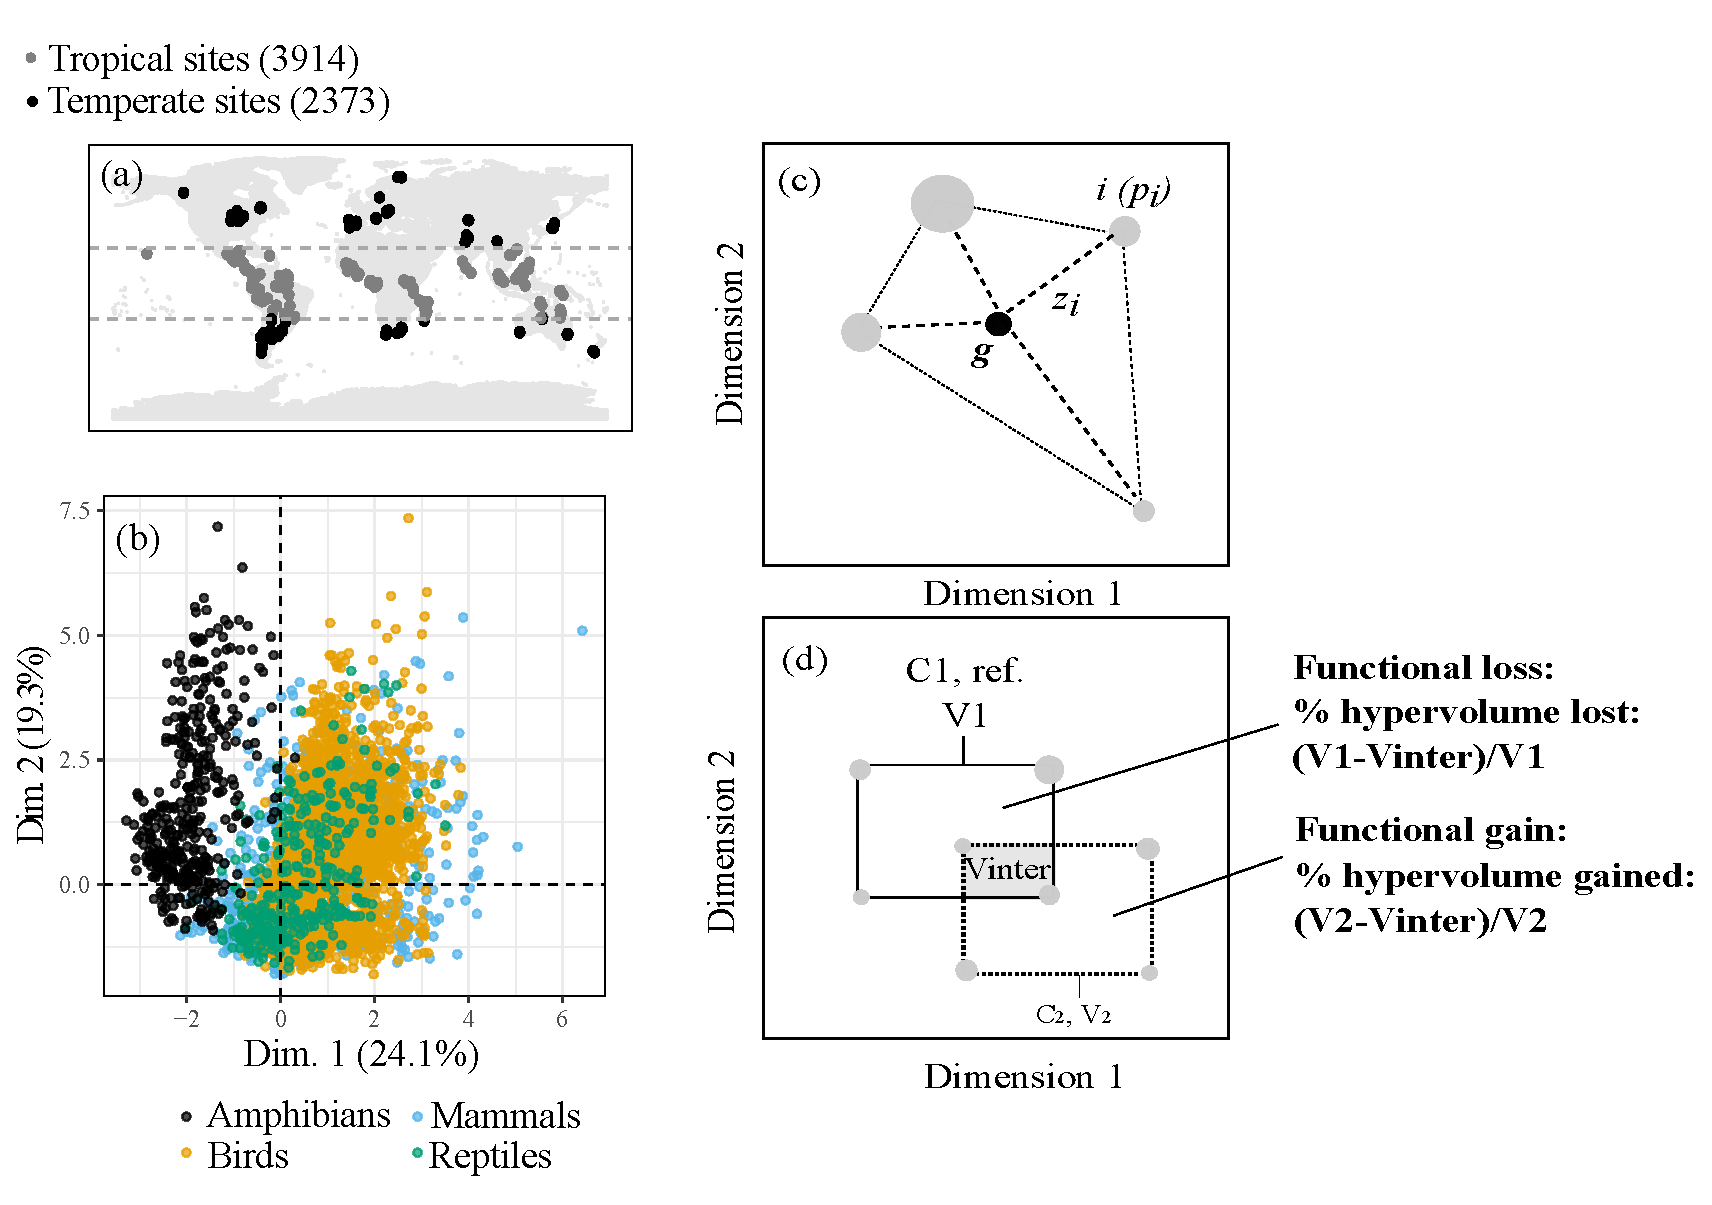
\includegraphics[scale=0.55]{figures/Chapter_FD/Figure1}
\caption[Overview of the study design and functional diversity metrics]{\textbf{Overview of the study design and functional diversity metrics.} I used occurrence data for vertebrate species from the PREDICTS database (\citep{Hudson2014, Hudson2017}; 180 studies; 431,170 records; 4,339 species; 6,758 sampled sites). \textbf{(a)} shows the spatial distribution of sites I consider. I combine occurrence data with trait data compiled in Chapter 2 to calculate functional diversity metrics. \textbf{(b)} is a representation of the trait data in two dimensions, plotted across PREDICTS vertebrates. Traits that contributed most to dimension 1 were lifespan (29\%) and litter/clutch size (22\%), while traits that contributed most to dimension 2 were habitat breadth (47\%) and use of artificial habitats (35\%). \textbf{(c)} and \textbf{(d)} present the conceptual framework for the calculation of the functional diversity metrics: local measures (c) and pairwise metrics (d). \textbf{(c)} Given a trait space, functional richness is calculated as the hypervolume occupied by the minimum convex hull encompassing all species \citep{Villeger2008}. Functional dispersion is calculated as the mean distance of the species to the centroid, \textbf{\textit{g}} \citep{Laliberte2010}. \textbf{(d)} I compute functional loss as the proportion of hypervolume lost from the reference assemblage, and I define functional gain as the proportion of hypervolume of the disturbed assemblage that was gained (proportion of novel trait space in the disturbed assemblage). \textit{Figure reproduced from \citet{Etard2021}.}}
\label{chap3_fig1}
\end{figure}



\section{Methods}

\subsection{Vertebrate assemblages}

I used vertebrate occurrence data from the PREDICTS database \citep{Hudson2014, Hudson2017}, a collection of studies that recorded species occurrence across multiple land uses and land-use intensities. In PREDICTS, each study contains several sites, which may be clustered into spatial blocks. Assemblage and land-use data are available at the site level: one site is characterised by a unique land use of given land-use intensity and provides occurrence data for a set of sampled taxa (and the same set of taxa is sought at all other sites within a study). Sites located between 23.5$^{\circ}$N and 23.5$^{\circ}$S of latitude were considered tropical, and otherwise temperate (Figure \ref{chap3_fig1}).

Land uses in PREDICTS were assigned to the following categories, based on the descriptions of the habitat given by the original collectors of the data: primary vegetation (considered to be the undisturbed reference); secondary vegetation; plantation forest; pasture; cropland; urban (considered human, or disturbed; Appendix 2, Table \ref{SI3_Table1};  \cite{Hudson2014, Hudson2017}). Secondary vegetation is further divided into three categories: mature, intermediate and young, depending on the stage of recovery of the vegetation. Land-use intensity is reported as minimal, light or intense, according to criteria that depended on the land-use type in question (e.g., crop diversity, degree of mechanisation and chemical inputs in cropland, or bushmeat harvesting and selective logging in primary vegetation; \cite{Hudson2014}). I excluded sites for which the land use could not be characterised or for which the stage of recovery of secondary vegetation was unclear. As the PREDICTS database is a collection of independent studies, the design of this study was not balanced: the sample size varied across land uses (Appendix 2, Figures \ref{SI3_F1} \& \ref{SI3_F2}), and across taxonomic groups (3,103 species of birds; 531 mammals; 379 amphibians; 326 reptiles).

\subsection{Functional traits and diversity metrics}
Trait choice is a critical step when calculating functional diversity metrics, which are highly sensitive to trait selection \citep{Mouillot2021}. However, trait selection trades off with data availability. Here, a constraint was to use similar traits across the different classes. %We chose seven traits from a compilation across terrestrial vertebrates \citep{Etard2020}, most of which are available for at least 50\% of the species in each class (except trophic level in amphibians and lifespan in herptiles [Figure S4]). 
Thus, I used the seven traits compiled in Chapter 2 across terrestrial vertebrates. Most of these traits were available for at least 50\% of the species in each class (except trophic level in amphibians and lifespan in herptiles; Appendix 2, Figure \ref{SI3_F4}). In addition, I chose traits that were ecologically relevant, broadening the biological definition of traits (i.e., a characteristic measurable at the level of an individual) to include measures of habitat breadth and habitat specialisation (still theoretically measurable at the level of an individual).  The final set constituted seven traits that influence species' responses to environmental change: body mass, trophic level, lifespan, litter/clutch size, diel activity, habitat breadth and use of artificial habitats. These traits related to life-history, habitat specialisation and use of geographical space (e.g., habitat breadth significantly explains geographical range size in all classes; Appendix 2, Figure \ref{SI3_F3}). Here, I did not consider estimations of dispersal abilities or home range size as these were available for a small fraction of the species ($<$3\%, \cite{AlexSmith2005, Paradis1998, Sutherland2000, Whitmee2013a}), neither did I include geographical range size which is measured across many individuals, and hence cannot be considered a trait. As in Chapter 2, I did not consider intraspecific trait variation, thus assuming no effect of the environment on trait values.

Trait coverage was variable among classes and traits, with important gaps for reptiles and amphibians (Appendix 2, Figures \ref{SI3_F4} \& \ref{SI3_F5}; Chapter 2). I imputed missing trait values using random forest algorithms (`missForest' package: \citet{Stekhoven2012}, \citet{Stekhoven2016}), including traits, taxonomic order and phylogenetic eigenvectors as predictors \citep{Debastiani2021, Penone2014}. To further assess the sensitivity of the results to imputation (see next section), I imputed missing trait values eight times, thereby obtaining eight sets of imputed traits. I randomly selected one imputed trait set for the calculation of functional metrics. Imputations of missing trait values \& imputation performance are detailed in Appendix 2, S3.2: `Trait data \& imputation of missing trait values' and S3.4: `Imputation performance' (and Figures \ref{SI3_F6}-\ref{SI3_F8}). Post-imputation, continuous traits were log$_{10}$-transformed (except habitat breadth which was square-rooted) and z-scored (standardised to unit variance and zero mean). In addition, I assessed whether the results were robust to imputation error using a subset of the PREDICTS data considering only species for which I had complete trait information (see next section).

Correlation among traits can be a safeguard against high sensitivity of functional metrics to trait omission, notably where omitted traits correlate strongly with traits that are already included in the calculation \citep{Mouillot2021}. Nevertheless, high multicollinearity among traits has been reported as potentially problematic for the calculation of functional diversity \citep{Cadotte2011}. Thus, I verified that the degree of multicollinearity among traits was not problematically high (with a threshold of 5 for variance inflation factors, Appendix 2, Table \ref{SI3_Table3}). Furthermore, I tested the sensitivity of the results to trait omission, by investigating whether adding geographical range size in the calculation of functional metrics was likely to affect the results.


\subsection{Effects of land use and land-use intensity on FRic and FDis (Hypothesis 1)}

For each assemblage, I measured functional richness using `FRic' \citep{Villeger2008}, and functional dispersion using `FDis’ (\citet{Laliberte2010}; Figure \ref{chap3_fig1}), from the `FD' package (\citet{Laliberte2010}; \citet{Laliberte2015}). I assessed the effects of land use, land-use intensity, and region (temperate versus tropical) on FRic and FDis across and within taxonomic classes using linear mixed-effects models (`lme4' package, \citet{Bates2015}). Land use and land-use intensity were not ranked in the models. A random intercept of study identity accounted for variation in experimental design across studies, while a random intercept representing spatial blocks of sampled sites, nested within study, accounted for spatial structuring within studies. To improve normality and bound predictions between 0 and 1, I transformed FRic and FDis using an arcsin-square-root transformation. The best-fitting model was sought using backwards stepwise model selection, starting with the most complex model that included all two-way interactions among the specified main effects. Model fits were compared using likelihood-ratio tests at each iteration of the selection procedure.

Across vertebrates, the starting models included the effects of land use, land-use intensity and region (temperate versus tropical). The best-fitting model for FRic was:
\pagebreak
\begin{center}
$\arcsin(\sqrt{\text{FRic}})\sim \text{Land use} + \text{Land-use intensity} + \text{Region} + \text{Land use}:\text{Land-use intensity} + \text{Land use}:\text{Region}$.\\
\end{center}
\hspace*{\fill}(Model 1a)

For FDis, the best-fitting model did not include interactions between land use and region, but the main effect of region was retained:
\begin{center}
$\arcsin(\sqrt{\text{FDis}})\sim \text{Land use} + \text{Land-use intensity} + \text{Region} + \text{Land use}:\text{Land-use intensity}$.\\
\end{center}
\hspace*{\fill}(Model 1b)

To investigate differences in responses across classes, I pooled some of the land uses together, because otherwise, sample sizes would have been too low. Mature, intermediate and young secondary vegetation were grouped together as `Secondary vegetation', and cropland and pasture were grouped together as `Agricultural land uses'. The starting models included the effects of land use, land-use intensity, region and taxonomic class. For FRic, the best model was:
\begin{center}
$\arcsin(\sqrt{\text{FRic}})\sim \text{Land use} + \text{Land-use  intensity} + \text{Region} + \text{Class} + \text{Land use}:\text{Land-use intensity} + \text{Land use}:\text{Class} + \text{Land-use intensity}:\text{Region} + \text{Class}:\text{Region}$.\\
\end{center}
\hspace*{\fill}(Model 2a)

For FDis, regional effects were dropped:
\begin{center}
$\arcsin(\sqrt{\text{FDis}})\sim \text{Land use} + \text{Land-use  intensity} + \text{Class} + \text{Land use}:\text{Land-use  intensity} + \text{Land use}:\text{Class} + \text{Land-use  intensity}:\text{Class}$.\\
\end{center}
\hspace*{\fill}(Model 2b)

To assess whether the results were robust to imputation error, I used a subset of the PREDICTS data considering only species for which there were complete trait information (6,212 sites; 442 mammals; 1,975 birds; 78 reptiles; 9 amphibians), and I fitted models again to this data subset. I did not have enough complete trait data among amphibians to be able to consider this class separately, so I first considered amphibians and reptiles together (herptiles), and reptiles only. In addition, I complemented this validation with a sensitivity analysis to variation in imputed values. I calculated FDis and FRic using each of the eight imputed trait datasets and fitted the previous models to each set. I then qualitatively evaluated the congruence of the estimates from the different models. Finally, because there tended to be more sites sampled in primary vegetation than in other land uses (Appendix 2, Figures \ref{SI3_F1} \& \ref{SI3_F1}), I ran additional sensitivity tests to assess whether the results were robust to resampling primary vegetation sites to a number equal to 50 (a sample size close to the median number of sites sampled in land uses other than primary vegetation in both regions (median = 37 for the temperate subset and 57 for the tropical subset, Appendix 2, Figure \ref{SI3_F1})).


\subsection{Investigating functional under-dispersion (Hypothesis 2)}

To assess whether effects of land use and land-use  intensity on FDis differed from what would be expected by chance given changes in local species richness, I generated null expectations of FDis at each site. I randomised assemblage composition 500 times, drawing species from the corresponding study's species pool while maintaining local species richness. For each site, I thus obtained a null distribution for FDis. Then, I tested whether FDis differed from null expectations using Wilcoxon signed-rank tests. I created a binary variable which was assigned 1 if FDis was significantly lower than null expectations at a given site (significant under-dispersion), and 0 otherwise. I investigated how land use, land-use intensity, region and taxonomic class affected the probability of occurrence of under-dispersion using a generalised linear mixed-effects model with a binomial distribution of errors. The best-fitting model did not retain any effect of taxonomic class:

\begin{center}
$\text{P\textsubscript{under-dispersion}} \sim \text{Land use} + \text{Land-use intensity} + \text{Region} + \text{Land use}:\text{Land-use intensity} + \text{Land use}:\text{Region}$.\\
\end{center}
\hspace*{\fill}(Model 3)

\subsection{Functional loss and functional gain (Hypothesis 3)}

I calculated the proportion of trait space that was lost in disturbed land uses compared to reference land uses (functional loss) and the proportion of trait space that was gained in disturbed land uses (functional gain) (Figure \ref{chap3_fig1}c), across and within taxonomic classes. I selected studies where at least one site was sampled in primary vegetation. I then made within study pairwise comparisons between reference assemblages, sampled in primary vegetation, and disturbed assemblages. In addition, I considered all comparisons between pairs of primary-vegetation sites, to create reference pairs. I then investigated how land use, land-use intensity and region affected functional loss and gain across and within taxonomic classes using linear mixed-effects models, controlling for study identity in the random effects. Across vertebrates, the best-fitting model for functional loss was:

\begin{center}
$\arcsin(\sqrt{\text{loss}})\sim \text{Land use} + \text{Land-use intensity} + \text{Region} + \text{Land use}:\text{Land-use intensity} + \text{Land use}:\text{Region}$.\\
\end{center}
\hspace*{\fill}(Model 4a)

For functional gain, one interaction term (land use with region) was dropped:

\begin{center}
$\arcsin(\sqrt{\text{gain}})\sim \text{Land use} + \text{Land-use intensity} + \text{Region} + \text{Land use}:\text{Land-use intensity}$.\\
\end{center}
\hspace*{\fill}(Model 4b)

When considering the effects of taxonomic class, the best-fitting model for functional loss was:
\begin{center}
$\arcsin(\sqrt{\text{loss}})\sim \text{Land use} + \text{Land-use intensity} + \text{Class} +\text{Region} + \text{Land use}:\text{Land-use intensity} + \text{Land use}:\text{Class} + \text{Land use}:\text{Region} + \text{Land-use intensity}:\text{Class}$.\\
\end{center}
\hspace*{\fill}(Model 5a)

For functional gain (Model 5b), the fitted effects were the same as those of Model 2b. More details about the calculation of functional loss and gain can be found in Appendix S3.5.

All data analyses were conducted using R version 3.5.1 (R Core Team, 2018). I made the code available on figshare (DOIs: \url{https://doi.org/10.6084/m9.figshare.14161883} and \url{https://doi.org/10.6084/m9.figshare.15163926}), as well as the main result datasets (\url{https://doi.org/10.6084/m9.figshare.15163971}).

\section{Results}

\subsection{Effects of land use on FRic and FDis}

Across all vertebrates, land use and land-use intensity significantly affected FRic and FDis (Figure \ref{chap3_fig2}). FRic tended to decrease with increasing disturbance level and higher intensity of land use. For FRic, relative effects differed between regions (Figure \ref{chap3_fig2}a). Although declines were overall more important for disturbed tropical assemblages, significant declines were observed for the temperate assemblages (e.g., a 37\% average decline in intensely used urban areas; a 49\% decline in pastoral areas of high land-use intensity). Nevertheless, tropical assemblages typically showed more important reductions in FRic. For instance, declines averaged 63\% for intensely used tropical cropland and 76\% for urban areas. For FDis, relative effects were similar in both regions (Figure \ref{chap3_fig2}b). The most important average declines were observed for urban assemblages of intense use (20\% decline), and for lightly- and intensely used cropland (by 15\% and 26\%). Note that confidence intervals around the estimated average declines were large in some cases, highlighting some heterogeneity in the responses.

%% figure 2 
\begin{figure}[h!]
\centering
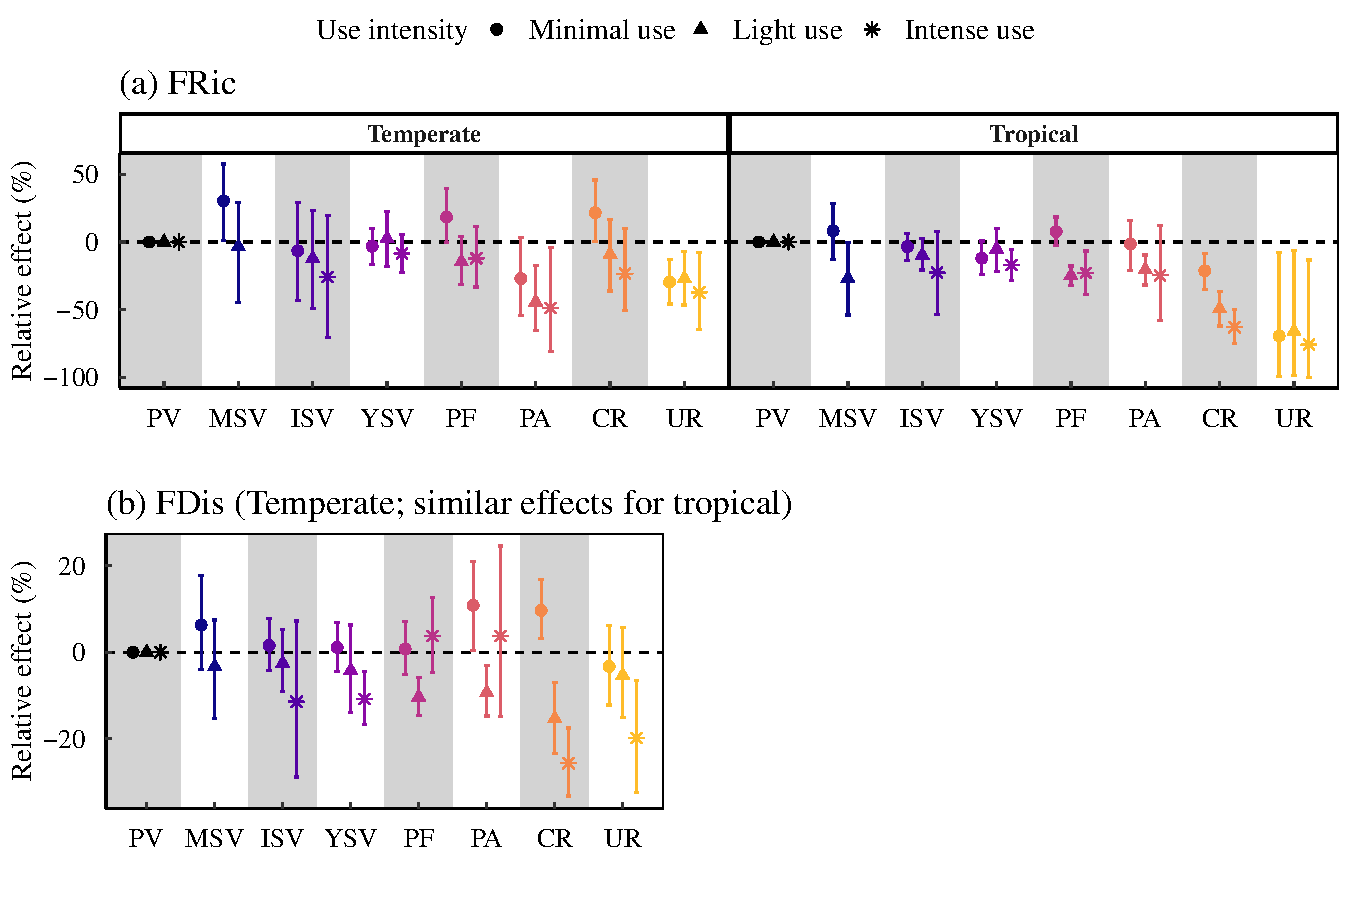
\includegraphics[scale=0.75]{figures/Chapter_FD/Figure2}
\caption[Effects of land use, land-use intensity and region on FRic (a) and on FDis (b) across all PREDICTS vertebrates.]{\textbf{ Effects of land use, land-use intensity and region on FRic (a) and on FDis (b) across all PREDICTS vertebrates.} Effects were rescaled with reference to primary vegetation (PV) and are plotted as a \% difference relative to PV within each land-use intensity. For FRic, the best-fitting model included interactions between land use and region, while these interactions were dropped for FDis, explaining the similar relative effects in both regions. Error bars represent 95\% confidence intervals. MSV: mature secondary vegetation; ISV, intermediate secondary vegetation; YSV, young secondary vegetation; PF, plantation forest; PA, pasture; CR, cropland; UR, urban. Effects for intense use in MSV could not be estimated as there were not enough sampled sites. \textit{Figure reproduced from \citet{Etard2021}.}}
\label{chap3_fig2}
\end{figure}

Fitting the same models to the subset of species with complete trait data, I detected important declines in functional diversity in a number of land uses, showing that the conclusions are robust to trait imputation uncertainty (for example, FRic declined on average by 75\% in intensely used temperate pastoral assemblages; by 48\% for intensely used tropical cropland; and FDis declined by an average 37\% in intensely used tropical urban assemblages; Appendix 2, Figure \ref{SI3_F18}). Furthermore, using the subset of species with complete trait data, I found that the results were not sensitive to the inclusion of geographical range size as an additional trait (Appendix 2, Figure \ref{SI3_F19}). Finally, the results were not sensitive to variation across imputed trait values (Appendix 2, Figure \ref{SI3_F20}) and were also robust to resampling in primary-vegetation sites (Appendix 2, Figure \ref{SI3_F21}).

Responses of FRic and FDis to land use and land-use intensity differed among taxonomic classes (Figure \ref{chap3_fig3}). Within-class effects for FDis were similar between regions. The most notable decreases were observed in lightly- and intensely used agricultural land uses in amphibians, birds and reptiles; and in intensely used urban land uses for birds and mammals. For FRic, the effects in tropical and temperate regions were qualitatively similar in three out of four classes (birds, mammals and reptiles), although effect sizes tended to be bigger for tropical assemblages. Birds and reptiles showed reductions in disturbed land uses in both tropical and temperate regions, whereas I detected few significant effects for mammals. For birds, the most important average decline, of 50\%, was observed in intensely used tropical urban land uses, while for reptiles I detected significant decreases in lightly- and intensely used agricultural sites (but I could not estimate effects for urban land uses due to the small sample size). Finally, the effects differed between tropical and temperate regions for amphibians, with no significant effects detected across temperate assemblages, but important reductions across tropical agricultural and urban assemblages.

%% figure 3
\begin{figure}[h!]
\centering
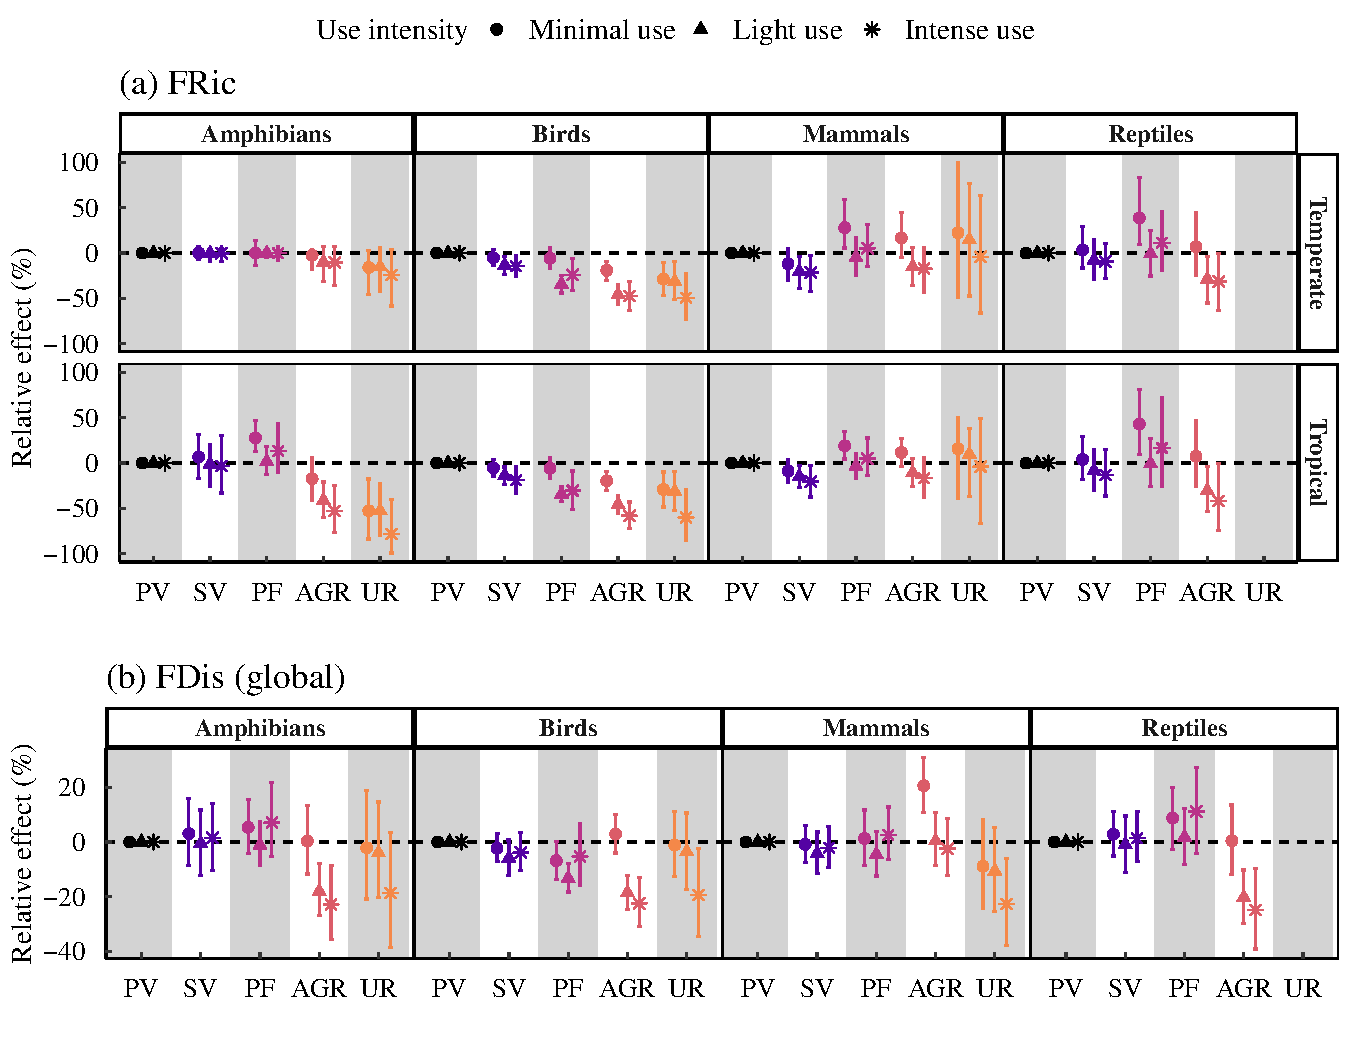
\includegraphics[scale=0.75]{figures/Chapter_FD/Figure3}
\caption[Effects of land use, land-use intensity, region and taxonomic class on FRic (a) and FDis (b).]{\textbf{Effects of land use, land-use intensity, region and taxonomic class on FRic (a) and FDis (b).} Effects were rescaled with reference to primary vegetation (PV) and are plotted as a \% difference relative to PV within each land-use intensity. Error bars represent 95\% confidence intervals. Effects for FRic were estimated from Model 2a, and from Model 2b for FDis. SV, secondary vegetation; PF, plantation forest; AGR, agricultural land uses (pasture and cropland); UR, urban. Effects for reptiles in urban land uses could not be estimated as there were not enough sampled sites. \textit{Figure reproduced from \citet{Etard2021}.}}
\label{chap3_fig3}
\end{figure}

Fitting similar models only for species with complete trait data showed that these patterns are unlikely to be affected by imputation uncertainty for birds; for mammals and reptiles, the main results could even be conservative (Appendix 2, Figures \ref{SI3_F22}, \ref{SI3_F23}). Indeed, although confidence intervals around the estimates were large, I typically observed larger decreases in functional diversity when using the complete data subset, including an 86\% decline in FRic for mammals in intensely used tropical agricultural areas. The results were also unaffected by variation across replicate sets of imputed trait values (Appendix 2, Figure \ref{SI3_F24}).

%\clearpage

\subsection{Changes in the probability of occurrence of functional under-dispersion}

Land use, land-use intensity and region significantly affected the probability of occurrence of functional under-dispersion across vertebrates. Functional under-dispersion was more likely to occur in tropical cropland of all land-use intensities (Figure \ref{chap3_fig4}b), as well as in some of the lightly-used land uses (notably urban and plantation forest). Contrary to my expectations, and with the exception of tropical cropland, functional under-dispersion was not more likely to occur in intensely-used land uses. For minimally-used sites, changes in FDis were mostly consistent with changes expected given local species richness.

%% figure 4
\begin{figure}[h!]
\centering
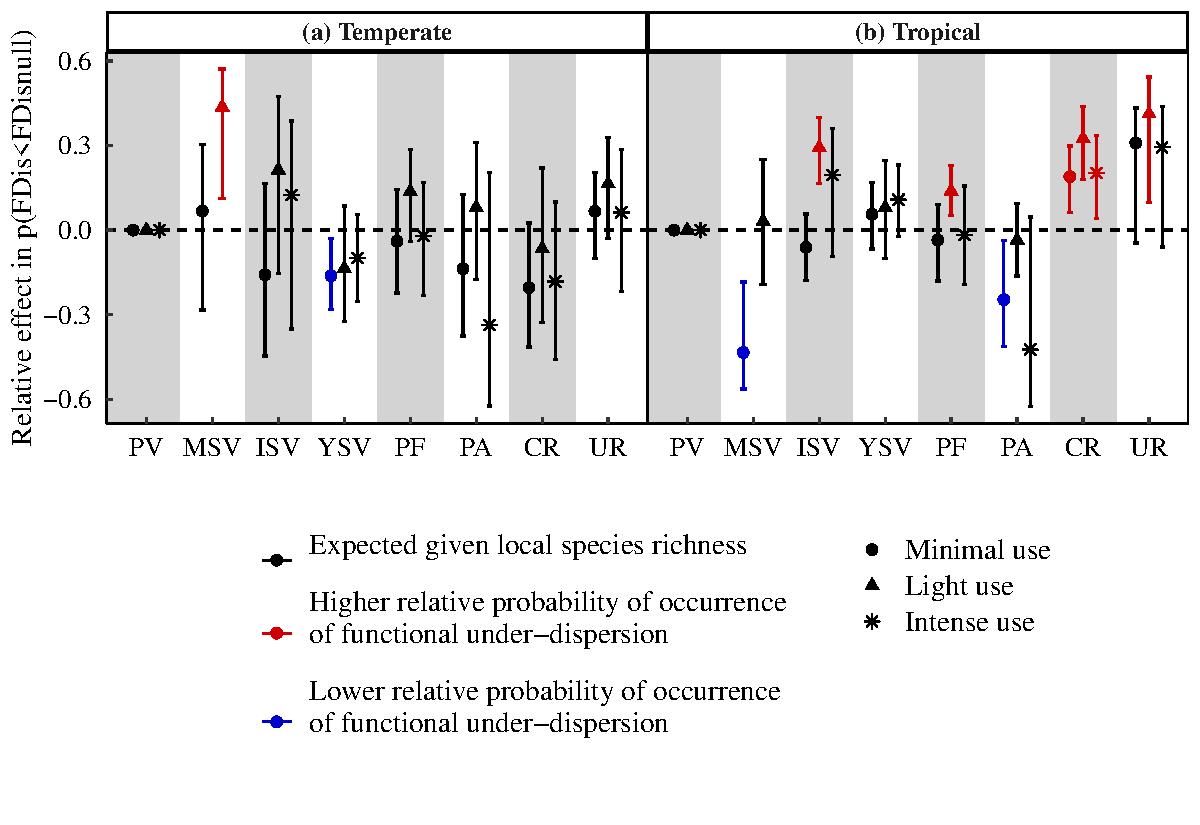
\includegraphics[scale=0.75]{figures/Chapter_FD/Figure4_new}
\caption[Effects of land use, land-use intensity and region on the probability of occurrence of functional under-dispersion.]{\textbf{Effects of land use, land-use intensity and region on the probability of occurrence of functional under-dispersion.} Error bars represent 95\% confidence intervals. PV: primary vegetation; MSV, mature secondary vegetation; ISV, intermediate secondary vegetation; YSV, young secondary vegetation; PF, plantation forest; PA, pasture; CR, cropland; UR, urban. Effects are rescaled and represent the average difference in the probability of occurrence of functional under-dispersion between the reference (PV, probability of functional under-dispersion set at 0 within each land-use intensity) and the disturbed land uses. \textit{Figure reproduced from \citet{Etard2021}.}}
\label{chap3_fig4}
\end{figure}

\subsection{Functional loss and gain}

Across and within vertebrate classes, I detected high levels of functional loss, exceeding the natural turnover between primary-vegetation sites, both in temperate and tropical regions. Across vertebrates (Figure \ref{chap3_fig5}a), functional loss was notably high in temperate pastures (+27\% above reference for minimal use; +73\% for intense use), temperate urban sites (+27\% for light use; +50\% for intense use; effects for tropical urban sites could not be estimated), temperate and tropical cropland (+44\% and +56\% respectively for light use; effects for intense use could not be estimated). Important levels of functional loss were also observed in tropical plantation forest of light use intensity (+51\%; effects for the intense use could not be estimated). High levels of functional loss were also observed within each class (Figure \ref{chap3_fig6}a) (although not all effects could be estimated because of limited sample sizes, Appendix 2, Table \ref{SI3_Table5}). The highest losses were observed in agricultural areas for amphibians and reptiles, with important losses also observed in temperate urban areas for both birds and amphibians (+35\% for minimal use; effects for tropical urban areas could not be estimated).

%% figure 5
\begin{figure}[h!]
\centering
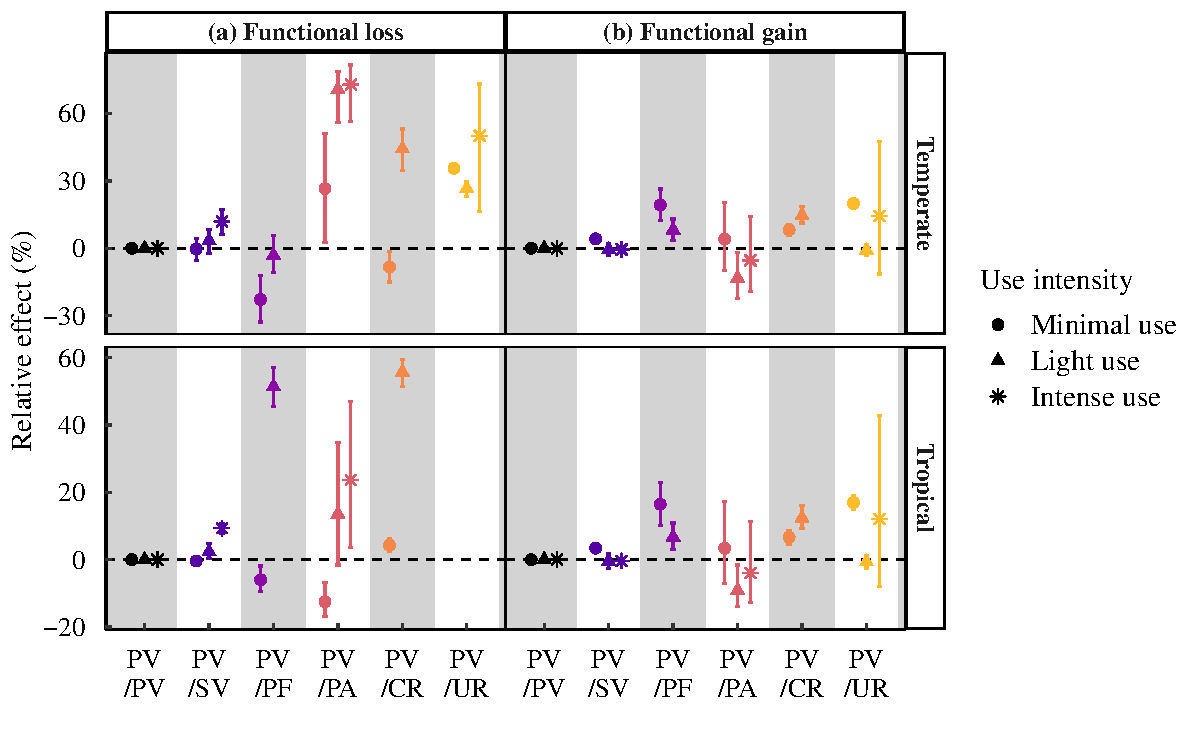
\includegraphics[scale=0.75]{figures/Chapter_FD/Figure5}
\caption[Effects of land use and land-use intensity on (a) functional loss and (b) functional gain across pairs of sites in temperate areas and tropical areas.]{\textbf{Effects of land use and land-use intensity on (a) functional loss and (b) functional gain across pairs of sites in temperate areas and tropical areas.} PV: primary vegetation; SV, secondary vegetation; PF, plantation forest; PA, pasture; CR, cropland; UR, urban. Error bars represent 95\% confidence intervals. Effects are rescaled and represent the average difference in functional loss and gain between the reference pairs (PV/PV, with loss and gain set at 0\% within each land-use intensity), and pairs of primary vegetation with disturbed land uses. Negative effects mean that, on average, levels of functional loss (or gain) were lower than functional loss (or gain) observed between pairs of primary-vegetation sites, and not that there were absolute `negative losses' or `negative gains'. \textit{Figure reproduced from \citet{Etard2021}.}}
\label{chap3_fig5}
\end{figure}

Across vertebrates, average functional gain (average proportion of novel trait space in the disturbed assemblage) was moderate and on average did not exceed 20\% in any disturbed land uses (Figure \ref{chap3_fig5}b). Patterns of functional gain were similar in both regions. The highest functional gains were observed for minimally-used urban sites and plantation forest (range: +16\% to +20\%). On the other hand, important levels of functional gain were observed in some classes (Figure \ref{chap3_fig6}b), with the highest functional gain for mammals (+80\% in intensely used urban sites).

Diagnostic plots (qq-plots and residual distributions) for the models are shown in Appendix 2, Figures \ref{SI3_F9}–\ref{SI3_F17}. Overall, the model residuals were appropriately distributed (but with some leptokurtic residual distributions, to which mixed-effect models are generally robust \citep{Schielzeth2020}).

%% figure 6
\begin{figure}[h!]
\centering
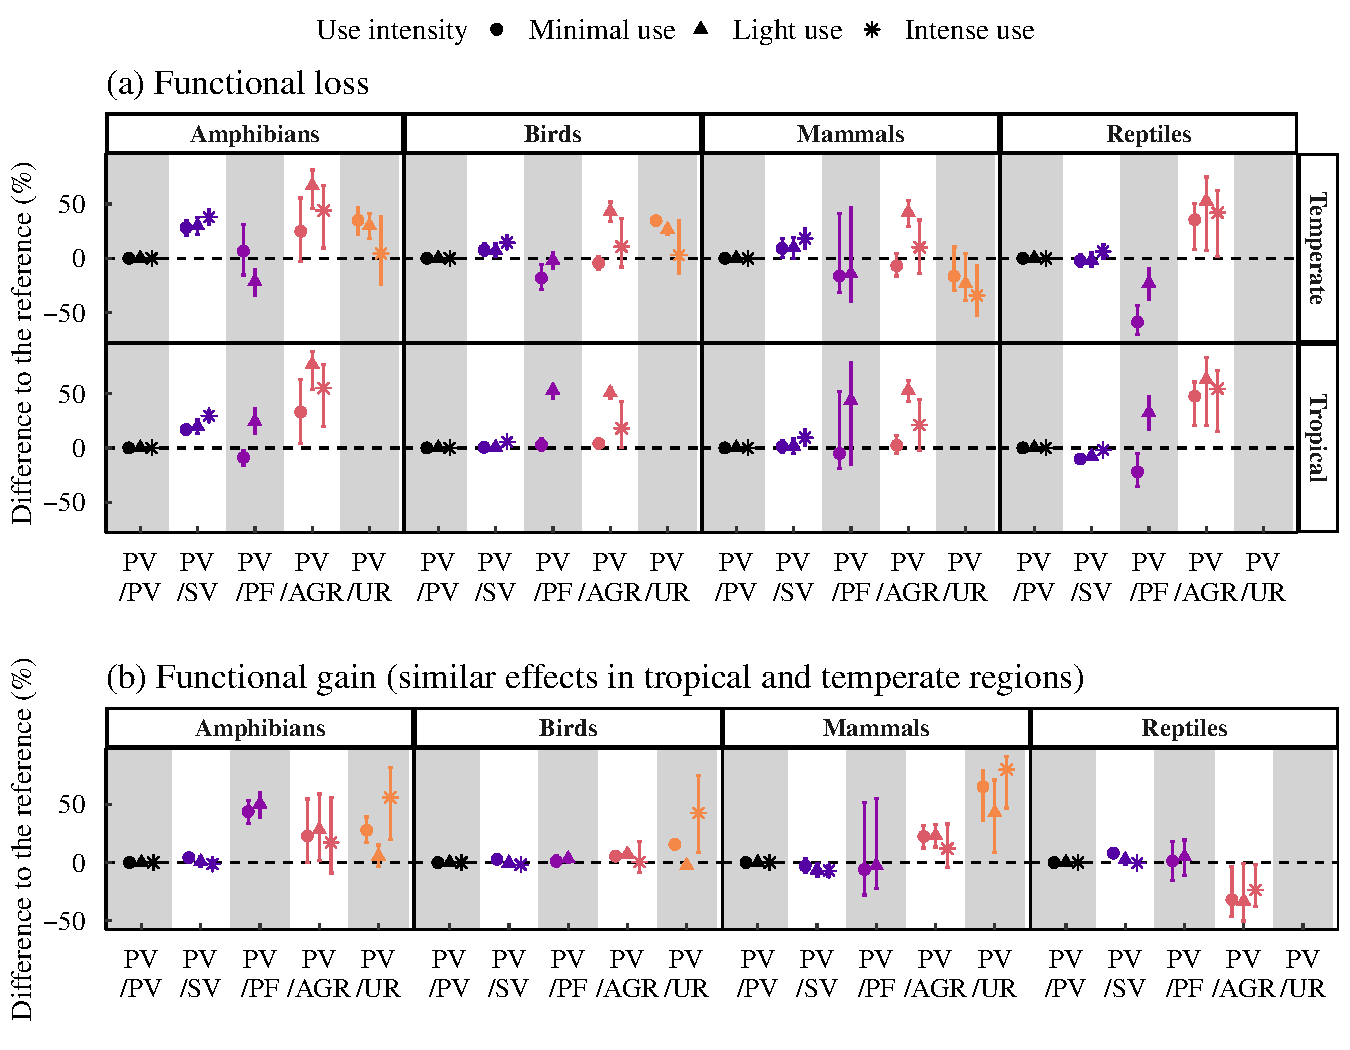
\includegraphics[scale=0.75]{figures/Chapter_FD/Figure6}
\caption[Effects of land use, land-use intensity, region and taxonomic class on functional loss and functional gain across pairs of sites.]{\textbf{Effects of land use, land-use intensity, region and taxonomic class on functional loss (a) and functional gain (b) across pairs of sites.}  PV: primary vegetation; SV, secondary vegetation; PF, plantation forest; AGR, agricultural land uses (pasture and cropland); UR, urban. Error bars represent 95\% confidence intervals. Effects are rescaled and represent the average difference in functional loss and gain between the reference pairs (PV/PV, with loss and gain set at 0\% within each land-use intensity), and pairs of primary vegetation with disturbed land uses. Negative effects mean that, on average, levels of functional loss (or gain) were lower than functional loss (or gain) observed between pairs of primary-vegetation sites, and not that there were absolute `negative losses' or `negative gains'. \textit{Figure reproduced from \citet{Etard2021}.}}
\label{chap3_fig6}
\end{figure}

\clearpage
\section{Discussion}
Here, I showed that the functional diversity of vertebrate assemblages is negatively impacted in human land uses, particularly in the most intensely used land types. The results of this Chapter extend previous studies that have been more taxonomically or geographically restricted \citep{Flynn2009, Matuoka2020}. \citet{Matuoka2020} found that the functional diversity of tropical bird assemblages was negatively affected by human disturbance, a pattern that did not appear in temperate assemblages. Yet, I found that functional diversity was negatively affected in both tropical and temperate areas, with important functional losses in all four vertebrate classes.

Using multiple metrics allowed me to explore different facets of functional diversity. For instance, functional gain could locally offset functional loss in some disturbed land uses. This could indicate that despite no apparent negative effect on FRic, some disturbed land uses (e.g. lightly-used temperate cropland) could experience important functional loss, and highlights the importance of using a variety of indicators. This mechanism could be at play in mammalian assemblages, for which important levels of functional gain were observed in agricultural and urban sites. Further, functional gain in disturbed land uses could indicate that disturbances facilitate the introduction of functionally novel species, falling into previously unoccupied parts of the trait space. This may be because non-native species are more likely to become established in disturbed assemblages. Previous work has shown that land-use disturbance facilitates biological invasions in island ecosystems \citep{Jesse2018,Sanchez-Ortiz2019}, but to my knowledge, this has not been tested specifically across continental areas for invasive vertebrates (but see \citet{Pysek2010}). It is also possible that disturbed areas harbour synanthropic species that do not occur in primary vegetation, leading to substantial functional gain.

Overall, the negative effects of land use on functional richness tended to be more pronounced in the tropics. This is congruent with past studies that have found tropical biodiversity to be disproportionally sensitive to human pressures \citep{Newbold2020, Martins2017}. There are a number of potential explanations for this. First, it could be that a long history of intense land-use disturbance at large scales in many temperate regions (e.g. Western Europe; \citet{Stephens2019}) means that biodiversity is now less sensitive to new disturbances, because the most sensitive species have been filtered out \citep{Balmford1996, Krauss2010, LeProvost2020, Munteanu2020}. Species unable to cope with such disturbances may have gone extinct in the past, while the remaining species would be more disturbance-tolerant \citep{Betts2019}. Tropical regions, historically less disturbed at large scales, would then contain a higher proportion of disturbance-sensitive species than temperate regions. Consequently, the functional richness in undisturbed tropical sites could be less resilient to new disturbances. This also highlights that time since land-use conversion could have important impacts on local functional diversity. Although I did not consider the effects of time since land-use conversion in this work (notably because PREDICTS contained data on time since land-use conversion only for about 22\% of the sites), I expect that time since land-use conversion may affect assemblage composition, and thus, functional diversity, with potentially land-use-specific relationships between time since conversion and functional diversity (e.g., a positive relationship for recovering secondary vegetation or a negative relationship for urban areas; but I did not detect such effects when using the data subset for which there were information on time since land-use conversion [see Appendix 2, S3.8: `Model robustness – time since land-use conversion']).

Second, it could be that tropical species are intrinsically more sensitive to disturbances than temperate species because of their evolutionary history. Natural climatic variability experienced by species as well as species history of exposure to disturbances have been proposed to influence sensitivity to disturbance. For instance, tropical species are, on average, nearer to their climatic limits than temperate species \citep{Deutsch2008, Sunday2014a}. Tropical species could therefore experience more deleterious effects from interacting drivers of change, with land-use change bringing about novel climatic conditions pushing them beyond their tolerance limits \citep{Frishkoff2016, Williams2020a}.

In addition to filtering out sensitive species, land-use change is also expected to modify interactions among species, thereby influencing species persistence \citep{Tylianakis2008, Valiente-Banuet2015}. Although I detected a signal of functional under-dispersion (particularly in tropical cropland), which indicates that assemblages may be locally structured by environment filtering \citep{Bregman2015}, it is likely that several assembly rules underpin assemblage composition \citep{Fournier2016}. For instance, land-use changes could enhance competition among species, promoting over-dispersion by removing species that share similar resources. Such opposite signatures of environmental filtering and enhanced competition on functional dispersion could explain why I did not detect stronger effects of land use on functional under-dispersion occurrence.

Studies looking at impacts of global land use on functional diversity computed with species from all four terrestrial vertebrate classes remain rare. Lack of availability of standardised trait data across terrestrial vertebrates may have hindered such studies from being conducted in the past. To overcome this problem, I based the analyses on a large-scale collation of trait data (Chapter 2; \citet{Etard2020}), and I imputed missing trait values to obtain complete trait datasets in each class. I used random forest algorithms, currently thought to be one of the most robust technique for missing value imputations in trait datasets \citep{Debastiani2021, Johnson2021, Penone2014}. Replicating the analyses on complete trait data subsets showed that imputation uncertainty did not affect the main conclusions of this work and that the negative effects of human land uses were in some cases even stronger when using the complete data subsets. Furthermore, the results were highly consistent across imputed datasets and so insensitive to variation across imputed values. Although missing value imputation can offer a robust filling of missing entries, this study highlights the existing taxonomic biases both in trait data availability and in PREDICTS studies, and thus stresses the need to pursue data compilation efforts, particularly for the least-sampled classes (reptiles and amphibians).

Another implication of trait data availability for vertebrates is that the choice of traits was constrained. \citet{Mouillot2021} showed that functional diversity metrics are sensitive to trait omission and that the sensitivity to trait omission decreases with increasing levels of correlation among traits. Here, I chose seven traits that were available across all classes at least for a subset of the species and that have been implicated in shaping species responses to environmental change. A notable omission was any metric of dispersal ability, which is likely to influence species’ ability to respond to land-use change but is difficult to obtain for most species. In fact, past studies have shown that dispersal abilities can be predicted from ecological correlates, such as body mass, diet or geographical range size \citep{Schloss2012, Sutherland2000}. Since the results were robust to the omission of geographical range size, I am confident that the omission of dispersal abilities also does not affect the conclusions of this work.

Functional diversity metrics are often used as a proxy for ecosystem functioning because of the conceptual and mechanistic link between functional `effect' traits and ecosystem processes \citep{Lavorel2002a, Violle2007}. In many studies focused on vertebrates, however, functional diversity metrics do not correlate with a given ecosystem function \citep{Hatfield2018}. Here, I did not explicitly target given ecosystem functions, but I argue that evidence of functional loss of vertebrate assemblages indicates that processes sustained by vertebrates are put at risk by land-use change. My results further show that some disturbed land uses are more likely to experience functional under-dispersion, particularly tropical cropland and tropical urban areas, which again indicates a potential imperilment of ecological processes. Indeed, in such cases, decreases in functional dispersion exceed changes expected from the chance removal of species; such non-random modifications indicate that certain areas of the functional trait space are more sensitive to land-use disturbance. Future work could investigate the impacts of land-use change on particular ecosystem functions. The integration of trophic information (beyond the trophic levels I used here) to the species-trait dataset could be an interesting step in that direction, as dietary traits relate to resource use and are, as such, probably the most straightforward traits to link with ecosystem functions. Furthermore, my results suggest that the functional loss experienced within a class is unlikely to be compensated for by the persistence of functionally similar species in other classes. Indeed, I detected negative effects of human land use on functional richness in at least three out of four vertebrate classes (amphibians, birds, and reptiles), in accordance with past studies focusing on each of these groups \citep{Gallmetzer2015, Marcacci2021, Riemann2017, Sol2020}. Although overall mammalian functional richness was less affected, high levels of functional gain suggest that the functional composition of mammalian assemblages is heavily modified in disturbed land uses.

To conclude, the results of this Chapter highlight the negative impacts of human land uses on multiple dimensions of functional diversity, within and across terrestrial vertebrate classes, at a global scale. In many disturbed sites, decreases in functional diversity exceed changes expected from species loss alone, showing that human activities non-randomly reshape ecological assemblages. By intensifying functional loss and promoting functional under-dispersion, land-use change could have deleterious effects on ecosystem functioning, highlighting the necessity of putting into place effective conservation measures in the face of anthropogenic change.

\chapter{Traits \& sensitivity to climate change}
%%% chapter 4 Species-level traits - responses to land use and climate-change sensititivy

\section*{Keywords}
Land use; land-use intensity; climate change; sensitivity; CENFA; dietary traits ; life-history traits; specialisation; geographical range area; terrestrial vertebrates.

\section*{Abstract}
Land-use and climate change are two of the most important pressures on terrestrial biodiversity, however the factors that explain interspecific variation in responses to these pressures remain unclear. Although it is well established that extinction risk and some species' responses to human pressures relate to species traits, we lack large-scale comparative assessments across multiple clades linking traits to multiple human pressures. Here, I investigated whether a set of ecological characteristics that are commonly measured across terrestrial vertebrates (that is, ecological traits and geographical range area) are associated with (1) species' responses to different land-use types and (2) species' sensitivity to climate change. My aim was to test whether generalisable patterns in species' response to these pressures arise with regards to species ecological characteristics, which helps assess the global signature of human pressures on vertebrate biodiversity and is also of interest for the prioritisation of conservation efforts. Among the sets of characteristics I considered, I found that only three were consistently associated with both land-use responses and climate-change sensitivity across terrestrial vertebrate classes: geographical range area, habitat breadth and specialisation on natural habitats. The association  of other traits with species' land-use responses and with climate-change sensitivity often depended on class and land-use type. My work highlights that narrow-ranged species with small habitat breadth and natural habitat specialism are typically more sensitive to human pressures. Further, in all classes, I found that invertebrate eaters and fruit/nectar eaters tended to be negatively affected in disturbed land uses, and that invertebrate- and plant/seed- eating birds had higher climate-change sensitivity, raising concerns about the continuation of ecological processes sustained by these species under global changes. My work stresses the need for putting into place conservation and mitigation measures to protect biodiversity and related services from human impacts.  

\section{Introduction}
Land-use change is currently the most important driver of global biodiversity loss \citep{Newbold2015} and is likely to continue to cause species loss in the coming decades  \citep{Powers2019, Stehfest2019, Li2022}. However, biodiversity faces multiple pressures acting in combination \citep{Maxwell2016}. In particular, the impacts of climate change on biodiversity are projected to equate or  even surpass those of land-use change in their magnitude by 2070 \citep{Newbold2018}. Thus, it has become more vital than ever to put into place mitigation and conservation measures to protect biodiversity from human pressures.  

It is now well established that species differ in their ability  to cope with environmental changes \citep{Newbold2013, Matich2019, Ferreira2022}. As such, global average declines in biodiversity indices mask substantial interspecific variation in responses to disturbances \citep{Leung2020}. Such interspecific variation has important consequences for the prioritisation of conservation efforts and the definition of protected areas \citep{Morelli2021}. Mitigating land-use and climate change impacts on the world's biota requires to understand which species are put at most risk by these pressures, in other words to understand the factors that are associated with species' sensitivity to land-use and climate change. 

By capturing key aspects of species' morphology, life-history, ecological strategies or demography, traits can inform on species' use of resources and space, as well as on some community and population-level processes \citep{Capdevila2022a}. As such, traits can help understand what drives species' responses to environmental change. Thus, to explain interspecific differences in responses to human disturbance, a number of studies have investigated whether species traits influence species' responses to human pressures, in particular to land-use change \citep{Newbold2013, Quesnelle2014, Nowakowski2017, Tinoco2018} and climate change \citep{Angert2011, Schloss2012, Mccain2014, Pearson2014, Pacifici2017, Estrada2018, DiMarco2021}. 

From these past studies, several traits have been identified as important correlates of species' responses to land-use and climate change within vertebrate taxa (for example, body mass and generation length were found to influence bird responses to land-use change in \citet{Newbold2013}; and body mass and activity time were found to be associated with mammal responses to climate change in \citet{Mccain2014}). However, past work has mostly been conducted at local to regional scales \citep{Hevia2017, Davison2021}, such that it remains unclear whether the effects of traits on species' responses to environmental change can be generalised across vertebrate taxa and regions. Yet, at least two metanalyses have investigated whether traits explained responses to human pressures across diverse taxa, one focused on climate-change responses \citep{MacLean2017}, and one on species extinction risk \citep{Chichorro2019}. \citet{MacLean2017} found that habitat breadth and historic range limit were consistently associated with variation in species range shifts under contemporary climate change across a range of taxa (including plants, birds and butterflies), but they did not detect any effect of life-history traits, such as body size or fecundity. Similarly, \citet{Chichorro2019} highlighted the effects of geographical range area and habitat breadth on species extinction risks in different taxa (including terrestrial vertebrates), with other traits having inconsistent effects. However, as underlined by \citet{Chichorro2019}, the studies included in the metanalysis often considered extinction risk without an explicit consideration of the pressures to which the species were exposed. Yet, a given trait could be associated with opposite responses depending on the pressure in consideration \citep{GonzalezSuarez2013}. 

Further, previous studies have often been restricted in their taxonomic coverage, with very few studies considering several vertebrate classes together, so that comparative investigations among vertebrate classes remain rare. In addition, there has not yet been a global assessment of the association between vertebrate traits and both land-use responses and climate-change sensitivity. Here, I test whether general patterns in species' land-use responses and climate-change sensitivity arise with regards to species traits. I include species geographical range area in the analysis, as it is one aspect of rarity that has be shown to influence species' responses to land use and to climate change \citep{Thuiller2005, Newbold2018}. Since geographical range area does not meet the strict definition of a trait, I henceforth refer to all traits and range area as `ecological characteristics'. Thus, I examine associations with a set of ecological characteristics that are commonly measured across terrestrial vertebrates, at global scales (Figure \ref{chap4_fig1}a). Considering ecological characteristics that are available at least for a subset of the species in each class allows for a cross-taxon comparative assessment. Further, it also allows me to ask whether such commonly measured ecological characteristics show consistent associations with species' land-use responses and climate-change sensitivity. I ask two questions: (1) are any ecological characteristics  associated with interspecific variation in responses  to land use and with climate-change sensitivity? (2) If so, are these ecological characteristics  similar across classes; are they similar between land-use responses and climate-change sensitivity; and are associations in the same direction, such that I can identify a set of characteristics that  are associated with a high sensitivity of species to human pressures? Conversely, are such associations both taxon- and pressure- dependent?

Given the different nature of the threats I consider, I use two independent approaches, one for land-use change and one for climate-change sensitivity. Thus, I do not consider interactive effects between these pressures. To infer species' responses to land-use change, I use a space-for-time substitution approach, modelling occurrence probability across different land-use types (Figure 1b). I estimate species' expected sensitivity to future climate change from properties of species' climatic niches (Figure 1c); species niche properties have been shown to be strong indicators of species' climate-change sensitivity (Thuiller et al. 2005), and are also straightforward to use at large scales given the availability of species distribution data, from which climatic niche space can be constructed. I then bring these two approaches together to look for any emerging pattern in species' responses to land use or in their climate-change  sensitivity, with regards to species' ecological characteristics.
 
Among the characteristics I consider (Figure \ref{chap4_fig1}a), some may directly influence species survival by mediating resource acquisition and use. These characteristics are body mass, diet, and diet breadth. Other characteristics (e.g., lifespan and litter/clutch size) may indirectly affect species persistence over time by influencing species reproductive output and demographic processes \citep{Capdevila2022a}. Finally, responses to human pressures are known to be dependent on species' degree of specialisation, which I capture with characteristics reflecting specialisation in time (i.e., diel activity) and reflecting use of space (e.g., habitat breadth and geographical range area). 


\clearpage
%% Figure 1 = framework

\begin{figure}
\centering
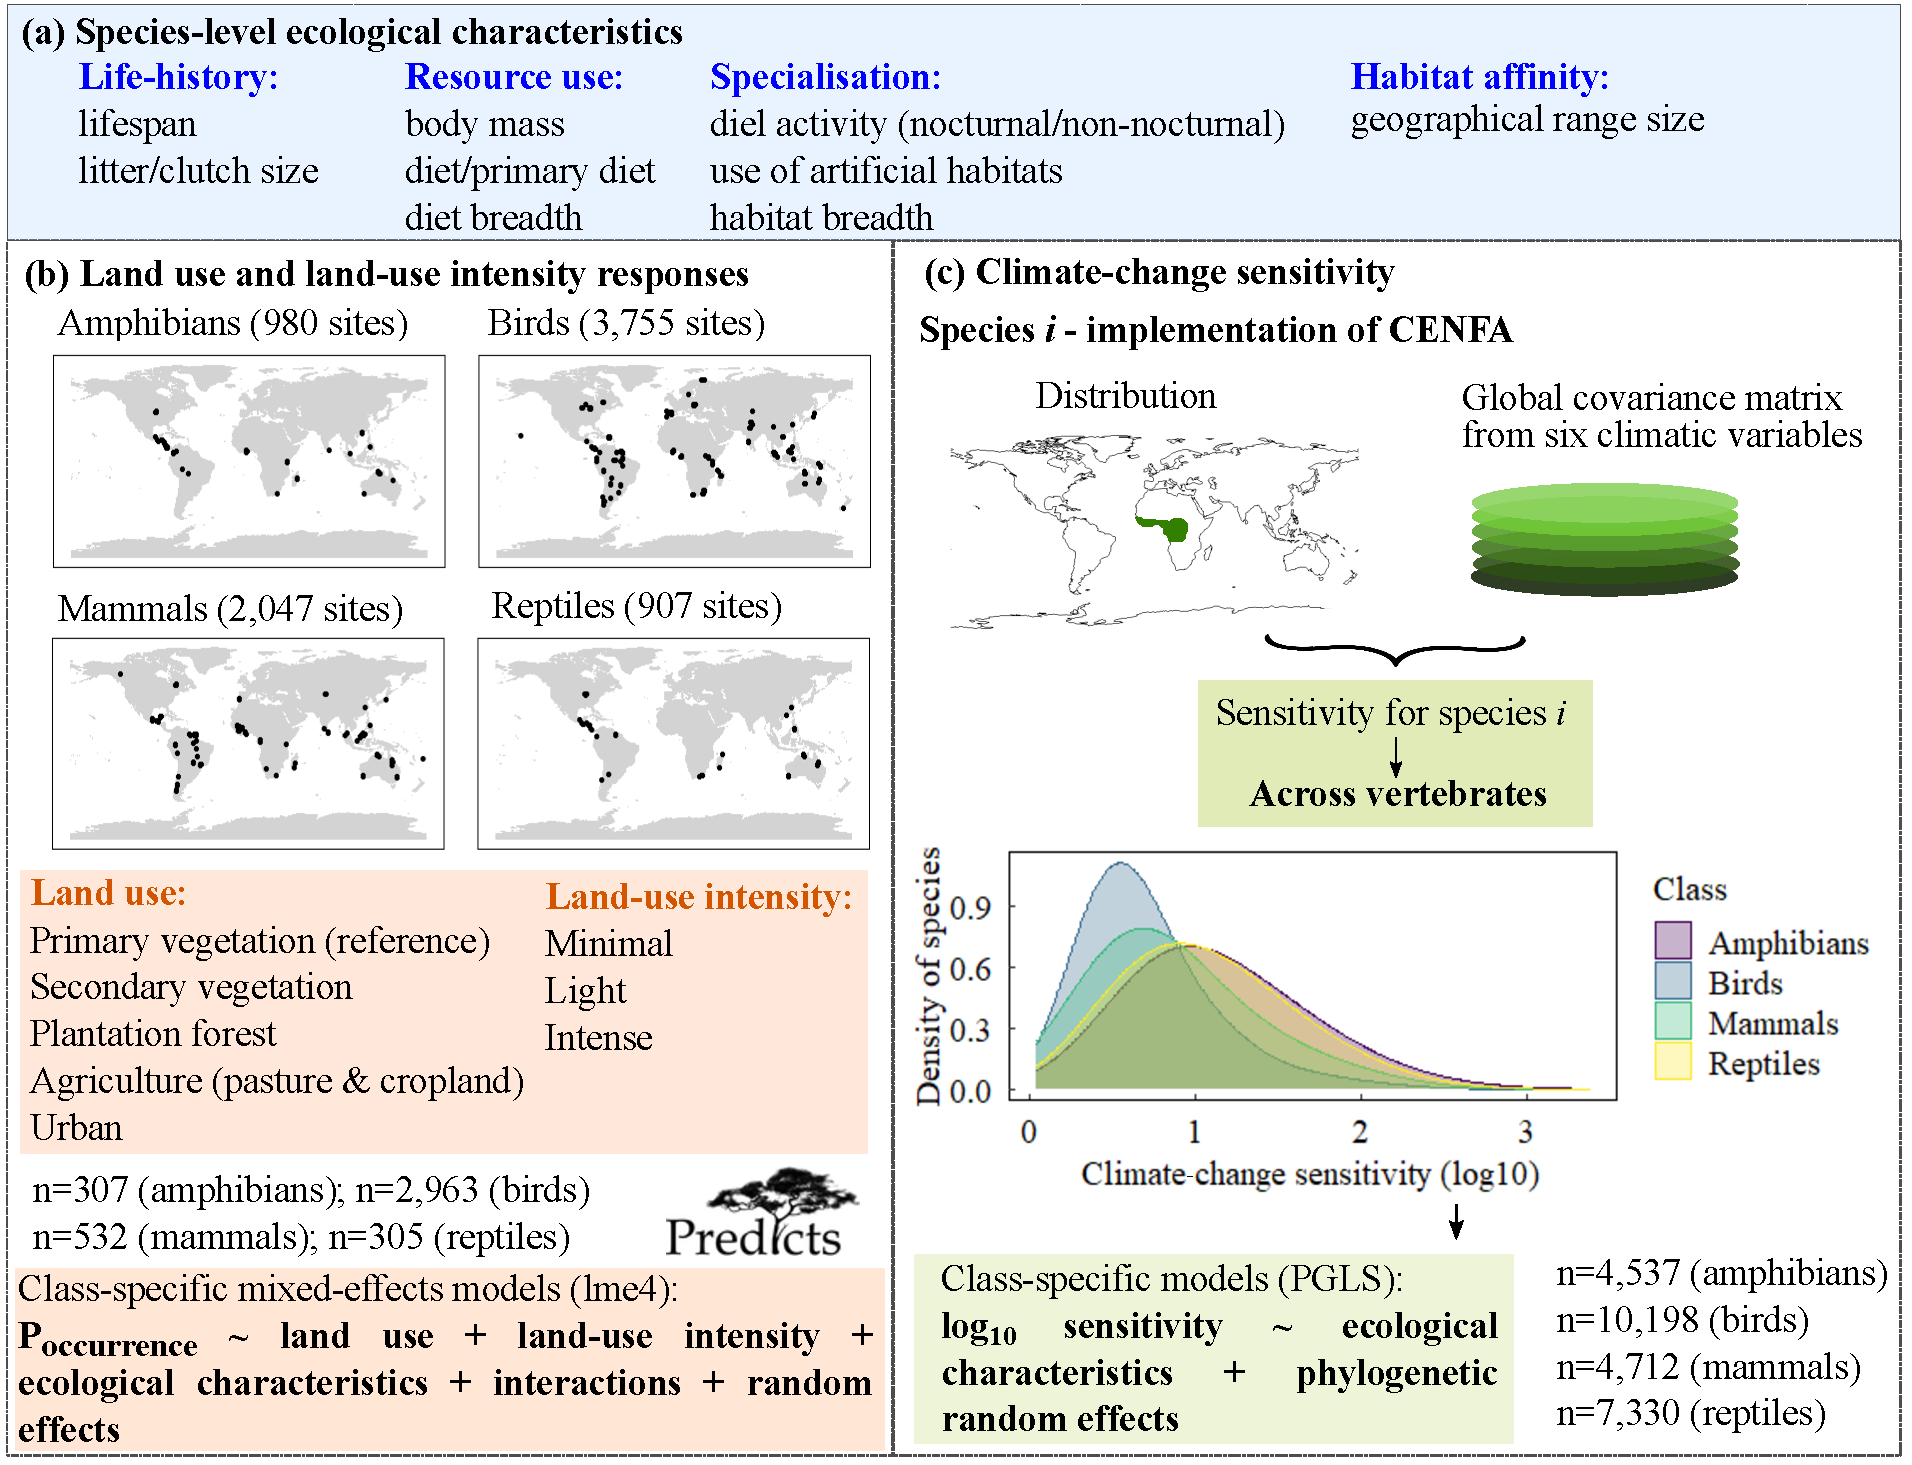
\includegraphics[scale=0.55]{figures/Chapter4/Figure1}
\caption[Framework of the study]{\textbf{Framework of the study.} \textbf{(a)} I collected ecological trait data and geographical range areas across terrestrial vertebrates (termed `ecological characteristics'). I then used two independent approaches to assess the influence of these characteristics on species' responses to land-use and on species' climate-change sensitivity. \textbf{(b)} To assess the influence of traits on responses to land use and land-use intensity in each vertebrate class, I combined the ecological characteristics with the PREDICTS database. \textbf{(c)} To estimate species sensitivity to climate change, I used the CENFA framework \citep{Rinnan2019}, which relies on the combination of species’ distributions with climatic variables to estimate sensitivity from properties of the species’ climatic niche space. I then built class-specific models to assess whether the ecological characteristics were associated with  species sensitivity to climate change.}
\label{chap4_fig1}
\end{figure}

\clearpage

\section{Methods}

\subsection{Ecological characteristics (Figure \ref{chap4_fig1}a)}

\subsubsection{Traits}

I obtained the six following traits from Chapter 2 (in which I presented a trait data compilation across terrestrial vertebrates): body size (body mass and/or length, depending on the class); a proxy for species lifespan (generation length for mammals and birds; age at sexual maturity for amphibians; and maximum longevity for reptiles); litter or clutch size; diel activity; habitat breadth; and use of artificial habitats. I chose these traits because 1) they were available across all vertebrate classes, at least for a subset of species, allowing for a comparative assessment; and 2) they relate to species life-history, ecology, and resource use, such that they might influence species' land-use responses and climatic niche properties (and thus expected climate-change sensitivity). I couldn't capture intraspecific variation in trait values, and instead I used single mean values for all traits.

I enhanced the trait data from Chapter 2 with species-level estimates of diet, lacking in the published database but likely important for understanding species sensitivity to human pressures. For birds and mammals, I collected estimates of species primary diet (i.e., the diet inferred from the combination of food items totalling more than 50\% of species’ consumption), from the EltonTraits database \citep{Wilman2014}. For amphibians and reptiles, obtaining species \textit{primary} diet was not possible, as there were no data available on the relative consumption of different food items. For amphibians, the AmphiBIO database \citep{Oliveira2017} provided information on species consumption of different food items (just in terms of presence/absence in the diet, but without estimation of their percent use), so I inferred diet on the basis of these reported food items (however the coverage was low, with more than 75\% of the species missing diet information; Appendix 3, Figure \ref{SI_4_fig1}). For reptiles, there was no available data collection describing diet. For both reptiles and amphibians, I supplemented the existing datasets by collecting data on species consumption from published sources  (recording the presence/absence of different food items in species consumption), for an additional 108 amphibians and for 239 reptiles (see Appendix 3, S4.1: `Compiling diet information'). 

I standardised the diet data across the vertebrate classes, by grouping species in five different diet categories: vertebrate eaters; invertebrate eaters; plant/seed eaters; fruit/nectar eaters; and omnivores  (for mammals and birds, species were classified as omnivores when all food items had a percent use $\leq$50\%; and for amphibians and reptiles, when species where known to consume both plant and animal matter). I also calculated species diet breadth -- the total number of recorded food items (in terms of presence/absence) known to be consumed by a species. More information on the compilation of dietary information can be found in Appendix 3, S4.1: `Compiling diet information'. 

\subsubsection{Geographical range area}
I used extent-of-occurrence maps from BirdLife International for birds (\url{http://datazone.birdlife.org/species/requestdis}), from the IUCN Red List for mammals and amphibians \citep{IUCN2020}, and from \citet{Roll2017} for reptiles (all downloaded in April 2020). I excluded areas occupied during non-breeding seasons and areas falling outside species known elevational limits (following Chapter 2). The range maps were then converted to the raster format (`raster' package, version 3.5.15 \citet{rasterpackage}), and I estimated species geographical range areas using a resolution of 1 km$^2$ with Behrmann's equal-area projection.  Although range area cannot be considered a trait (which is a property measurable at the level of individual organisms), I included range area in the analyses because past work has shown that range area is an important correlate of species' responses to land use \citep{Newbold2018a} and climate change \citep{Thuiller2005}. In addition, range area may correlate with other aspects of species' ecology that I could not include directly in the analysis because of limited data availability, such as dispersal ability \citep{Capurucho2020}.

\subsubsection{Phylogenies}
I used information on species' phylogenetic position in the imputations of missing trait values (see next section), and also to control for phylogenetic relationships in the models investigating effects of ecological characteristics on species' estimated climate-change sensitivity. Class-specific phylogenetic trees were downloaded April 2020 from \url{https://zenodo.org/record/3690867#.Xyc5wyhKhPZ} for mammals (Phylacine 1.2; \citet{Faurby2018, Faurby2020}); and from \url{https://data.vertlife.org/} for amphibians \citep{Jetz2018}, birds \citep{Jetz2012} and squamates \citep{Tonini2016}. For each class, I used a consensus tree obtained with the TreeAnnotator programme of the BEAST software (Bouckaert et al. 2014), from an available distribution of 1000 trees. 

\subsection{Imputations of missing trait values}
For some of the traits and classes, there was a substantial proportion of missing trait values (Figure \ref{SI_4_fig1}). To fill these gaps, I imputed missing trait values using random forests, implemented with the `missforest’ function of the `missForest’ package in R (version 1.4, \citet{Stekhoven2012, Stekhoven2016}). `missforest' is one of the best methods for missing-value imputations when working with continuous and categorical variables, and when including species phylogenetic position as a predictor \citep{Penone2014, Debastiani2021}. After showing that several traits were strongly phylogenetically conserved (Table \ref{SI_4_Table1}), I included ten phylogenetic eigenvectors in the imputations \citep{Penone2014}, as well as taxonomic orders as a categorical variable (included to account for the taxonomic positions of species that were not represented in the phylogenies). Full details are given in Appendix 3 (S4.2: `Imputing missing trait values'). After imputation, continuous traits were log$_{10}$-transformed to improve normality (except for habitat and diet breadth, which I square-root transformed; this transformation was more appropriate here because the distributions of habitat breadth and diet breadth tended to be less right-skewed than that of the other traits, and the range of values was smaller).

\subsection{Characterizing the influence of traits on species' land-use responses (Figure \ref{chap4_fig1}b)}

\subsubsection{Vertebrate assemblage composition}

To compare vertebrate assemblages in different land-use types, I used the PREDICTS database \citep{Hudson2014, Hudson2017}. PREDICTS is a collection of independent studies that have sampled biodiversity in sites of varying land use and land-use intensity. Samples are mostly of species abundance, sometimes species occurrence, and rarely just overall species richness. It is one of the most comprehensive such databases to date, with 4,107 vertebrate species sampled across 7,689 sites considered in this work (Figure \ref{chap4_fig1}b). In PREDICTS, sites are assigned to one of the following land-use categories: primary vegetation (native vegetation); secondary vegetation, plantation forest, pasture, cropland, and urban (disturbed land uses; see Table \ref{SI_4_Table2} and \citet{Hudson2014, Hudson2017} for more details). Each site is also characterised in terms of land-use intensity based on land-use-specific criteria (such as mechanisation degree, crop diversity and agricultural inputs for cropland; \citet{Hudson2014}). Land-use intensity is divided into three categories to reflect the degree of human transformation and impacts on the land: minimal, light or intense. Here, I considered minimally-used primary vegetation to be the least-disturbed reference land use against which I compare all other land-use types. I grouped pasture and cropland together into a category I termed `agricultural'. As the design of the PREDICTS database is not balanced, sample sizes varied among classes and land-use types (Figure \ref{SI_4_Figure4}).

\subsubsection{Full models (all-predictor models)}

Within each vertebrate class, I investigated whether interactions among the ecological characteristics, land use and land-use intensity explained species occurrence probability. I fitted four binomial mixed-effects models (one for each class), using the `lme4' package (version 1.1-23; \citet{Bates2015}), with random effects accounting for study, site and species identity to account for the nested design of the database, taxonomic non-independence, and repeated observations among species. I did not consider interactions among the ecological characteristics, but I included interactions between land use and ecological characteristics, and between land-use intensity and ecological characteristics. Before fitting the models, I checked the degree of multicollinearity among explanatory variables using generalised variance inflation factors (GVIF; \citet{Fox1992}), with a threshold of 5 for the detection of multicollinearity (Tables \ref{SI_4_Table3}-\ref{SI_4_Table8}). For amphibians and reptiles, including both diet and diet breadth was problematic, so I excluded diet from the set of predictors for these classes on the basis of the GVIF scores . Models investigating the effects of diet were built separately (see next section, `Partial models').

I did not use phylogenetic random effects directly in the models because of the computational load required by such models when working with several hundred or thousands of species. However, I checked the phylogenetic signal in the models' residuals using Pagel’s $\lambda$ \citep{Pagel1999}. Thus, in each class, the model fitted was:\\
\\
$\text{P\textsubscript{occurrence}}\sim \text{land use} + \text{land-use intensity} + \text{species-level ecological characteristics} + \\
\text{land use}:\text{species-level ecological characteristics} + \\
\text{land-use intensity}:\text{species-level ecological characteristics} + \\
(1|\text{sudy identity}) + (1|\text{site identity}) + (1|\text{species identity})$.\\

To verify that the models' estimates were robust to any violation of distributional assumptions, I fitted the models again using a Bayesian framework (using the `MCMCglmm' package version 2.32, \citet{mcmcglmm}).

\subsubsection{Partial models (single-predictor models)}
In addition to the full models, I fitted partial models for each class. These were fitted to visualise occurrence patterns for each trait independently of other traits. The structure of the models was similar to that of the full models, except that I included a single species-level characteristic at a time in each model. 

\subsubsection{Effects of categorical ecological characteristics on species' occurrence probability (Figure \ref{chap4_fig2}a)}
The influence of categorical traits on species' responses to land use and land-use intensity can be visualised in two ways: either by comparing occurrence probability in different land-use types relative to species with similar traits (I term such effects `among land-use type effects', Figure \ref{chap4_fig2}a); or by comparing occurrence probability in a given land-use type relative to species with different traits (I term such effects `within land-use type effects', Figure \ref{chap4_fig2}a). 

\begin{itemize}
\item
Within land-use type effects (Figure \ref{chap4_fig2}a): from the full, all-predictor models fitted for each class, I focused on the interactive effects between land use and ecological characteristics (and between land-use intensity and ecological characteristics). These interactions indicated whether, in a given land-use type, there were any significant differences in occurrence probability between species with different traits. In other words, I looked at whether any trait level lowered or increased occurrence probability in each land-use type, compared to a reference trait level. I used this approach for all the categorical predictors, except diet (interpreting within land-use type effects for primary diet being complicated by the fact that there were more than two levels for this trait).  
\item
Among land-use type effects (Figure \ref{chap4_fig2}a): from a partial model, I predicted occurrence probability in the different land uses for all different levels of the trait. The partial models allowed to visualise occurrence patterns across land-use types for single explanatory variables, without having to account for the values of other variables. I used this approach to evaluate the influence of diet on species' land-use responses.
\end{itemize}


\subsubsection{Effects of continuous ecological characteristics on species’ occurrence probability (Figure \ref{chap4_fig2}b)}
For a given continuous ecological characteristic, any effect of land use or land-use intensity can be assessed through changes in the slope of the relationship between the ecological characteristic and occurrence probability (Figure \ref{chap4_fig2}b). When an ecological characteristic negatively impacts occurrence probability in a disturbed land use, I expect the slope of the relationship to be more negative than the slope for the reference land use (minimally-used primary vegetation). Focussing on slopes does not allow to infer absolute changes in occurrence probability across land-use types (e.g., a positive slope in a disturbed land use does not mean that there are absolute increases in occurrence probability in that land use, but only that higher values of the ecological characteristic are associated with relatively higher occurrence probability in that land-use type). This is because I do not assess changes in the mean occurrence probability here (which would require to consider the intercept of the relationship between the ecological characteristic and occurrence probability in different land-use types). Thus, I only capture `within land-use type' effects for continuous predictors.

\vspace{0.5cm}
%% Figure 2 = assessing effects 
\begin{figure}[h!]
\centering
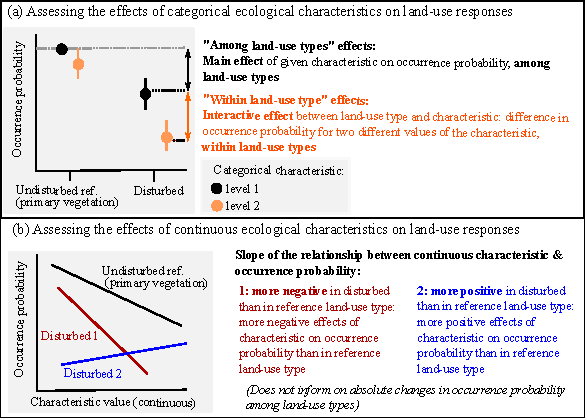
\includegraphics[scale=1.6]{figures/Chapter4/Figure2}
\caption[Assessing the effects of ecological characteristics on species' land-use responses: methodology for (a) categorical characteristics and (b) continuous characteristics.]{\textbf{Assessing the effects of ecological characteristics on species' land-use responses: methodology for (a) categorical characteristics and (b) continuous characteristics.} \textbf{(a)} For all categorical characteristics, except diet, I look at `within land-use type' effects, asking whether there are significant differences in occurrence probability among species with different ecological characteristics in a given land-use type. For diet, I look at `among land-use type' effects, comparing species occurrence probability in disturbed land uses versus that in primary vegetation  (I chose this approach here because visualising `within land-use type' effects for diet is complicated by the fact that there were more than two levels for this categorical trait). \textbf{(b)} For continuous characteristics, I focus on the relationship with occurrence probability, and I investigate how the slope of this relationship is affected by land-use type, i.e. a `within land-use type' effect.}
\label{chap4_fig2}
\end{figure}

\subsubsection{Validation on complete trait data subset (no imputed trait values)}
To assess whether the results were robust to trait imputation uncertainty, I fitted the models again for the subset of species for which I had complete, non-imputed data for all ecological characteristics. The models' structure was unchanged for birds and mammals. For amphibians, I excluded both diet and litter/clutch size because of multicollinearity issues, and I also excluded lifespan proxy and body mass (as there were too many missing values in the dataset, 85\% and 59\% respectively). For reptiles, I excluded both diet and body mass because of multicollinearity issues.

\pagebreak

\subsection{Characterizing the influence of traits on species' sensitivity to climate change (Figure \ref{chap4_fig1}c)}

I estimated climate-change sensitivity across vertebrate species using the `Climate-niche Factor Analysis' (CENFA) approach developed by \citet{Rinnan2019}, implemented with the `CENFA'  R package  version 1.1.1 \citep{CENFA}. CENFA is a spatial approach for estimating species' climate-change sensitivity, exposure, and vulnerability. CENFA combines distribution data with climatic variables to estimate sensitivity and vulnerability from properties of species' climatic niches (see \citet{Rinnan2019} for details). CENFA has been used in previous studies focused on a small number of species or on a few taxonomic groups, but to my knowledge has not yet been applied across all terrestrial vertebrates.

\subsubsection{Historical climate data}
I used global climate data  from WorldClim version 2.1 \citep{Fick2017}. I downloaded 19 climatic variables at a resolution of 2.5 arcminutes ($\sim$4.6 km$^2$ at the Equator). I removed variables that were strongly collinear with any other climatic variables (using a threshold of 0.65 for Spearman correlation coefficients). I obtained six groups of intercorrelated variables (using the `removeCollinearity' function from the `virtualspecies' R package version 1.5.1 \citep{virtualspecies}; Figure \ref{SI_4_Figure5}), and randomly selected one climatic variable in each group. The final set comprised six climatic variables: annual mean temperature (bio1), mean diurnal temperature range (bio2), maximum temperature of the warmest month (bio5), annual precipitation (bio12), precipitation seasonality (bio15), and precipitation of the coldest quarter (bio19).

\subsubsection{Estimating climate-change sensitivity from CENFA}
All climatic variables and distribution files were re-projected to a resolution of 5 km$^2$ in the Behrmann equal-area projection. I picked this resolution because the coarser the resolution, the more climate-change sensitivity tended to be underestimated for narrowly distributed species (Figures \ref{SI_4_Figure6} \& \ref{SI_4_Figure7}). However, finer resolutions demand a large amount of memory space when working at global scales across all terrestrial vertebrates. I found the 5-km$^2$ resolution to be an acceptable trade-off between computational load and accuracy of the sensitivity estimations. However, when working at 5-km$^2$ resolution, there were still some narrowly distributed species for which sensitivity was likely underestimated (Figure \ref{SI_4_Figure7}). Thus, I chose to exclude species with a range area $\leq$ 100 km$^2$ from further analyses (i.e., excluding narrow-ranging species whose distributions could intersect up to 4 grid cells). In doing so, the sample size was reduced by 660 species for amphibians, by 142 species for birds, by 129 species for mammals, and by 615 species for reptiles (the final sample sizes were: n=4,537 for amphibians; n=10,198 for birds; n=4,721 for mammals; n=7,330 for reptiles). My results were overall robust to the exclusion of these species (see Results section). 

I then combined the climate data with the species' distributions to estimate sensitivity to climate change, applying the CENFA framework across terrestrial vertebrates (Figure \ref{chap4_fig1}c). Further details of the implementation of the CENFA framework are given in Appendix 3 (S4.5: `Implementing Climate-niche Factor Analysis across terrestrial vertebrates').


\subsubsection{Climate-change sensitivity models}
I used phylogenetic least-square (PGLS) regressions, implemented in the `caper' R package version 1.0.1 \citep{caper}, to assess the effects of ecological characteristics on species estimated sensitivity to climate change, while controlling for phylogenetic relationships among species. I combined the ecological characteristics and the phylogenies using the `comparative.data' function from the `caper' package, and then built class-specific models to explain climate-change sensitivity with the ecological characteristics (Figure \ref{chap4_fig1}c). Before fitting the models, I checked for multicollinearity among the predictors using GVIF scores. Across all classes, the models included all the main effects of the ecological characteristics, except for amphibians, for which I dropped diet breadth (which was strongly collinear with diet; Tables \ref{SI_4_Table9}-\ref{SI_4_Table13}). For the continuous predictors, I fitted third-order polynomials to allow for non-linearity of the responses (I included third order polynomials for the climate-change sensitivity models but not for the land-use models because the PGLS model had a simpler structure than the land-use models, were less computationally intensive, and also because the number of estimated parameters was already high for the land-use models without allowing for third-order polynomials). As such, the general form of the PGLS models was: \\
\vspace{0.3cm}
$\log_{10}\text{(climate-change sensitivity)}  \sim  \text{poly(log\textsubscript{10}(continuous ecological characteristics),3)} +\\
\text{categorical ecological characteristics} + 
\text{phylogenetic random effects}$.


\subsubsection{Models' robustness}
To check whether the results were robust to the exclusion of species whose range area was $\leq$100 km$^2$, I repeated the models on all species (including those with range area $\leq$100 km$^2$: n=5,208 for amphibians; n=10,340 for birds; n=4,844 for mammals; n=7,951 for reptiles). 

Finally, to assess the degree to which the results were robust to trait imputation uncertainty, I fitted the models again for the subset of species for which I had empirical (i.e., non-imputed) trait estimates. Diet was excluded for amphibians and reptiles on the basis of high collinearity (GVIF$>$5). I fitted first-order polynomials here because of the substantially reduced sample size compared to the main models.




\section{Results}

\subsection{Land-use responses}

\subsubsection{`Within land-use type' effects (Table \ref{chap4_table1}a)}
Land-use, land-use intensity, species' ecological characteristics and their interactions had significant effects on species occurrence probability. Significant interactive effects between land use and ecological characteristics (and between land-use intensity and ecological characteristics) reflected differences in the ability of species with different ecological characteristics to cope within the disturbed land-use types (Table \ref{chap4_table1}a). Across all classes, species with narrower geographical range areas, smaller habitat breadth and inability to exploit artificial habitats showed greater decreases in occurrence probability within disturbed land uses, than species with larger range areas, larger habitat breadth and ability to exploit artificial habitats (the only exceptions were opposite effects found for mammals and reptiles for habitat breadth in two of the land-use types). The effects of the other ecological characteristics differed in direction depending on class and land use, impeding any generalisation (Table \ref{chap4_table1}a). For instance, I found that being smaller and longer-lived was associated with decreases in occurrence probability for birds found in agricultural areas, but with increases in occurrence probability for urban birds; and that  longer-lived species tended to be more negatively affected for mammals and reptiles, whereas I found evidence of opposite trends for amphibians.

I would like to highlight that the `within land-use type' effects summarised in Table \ref{chap4_table1}a do not necessarily reflect occurrence patterns among land-use types. For example, in all classes, `among land-use type' effects derived from partial models showed that occurrence probability in disturbed land uses was strongly negatively affected for natural habitat specialists, compared with primary vegetation levels Figure \ref{SI_4_Figure10}. On the other hand, in most classes and disturbed land uses, artificial habitat users either increased or showed no significant difference in occurrence probability. One exception was for reptiles, where the effect of habitat specialisation was mostly non-significant within land-use types (Table \ref{chap4_table1}a), with both natural habitat specialists and artificial habitat users showing important declines in some disturbed land uses (e.g., intensely-used agricultural areas, Figure \ref{SI_4_Figure10}d). Similarly, the occurrence probability of both nocturnal and non-nocturnal species was negatively impacted in disturbed land uses compared with primary vegetation (Figure \ref{SI_4_Figure11}), such that land-use responses were not distinguishable between nocturnal and non-nocturnal species for all classes and land-use types. 


%% Synthesis table 
\begin{landscape}
\begin{table}
\centering
\caption[Summary of the effects of the ecological characteristics (except for primary diet) on species' responses to disturbed land uses (`within land-use type' effects) and on species' climate-change sensitivity, for each Class of terrestrial vertebrates.]{\textbf{Summary of the effects of the ecological characteristics (except for primary diet) on (a) species' responses to disturbed land uses (`within land-use type' effects) and on (b) species' climate-change sensitivity, for each class of terrestrial vertebrates.} The symbol \colorbox{Salmon}{\textcolor{BrickRed}{\textbf{--}}} indicates where a characteristic has a significant negative effect on occurrence probability within a disturbed land-use type (within any of the land-use intensities), or where the characteristic renders species significantly more sensitive to climate change. A \colorbox{YellowGreen}{\textcolor{ForestGreen}{\textbf{+}}} indicates a significantly  positive effect of a characteristic on occurrence probability in a land-use type (within any of the land-use intensities), or significantly lower sensitivity to climate change. For the land-use effects, I report `within land-use type effects' here, that is, within a disturbed land use whether there were significant differences in occurrence probability among species with different trait values (see Figure \ref{chap4_fig2}). These effects were derived from the interactive terms of the full, all-predictor models.}
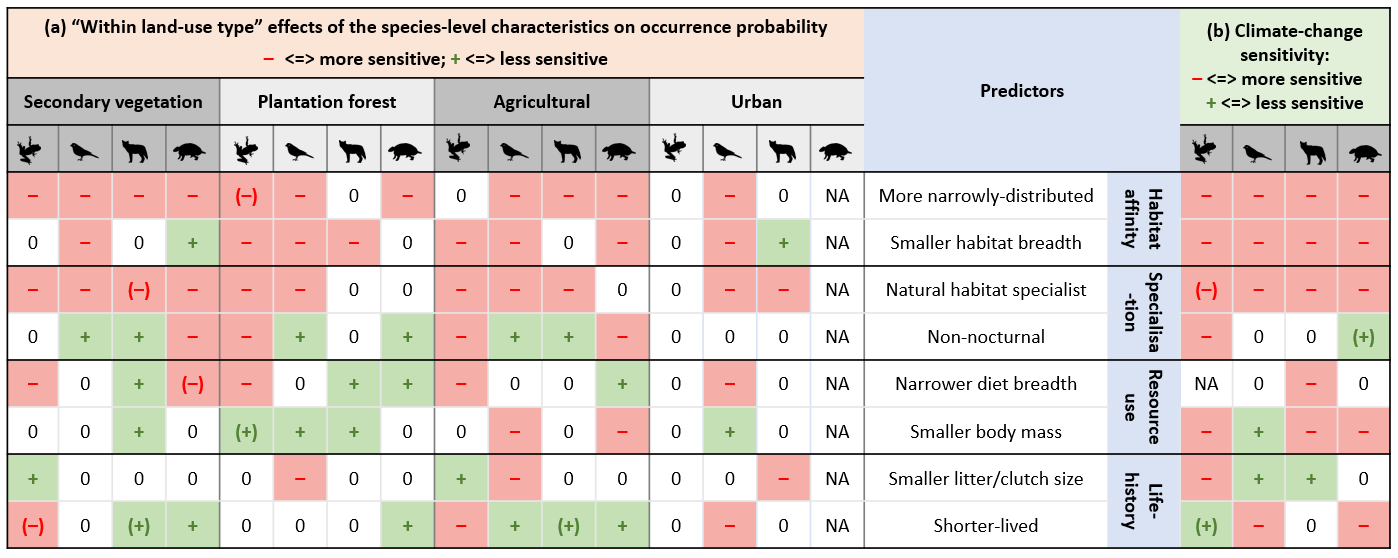
\includegraphics[scale=0.8]{figures/Chapter4/Synthesis_table}
\label{chap4_table1}
\end{table}
\end{landscape}

\subsubsection{Effects of diet on species' occurrence probability (Figure \ref{chap4_fig3})}
In all classes, diet had significant effects on occurrence probability in disturbed land uses (Figure \ref{chap4_fig3}). Changes in occurrence probability in disturbed land uses differed among classes and dietary groups. Overall, invertebrate eaters tended to be negatively affected in disturbed land uses (e.g., -66\% average declines in occurrence probability for amphibians in intensely used agricultural areas, compared with minimally-used primary vegetation). Omnivores were both negatively and positively impacted, showing both important decreases (e.g., -81\% for reptiles in intensely used plantation forest) as well as strong increases (e.g., +43\% for lightly used urban areas in birds). Overall, fruit/nectar eaters showed important declines in occurrence probability for mammals and birds, as opposed to plants/seeds eaters, whose occurrence probability tended to be strongly positively affected for birds, and dependent on land-use intensity for mammals (with increases in minimally-used land-types, but not in more intensely-used land-types). Finally, I also detected significant changes in occurrence probability for vertebrate eaters, with some declines for mammals in agricultural areas (-75\% on average in intense uses), but also some increases (e.g., +43\% on average for birds in lightly used agricultural areas).


\subsubsection{Explanatory power for the full models \& variance explained by each characteristic (Figure \ref{chap4_fig4})}
Overall, land use, land-use intensity and the ecological characteristics explained a small amount of the total variation in species' occurrence probability (marginal R$^2$: 0.15 for amphibians; 0.054 for birds; 0.15 for mammals; 0.13 for reptiles), in part because the random effects explained a substantial proportion (conditional R$^2$: 0.59 for amphibians; 0.61 for birds; 0.72 for mammals; 0.57 for reptiles). The relative importance of traits explaining the most variation differed among classes, with interactions between land use and habitat breadth explaining the most variation in amphibians and birds, but interactions between land use and body mass explaining the most variation for mammals, and interactions between land use and lifespan explaining the most variation for reptiles (Figure \ref{chap4_fig4}a). 

Finally, the models' diagnostics showed evidence of deviations from distributional assumptions (diagnostic plots for the full models are shown in Figures \ref{SI_4_Figure12}-\ref{SI_4_Figure15}). However, when estimated from a Bayesian framework, the models’ estimates were mostly congruent (results not shown), so the frequentist approach I used with `lme4' was robust despite the deviations from distributional assumptions. The phylogenetic signals in the models' residuals were low and not significant (Pagel’s $\lambda$ $<$ 0.01 for amphibians and reptiles, p $\approx$ 1; $\lambda$  = 0.13 for mammals, p = 0.09; $\lambda$  = 0.01 for birds, p = 0.56), despite not having included phylogenetic random effects.

\pagebreak
%% Diet figure
\begin{figure}[h!]
\centering
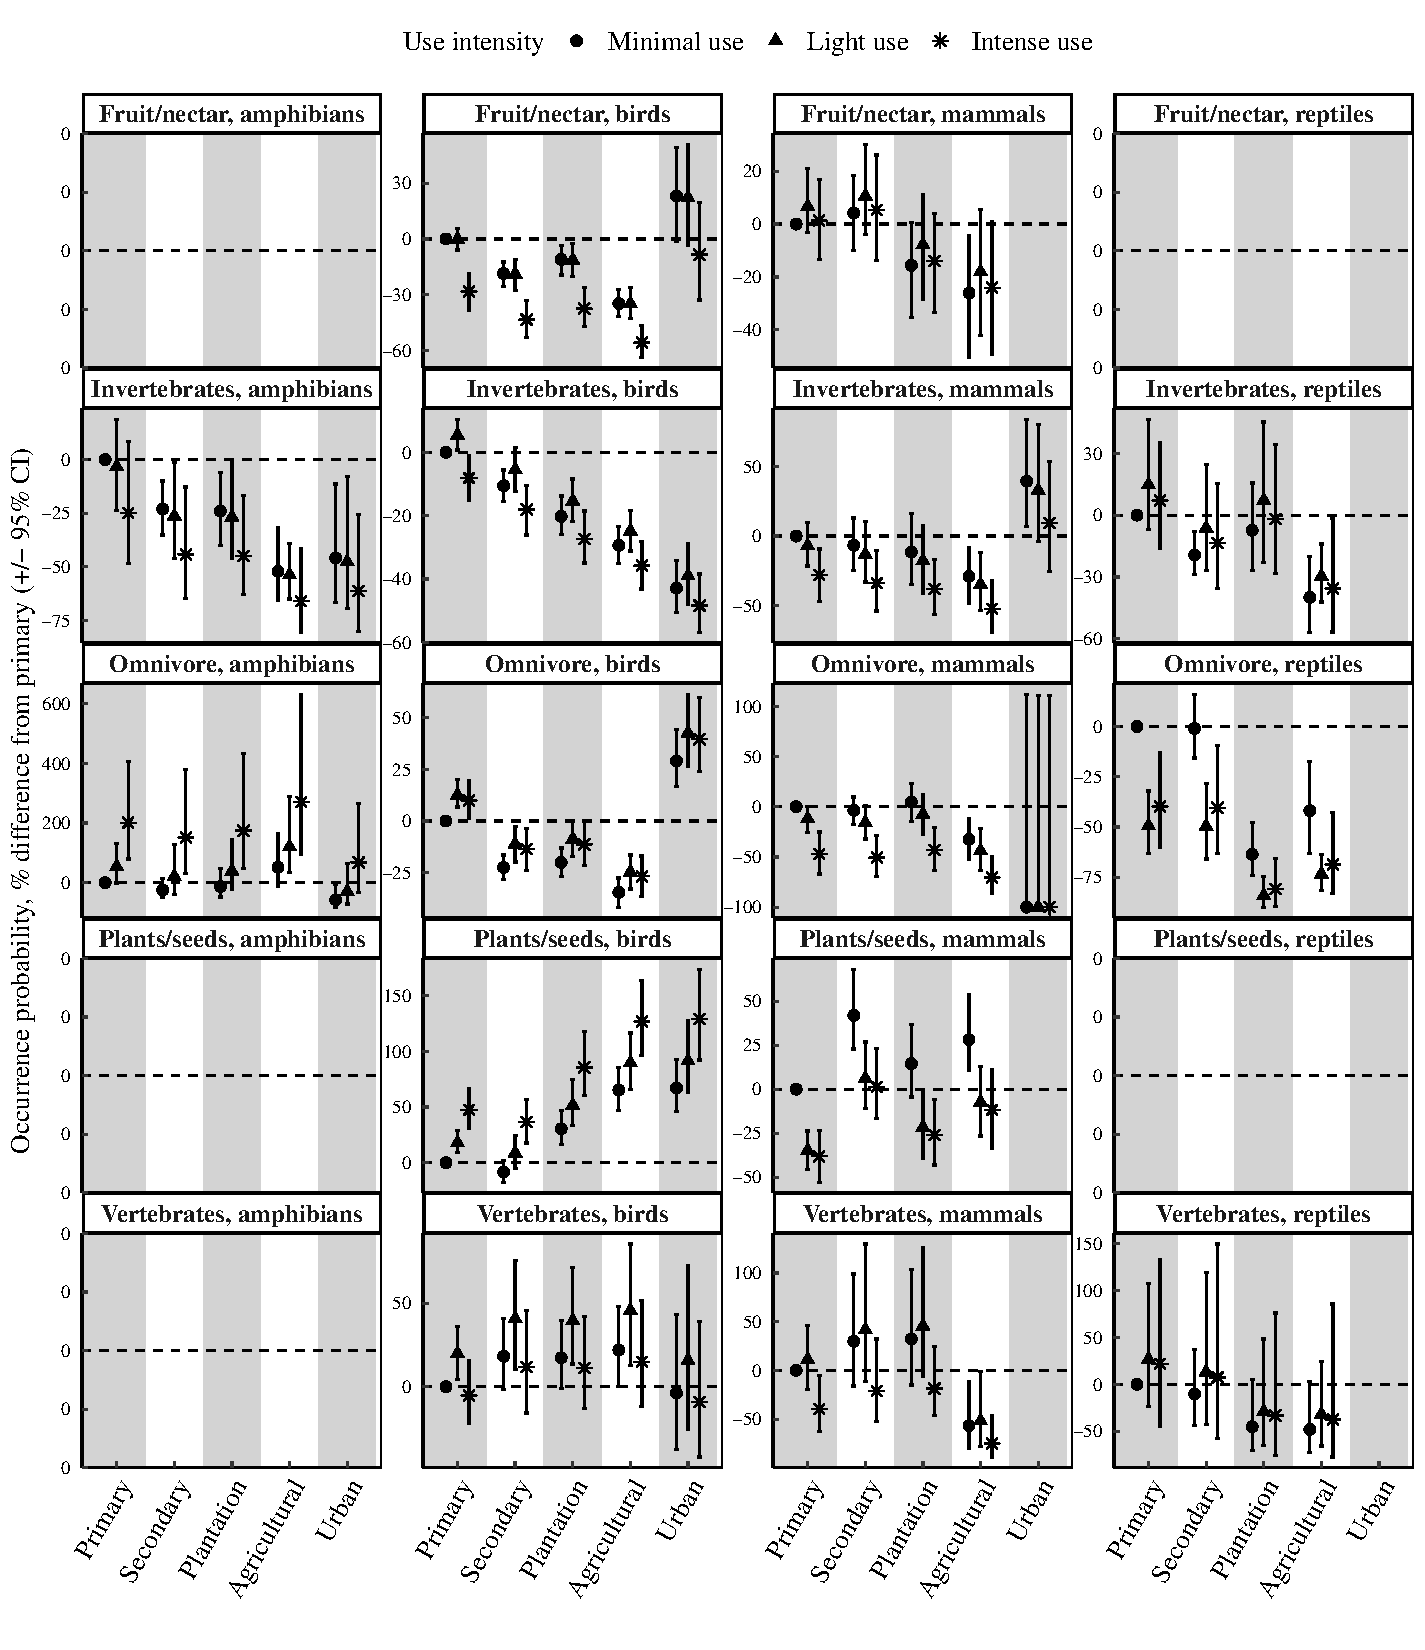
\includegraphics[scale=0.7]{figures/Chapter4/Figure3_V2}
\caption[Predicted occurrence probability as a function of land use, land-use intensity, diet and their interactions, for each class of terrestrial vertebrates.]{\textbf{Predicted occurrence probability as a function of land use, land-use intensity, diet and their interactions, for each class of terrestrial vertebrates} (median $\pm$ 95\% confidence interval; the predictions are rescaled with reference to minimally-used primary vegetation). The predictions were obtained from the partial models fitted for each class, considering only diet among the ecological characteristics. Empty plots are drawn where there were no data for a diet category for a given class. Effects could not be estimated for urban reptiles, as well as for urban vertebrate, fruit/nectar and plant/seed eaters for mammals because there were no sampled species. Primary: primary vegetation; Secondary: secondary vegetation; Plantation: plantation forest; Agricultural: cropland and pasture.}
\label{chap4_fig3}
\end{figure}


\pagebreak
%% Figure Variance
\begin{figure}[h!]
\centering
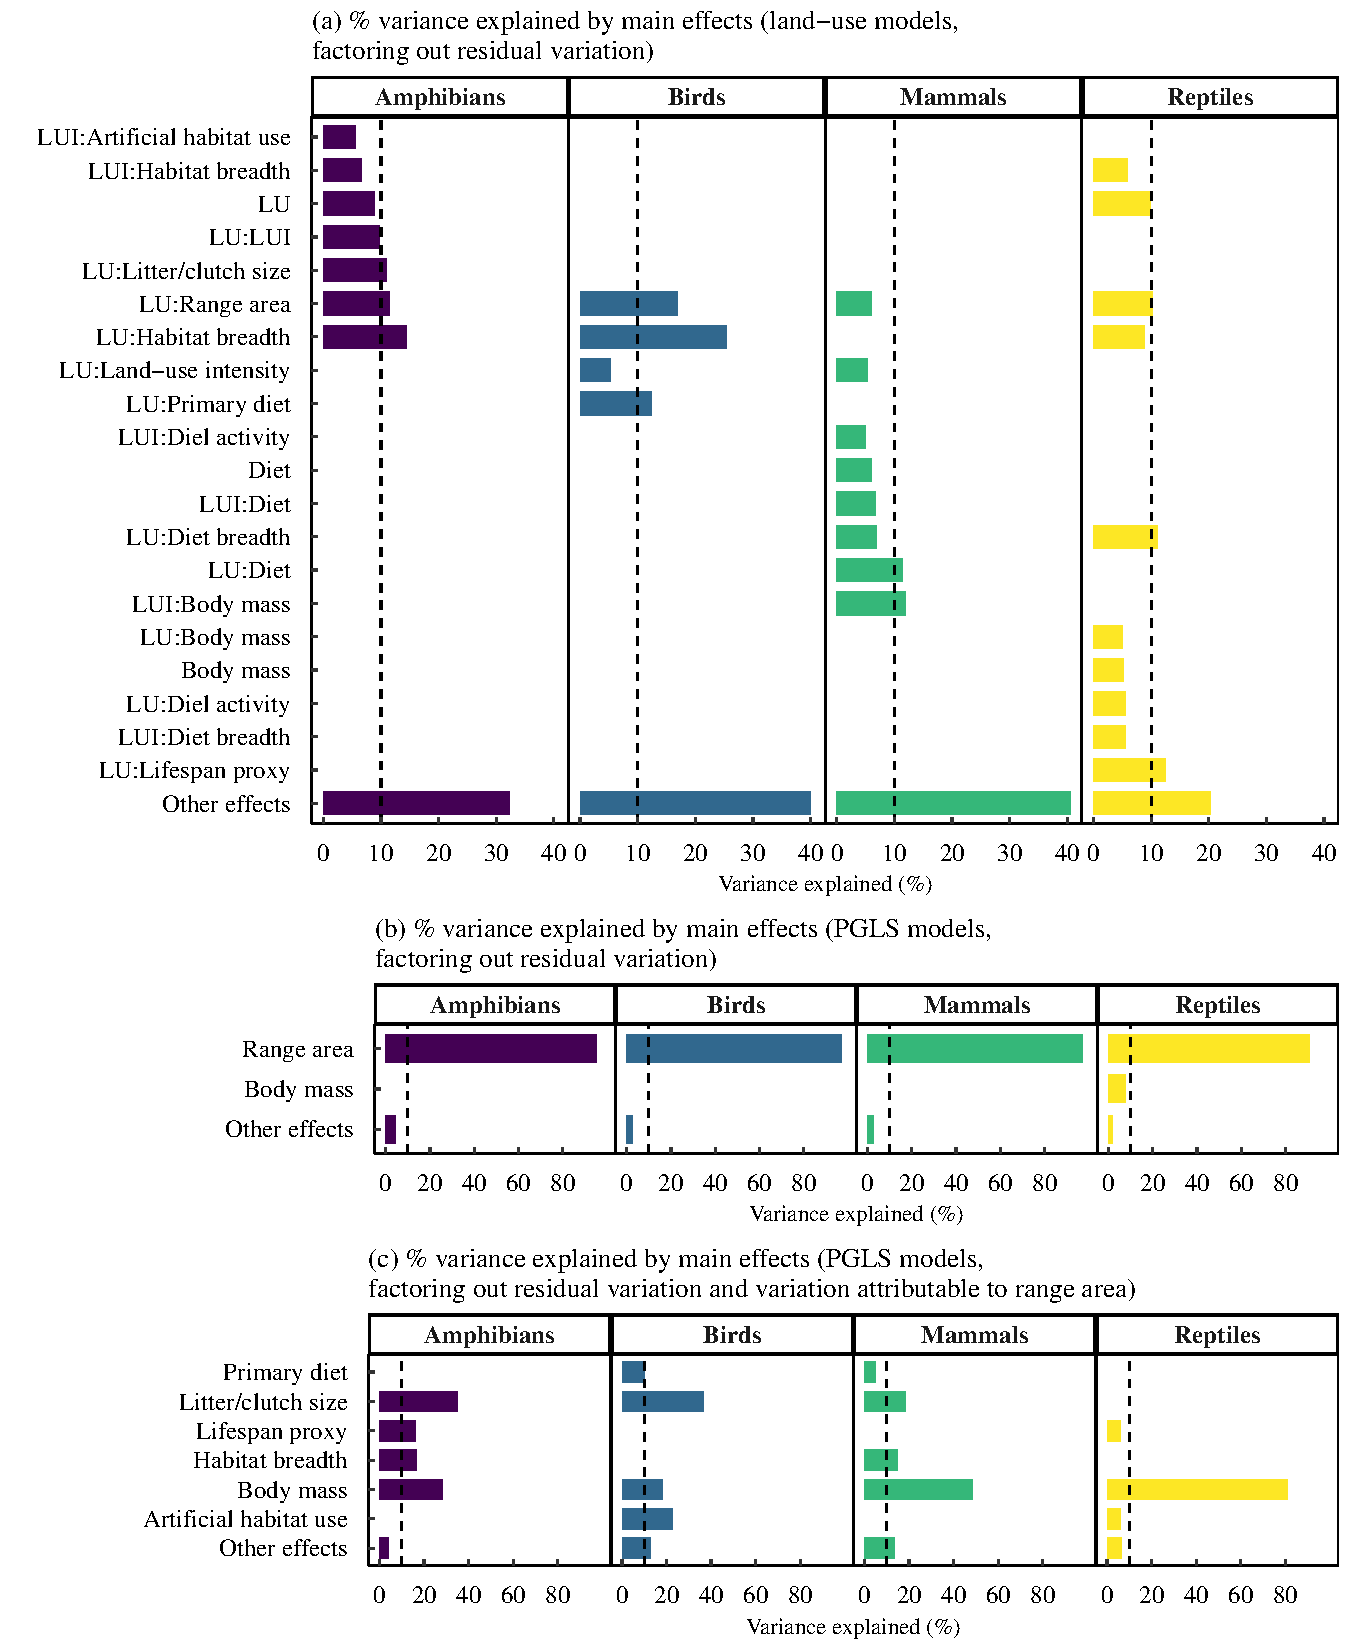
\includegraphics[scale=0.7]{figures/Chapter4/Variance_breakdown.pdf}
\caption[Proportion of the explained variance attributable to each of the main effects in the land-use and climate-change sensitivity models]{\textbf{Proportion of the explained variance attributable to each of the main effects for (a)} the mixed-effects models fitting the effects of land use, land-use intensity, and ecological characteristics on species occurrence probability (after factoring out residual variation); \textbf{(b)} for the phylogenetic least-squares regressions investigating whether the ecological characteristics explained climate-change sensitivity (after factoring out residual variation); and \textbf{(c)} for the phylogenetic least-squares regressions investigating whether the ecological characteristics explained climate-change sensitivity (after factoring out the variance explained by geographical range area and the residual variation). The dashed vertical lines mark 10\% explained variance (for visualisation purposes). I individually show all the effects that explain more than 5\% of the overall variation. Effects that individually explain less than 5\% of the overall variation are grouped together as `Other effects'. LU: land use; LUI: land-use intensity.}
\label{chap4_fig4}
\end{figure}

\clearpage
\pagebreak
\subsection{Climate-change sensitivity}
The ecological characteristics were significantly associated with climate-change sensitivity in all classes (Tables \ref{chap4_table1}b \& \ref{chap4_table2}, Figures \ref{chap4_fig5} \& \ref{chap4_fig6}); models' coefficients shown in Tables \ref{SI_4_Table14}-\ref{SI_4_Table17}). Overall, climate-change sensitivity was highest for amphibians (median log$_{10}$-sensitivity: 1.1; 95\% interpercentile range: 0.40-2.2), then reptiles (median log$_{10}$-sensitivity: 1.0; 95\% interpercentile range: 0.32-2.1), then mammals (median log$_{10}$-sensitivity: 0.76; 95\% interpercentile range: 0.22-2.0) and birds (median log$_{10}$-sensitivity: 0.62; 95\% interpercentile range: 0.21-1.77). In all classes, narrower geographical range area, smaller habitat breadth and being specialised on natural habitats were consistently associated with higher climate-change sensitivity (Table \ref{chap4_table1}b). However, other characteristics did not have consistent associations with climate-change sensitivity across classes, in different cases varying in both significance and direction. For instance, I found opposite associations between body mass and climate-change sensitivity for mammals, amphibians and reptiles on the one hand, and birds on the other hand. 


The PGLS models explained an important proportion of the overall variation in estimated climate-change sensitivity (adjusted R$^2$ = 0.64 for amphibians; 0.62 for birds; 0.63 for mammals and reptiles). Geographical range area explained the majority of this variation in climate-change sensitivity (about 60\% in all classes; Figure \ref{chap4_fig4}b), which largely reflects the design of the CENFA approach. When factoring out residual variation and variation explained by geographical range area, the relative importance of the traits as correlates of climate-change sensitivity varied among classes (Figure \ref{chap4_fig4}c), with body mass explaining the most variation for mammals and reptiles, and litter/clutch size explaining the most variation for amphibians and birds.

%% Figure climate-change sensitivity - categorical predictors
\begin{figure}[h!]
\centering
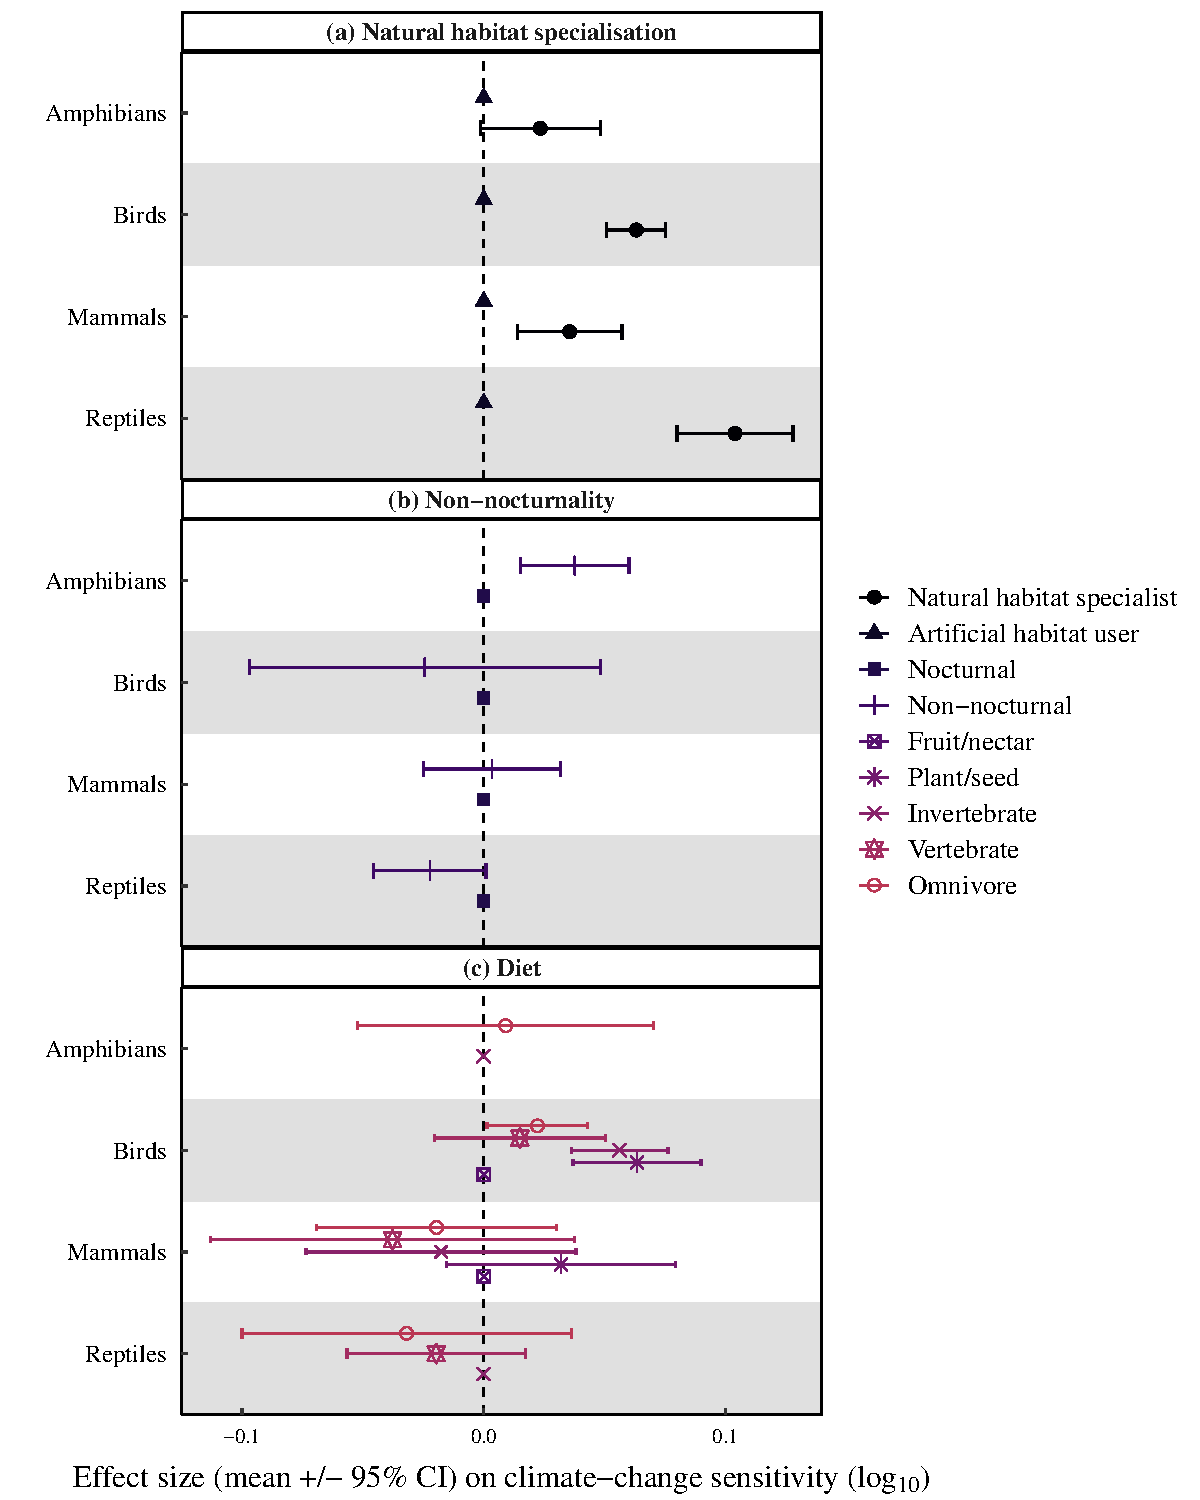
\includegraphics[scale=0.75]{figures/Chapter4/Figure5_V2}
\caption[Estimated effects of the categorical traits on climate-change sensitivity, from the PGLS models fitted in each class.]{\textbf{Estimated effects of the categorical traits on climate-change sensitivity, from the PGLS models fitted in each class (mean effect $\pm$ 95\% confidence interval).} For each categorical trait, I show the effect size for all levels referring to the reference level (vertical dashed line). \textbf{(a)} For artificial habitat use, the reference level is `Artificial habitat user'; \textbf{(b)} for diel activity, the reference level is `Nocturnal'; \textbf{(c)} for diet, the reference level for mammals and birds is `Fruit/nectar' eaters, but it is `Invertebrate' eaters for amphibians and reptiles. }
\label{chap4_fig5}
\end{figure}


\clearpage
%% Figure climate-change sensitivity - continuous predictors
\begin{figure}[h!]
\centering
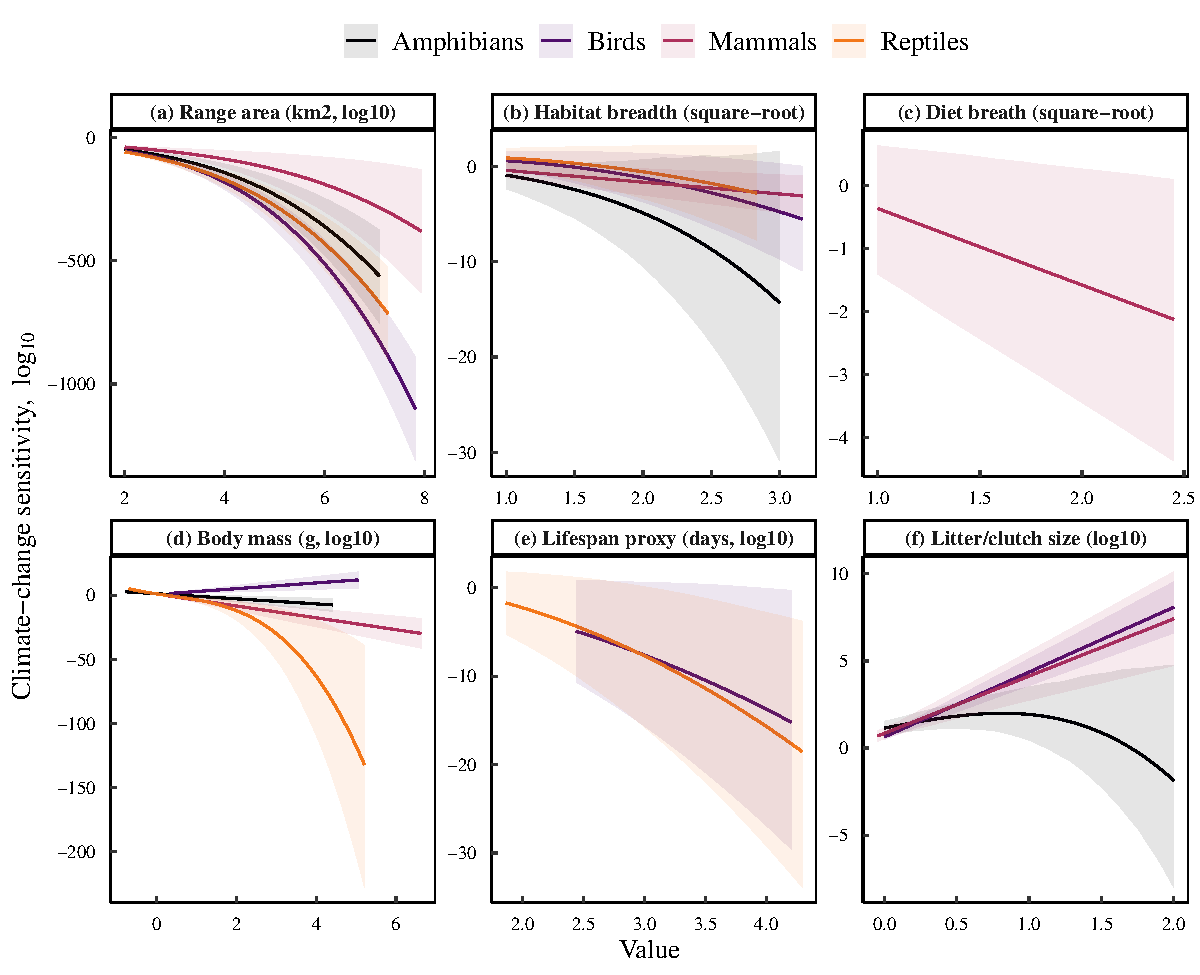
\includegraphics[scale=0.7]{figures/Chapter4/Figure6}
\caption[Effects of the continuous ecological characteristics on climate-change sensitivity, estimated from the PGLS models in each class.]{\textbf{Effects of the continuous ecological characteristics on climate-change sensitivity, estimated from the PGLS models in each class.} The lines represent the estimated relationships between climate-change sensitivity and ecological characteristics; the shaded areas are 95\% confidence intervals. I plotted the estimated relationships only when they were found to be significant.}
\label{chap4_fig6}
\end{figure}

\subsubsection{Robustness of the PGLS models}
The PGLS models were robust to distributional assumptions (Figures \ref{SI_4_Figure18}-\ref{SI_4_Figure21}). When fitting the models on all species (including those with range area $\leq$100km$^2$), I found that the relationship between climate-change sensitivity and geographical range area was reversed in all classes (with smaller-ranging species estimated to be less sensitive). This result is likely an artefact caused by the underestimation of climate-change sensitivity for the most narrow-ranging species, which would support the exclusion of such species from the analysis. Other results were generally not sensitive to the exclusion of species whose range area was $\leq$100 km$^2$ (Figure \ref{SI_4_Figure22}; models' summaries shown in Tables \ref{SI_4_Table17}-\ref{SI_4_Table20}).

Running the models again using data subsets for which I had empirical, non-imputed values only for the ecological characteristics showed that the conclusions of this work are likely robust to imputation uncertainty. Overall, across all classes, the associations of geographical range area, habitat breadth and use of artificial habitats with sensitivity to climate change and land use were consistent with the main models (Tables \ref{SI_4_Table22}-\ref{SI_4_Table26}; Figure \ref{SI_4_Figure23}).


\clearpage


%% ANOVA table for PGLS models
\begin{table}[h!]
\centering
\caption[ANOVA summaries for the PGLS models investigating the associations between the species-level ecological characteristics and species' estimated climate-change sensitivity.]{\textbf{ANOVA summaries for the PGLS models investigating the associations between the species-level ecological characteristics and species' estimated climate-change sensitivity.}}
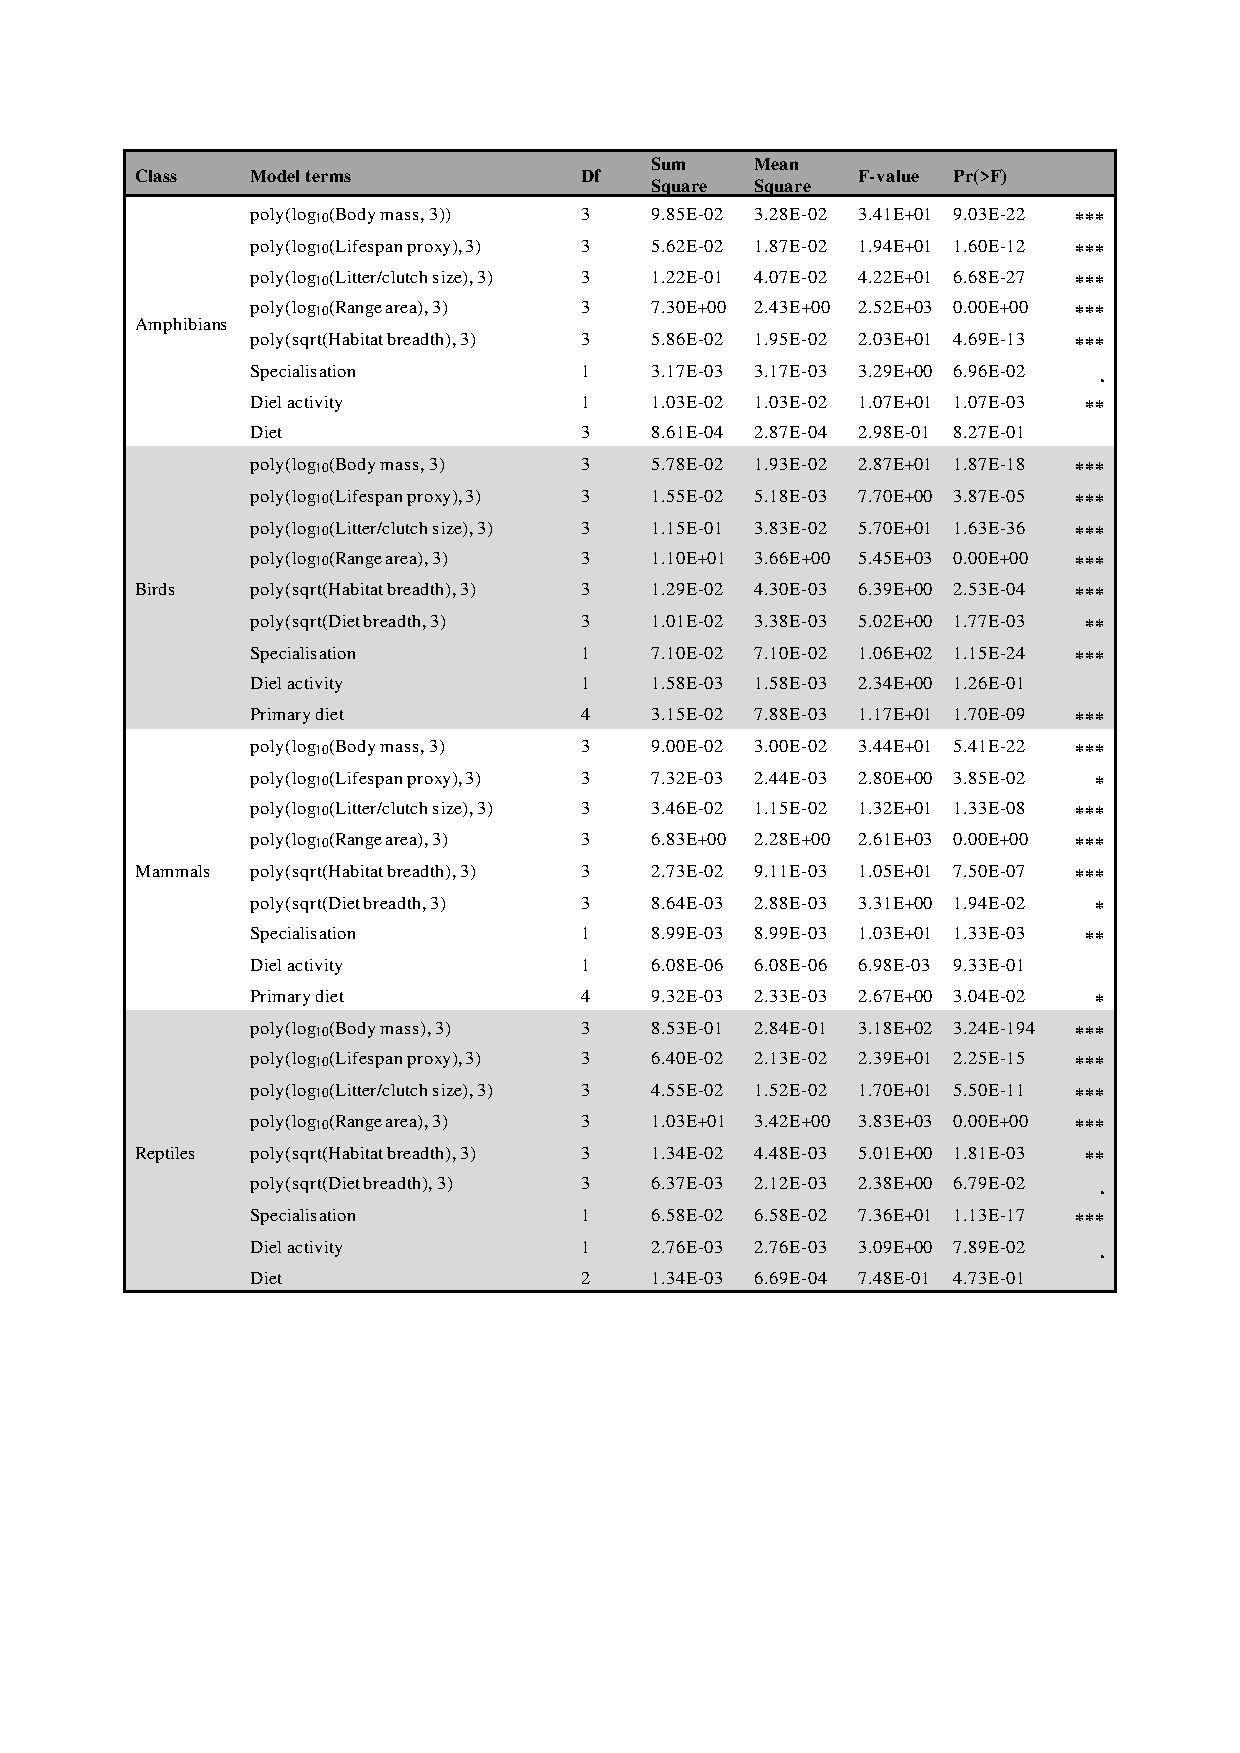
\includegraphics[scale=1, trim={2cm 5 1 2cm}, clip]{figures/Chapter4/Table_ANOVA_PGLS_pdf}
\label{chap4_table2}
\end{table}



\clearpage

\section{Discussion}
Here, I investigated whether species' ecological characteristics were associated with species' sensitivity to two human pressures (climate change and land-use change), across terrestrial vertebrate classes. Overall, I found that geographical range area, habitat breadth and specialisation on natural habitats were the only characteristics that showed consistent effects across both pressures and across the terrestrial vertebrate classes: narrower ranges, narrower habitat breadth and inability to exploit artificial habitats were associated with more negative land-use responses and with higher climate-change sensitivity. My results are in line with previous metanalyses that have found species' extinction risks to be associated with habitat breadth and range area \citep{Chichorro2019}, range shifts under contemporary climate change to be associated with species' historical range limits and habitat breadth \citep{MacLean2017}, and with many other studies on land-use responses or extinction risks \citep{Ripple2017, Newbold2018a, Nowakowski2017}. However, to the best of my knowledge, this work constitutes the first global study to compare patterns among vertebrate classes and between the two major human pressures of climate change and land use. The results of this Chapter have important implications for conservation, as they mean that land-use and climate change are non-randomly affecting all terrestrial vertebrates, with a consistently higher risk for geographically rarer species and habitat specialists. Geographical rarity has been employed by the IUCN for many years in vulnerability assessments \citep{Rodrigues2006}, and this work provides further support for its integration in large-scale assessments. My results also lend support to the idea that habitat specialisation is a likely indicator of species' sensitivity to both land-use and climate change across all vertebrates, thus indices reflecting habitat specialisation should be highly relevant to consider in large-scale vulnerability assessments, such as in \citet{Foden2013}. 

This work further highlights the class-specific associations between most traits and likely responses to human-driven environmental changes, but again highlighting a non-random reshaping of vertebrate biodiversity under global changes. In the case of land use, I find that the directionality of the responses not only often depends on taxonomic class but also on land-use type, further complicating the patterns. In line with past work highlighting the low explanatory power of traits when used to explain species' responses to human pressures \citep{Angert2011, Verberk2013, Cannistra2021}, I found that most traits explained a small proportion of the interspecific variation in land-use responses and in climate-change sensitivity. The only exception was range area, which explained a large proportion of the interspecific variation in climate-change sensitivity. Given that the estimates of climate-change sensitivity were based on properties of species' climatic niches \citep{Rinnan2019}, it was not surprising that range area explained such an important part of the interspecific variation in climate-change sensitivity, as it is likely that broader range areas are associated with broader climatic tolerances, and thus with lower estimated climate-change sensitivity on average.

Despite their generally low explanatory power, traits have been used to assess species vulnerability to human threats, in particular to climate change \citep{Foden2013, Bohm2016}. One of the conceptual appeals behind the use of traits is that if clear patterns in responses to environmental change can be identified across taxa, then it could be possible to generalize their effects in space and time \citep{Verberk2013, Hamilton2020}, which is of interest for conservation -– notably for data deficient species and/or those lacking estimates of abundance or population sizes. This work does not provide support for the generalisation at large scales of the effects of life-history and dietary traits on sensitivity to either land-use or climate change. The class-specific influence of traits on climate-change sensitivity, coupled with their low explanatory power, could be one of the reasons why trait-based approached have been shown to perform less well and show less congruence than trend-based approaches (which rely on the use of long-term population data) for climate-change vulnerability assessments \citep{Wheatley2017}. I would like to emphasize that this does not mean that life-history and dietary traits are unimportant for understanding species' responses, but it means that their effects and relative importance could depend on interactions between the considered taxa and the pressures affecting them.  

Further, it is possible that general underlying patterns remain undetected or are being masked by interactions and trade-offs among traits, which I did not consider here. For instance, larger species tend to have larger dispersal distances and movement abilities \citep{Jenkins2007}, which could be beneficial to resource acquisition in disturbed areas \citep{Hillaert2018}; however, such species also tend to have higher energetic requirements \citep{White2011} and lower reproductive output, which could be detrimental to their persistence in the face of environmental change. Interactions and trade-offs among traits have been shown to be important for understanding which species are likely to persist in disturbed environments \citep{Sayol2020}, but little is known about their potential effects at large scales and for different types of pressure. Thus, developments of my work could focus on the effects of trait interactions on species' sensitivity to climate change and land-use responses. I was also unable to consider intraspecific variation in this work. Intraspecific variation and potential for acclimation and evolutionary adaptation are likely important determinants of species' ability to cope with human disturbance \citep{Carlson2014, Rohr2018}, but considering such effects at large scales is challenging because of the lack of available data.  

Moreover, I investigated climate-change sensitivity and land-use responses separately, meaning that I did not consider the combined effects of these pressures. However, human pressures act in combination \citep{Segan2016, Harfoot2021, Capdevila2022b}, and a number of confounding factors and threats that I could not account for could possibly influence species' sensitivity. For example, larger species might be more sensitive to warming than smaller species \citep{Merckx2018, Hantak2021}, but they could also be better able to persist in fragmented landscapes, such that habitat fragmentation and climate warming may have opposite effects on the responses of such species. Further, larger species might also be disproportionally exposed to other threats such as overexploitation and human-wildlife conflicts \citep{Ripple2014, Ripple2017}. Interactions among traits, among types of pressure, and among traits and pressures should ideally be considered together to understand species' responses to human disturbances \citep{Hantak2021}. However, considering all these effects simultaneously may be challenging because of data-limitation issues, model complexity, and difficulty in assessing and disentangling individual and interactive effects. In addition, I would like to emphasize that my results, based on correlative assessments of the associations between ecological characteristics and species' sensitivity to climate change and species' land-use responses, do not allow to infer any causal links between traits and species' responses to global changes. Reinforcing our mechanistic understanding of how traits influence species' ability to cope with different disturbances may help understand opposite signatures of human impacts on vertebrate trait diversity. Further work could help elucidate the mechanistic links between species traits and responses to environmental change, perhaps supported by long-term population data and demographic models \citep{HernandezYanez2022}.

To conclude, the results of this Chapter indicate that land-use and climate change are likely to impact terrestrial vertebrates non-randomly with respect to their ecological characteristics, which could have important consequences for ecosystem functioning \citep{Duffy2003, Luck2012}. For instance, I detected substantial declines in occurrence probability of certain dietary groups in disturbed land-use types, most notably invertebrate eaters and fruit/nectars eaters in all classes. I also found higher climate-change sensitivity for invertebrate- and plant/seed-eating birds. My findings thus highlight the potential risks from global changes for ecosystem processes and services sustained by those species, such as pest control, seed dispersal or pollination \citep{Civantos2012, GonzalezVaro2013, Fricke2022}, highlighting the need to put into place mitigation and conservation measures in the face of global changes. 


\chapter{General Discussion}

\chapter{Conclusion}


\clearpage
\addcontentsline{toc}{chapter}{Bibliography}
\chapter*{Bibliography}
\renewcommand{\baselinestretch}{1}
\printbibliography[heading=none]

%%%%%%%%%%%%%%%%%%%%%%%
%% APPENDICES %% Structured by chapters

% line spacing
\renewcommand{\baselinestretch}{1.15}

% figure and section numbering -- start with S for the appendices

\clearpage

\addcontentsline{toc}{chapter}{Appendices}
\chapter*{Appendices}
\clearpage

\addcontentsline{toc}{chapter}{Appendix 1: Supporting information for Chapter 1}
\chapter*{Appendix 1: Supporting information for Chapter 1}

\addcontentsline{toc}{chapter}{Appendix 2: Supporting information for Chapter 2}
\chapter*{Appendix 2: Supporting information for Chapter 2}
\renewcommand{\thefigure}{S2.\arabic{figure}}
\renewcommand{\thetable}{S2.\arabic{table}}
\renewcommand{\thesection}{S2.\arabic{section} }
\section{Taxonomic corrections}
Across the different sources, similar species could appear under different binomial names. This was a problem when matching datasets by species. Moreover, it is possible that within a source, a given species was appearing under two or more different, synonymic names. As such, taxonomic synonymy created duplicated rows for the same species, overall falsely increasing the total number of species and potentially inflating the number of missing trait values. Taxonomic synonymy was hence a major issue. Due to the large number of species across datasets, extensive manual checks could not be applied. The presence of typos in species names had the same effect as synonymy, erroneously duplicating species. We attempted to correct for taxonomy first by correcting for typos, and second by identifying species which were entered under non-accepted names and replacing these with the accepted name. To this end, we developed an automated procedure, complemented with a few manual entries where errors were opportunistically spotted. Such errors in taxonomy were notably spotted when attempting to retrieve trait data for subsets of species, for analyses unrelated to the work conducted here. Taxonomic synonymy was as such checked manually for 91 species (56 birds, 7 mammals and 28 reptiles); in that case, information was extracted from other diverse sources (such as the Reptile Database (\url{http://www.reptile-database.org/}); Avibase (\url{https://avibase.bsc-eoc.org/avibase.jsp?lang=EN\&pg=home}); AmphibiaWeb (\url{https://amphibiaweb.org/}); and additional manual checks using the IUCN Red List for mammals). A column in the Synonym dataset mentions where manual checks were applied (in which case the Synonym dataset was manually corrected). 


\subsection*{Automated procedure and outputs.}
\paragraph{Extracting names from the IUCN Red List and the Integrated Taxonomic Information System (ITIS).}
The objectives of the automated procedure were to (1) extract species synonymic binomial names from the IUCN Red List or from ITIS (using the rredlist \citep{rredlist} and taxize \citep{Chamberlain2013} R packages); and (2) identify the status of each name (accepted or not accepted). We started by generating a list of all names featuring in any of the sources. These `original' names were corrected for typos (using gnr$\textunderscore$resolve function, taxize package). Then, the IUCN Red List was queried and any listed synonyms were stored, as well as the status of each synonym (accepted or not accepted). When species were not found in the IUCN Red List, synonyms were extracted from ITIS. When species were not found in ITIS either, corrected names (original names corrected for typos) were used. Family and order designations were extracted using the same procedure and some entries were retrieved from the Global Biodiversity Information Facility taxonomic backbone when not available in the Red List or in the ITIS (GBIF, \url{https://www.gbif.org/tools/species-lookup}).\\
\textbf{NB:} for species entered with the forms \textit{Genus cf.}, \textit{Genus aff.} or \textit{Genus spp.}, the accepted binomial name was left empty.

\paragraph{Output.} We generated a `Synonym' dataset containing records of all names (for 14124, 8743, 6090, and 11678 binomial names for birds, amphibians, mammals and reptiles respectively), their status and their potential synonyms.

\paragraph{Harmonising taxonomy in trait datasets.}
Taxonomy across datasets was finally homogenised by replacing synonyms with a uniquely identified accepted name. As a consequence, the total number of identified unique species decreased (Figure \ref{SI2_taxcor} A). The species presenting the highest number of synonyms was the East African mole rat (\textit{Tachyoryctes splendens}), for which we found 12 synonymic names (Figure \ref{taxcor} B).

% figure: distribution of names and differences in species number
\vspace{0.5cm}
\begin{figure}[h!]
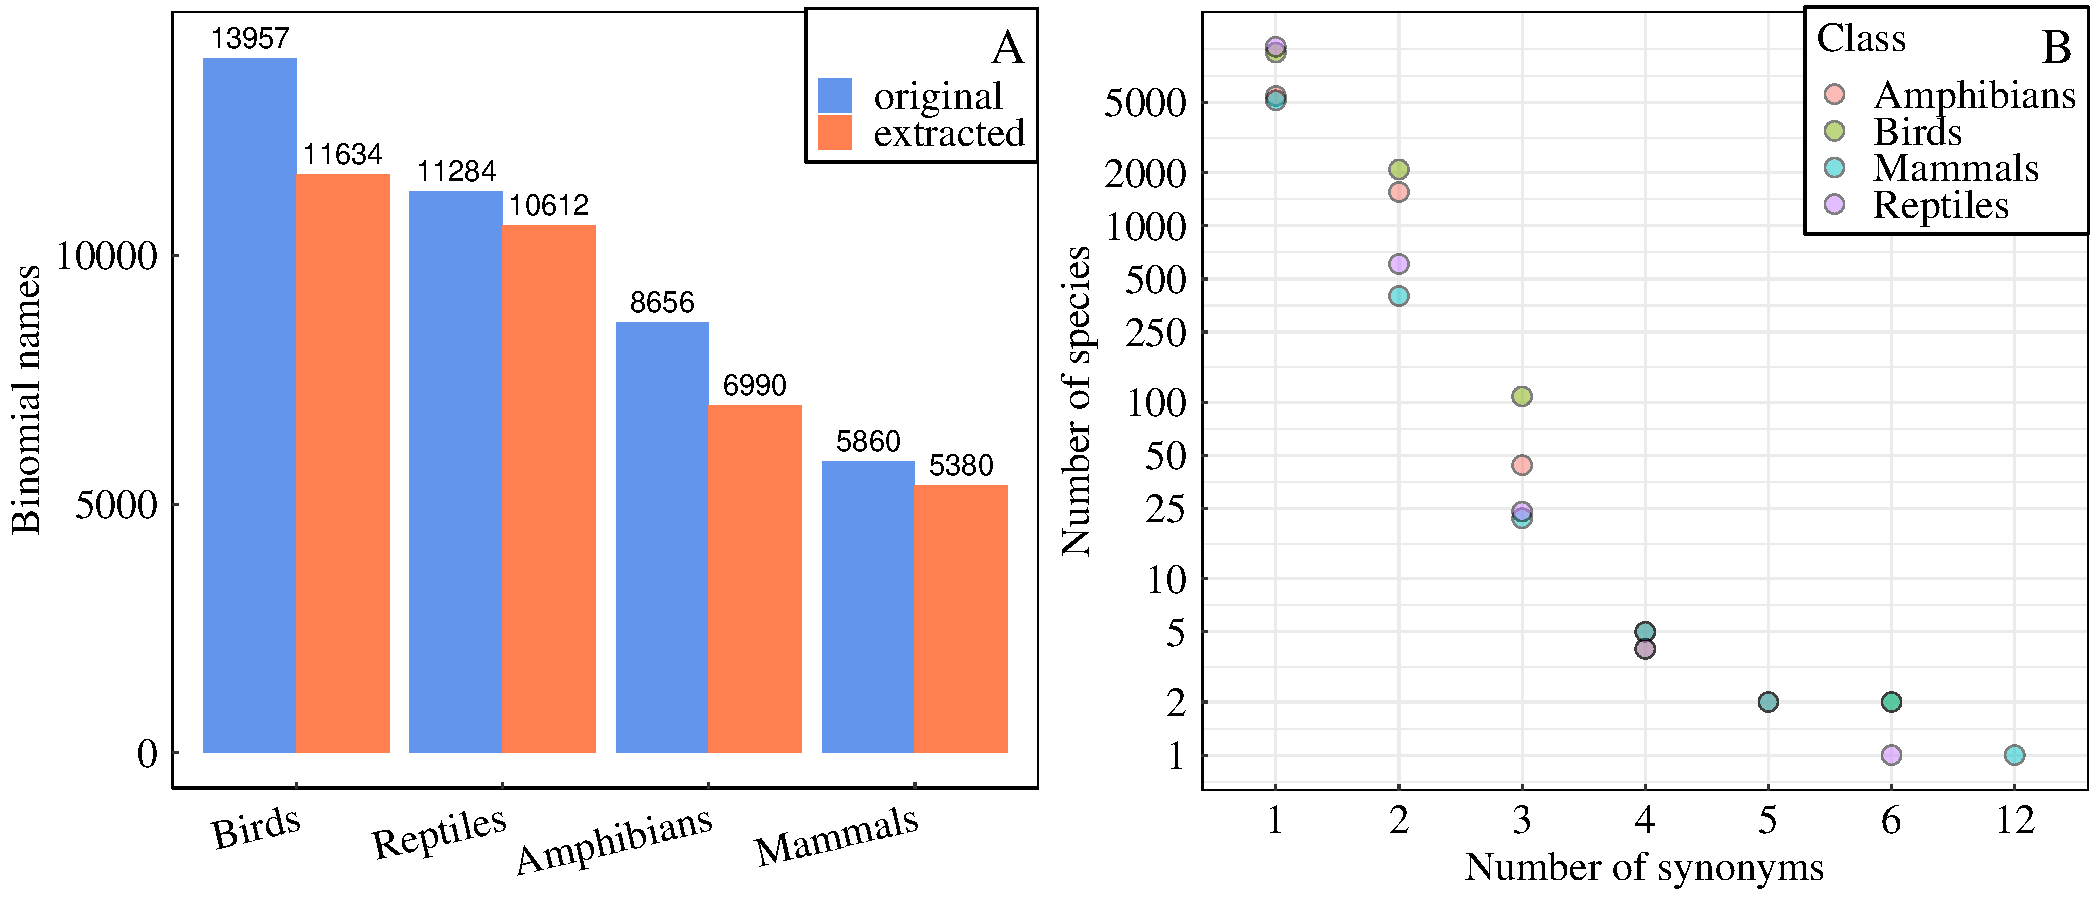
\includegraphics[scale=0.45]{Supporting/Chapter2/Figures/tax_corrections}
\caption[Difference in species number before and after taxonomic correction (A) and distribution of number of synonyms across datasets (B)]{\textbf{Difference in species number before and after taxonomic correction (A) and distribution of number of synonyms across datasets (B).} \textbf{(A)} shows the number of species (binomial names) extracted from all sources (blue bars), and the number of uniquely identified accepted names (in red). Replacing non-accepted synonyms by one identified accepted name reduced the number of species in all classes, with the largest reduction for birds. \textbf{(B)} shows the distribution of the number of synonymic names. In all four classes, more than 5,000 species were known under one name only. Nevertheless, a large number of species had two identified synonyms (range: 400 species for mammals - 2086 for birds). The most potentially replicated species was the East African mole rat \textit{Tachyoryctes splendens}, for which 12 synonyms were identified.}
\label{SI2_taxcor}
\end{figure}

%Decrease by 2,323 unique binomial names for birds. The diminution was of 632 unique identified species for reptiles, of 1,666 for amphibians and of 488 for mammals.

The automated procedure was not perfect, and taxonomic errors are likely to have persisted in the trait datasets. The Red List and the ITIS were not comprehensive taxonomic sources, and for clades with high degrees of synonymy in names, such as reptiles or amphibians, neither the Red List or the ITIS contained enough information.Taxonomy may be further improved by using class-specific sources in an automated procedure. 

\clearpage

\section{Additional information for trait compilation}

\begin{comment}
\subsection{Data sources for the `Senior' dataset}

\cite{Anderson1999} \\
\cite{Ao2003} \\
\cite{Arroyo2008} \\
\cite{Bain2004}\\
\cite{Barrio-Amoros2012}\\
\cite{Bennett1999} \\
\cite{Bernarde2009} \\
\cite{Blomquist2009} \\
\cite{Brasileiro2005} \\
\cite{Campbell1998} \\
\cite{Caramaschi1997} \\
\cite{DaSilva2009}\\ 
\cite{DeAlmeidaPrado2000} \\
\cite{DeAlmeidaPrado2003} \\
\cite{DeCarvalho2010} \\
\cite{Fouquet2007} \\
\cite{Goldberg2008} \\
\cite{Gonzalez2008} \\
\cite{Guayasamin2006} \\
\cite{Hertz2012}\\
\cite{Heyer1994} \\
\cite{Heyer1996} \\
\cite{Heyer2002} \\
\cite{Ibanez2012}\\
\cite{Jared2011} \\
\cite{Jungfer2002} \\
\cite{Kan2010} \\
\cite{Lance1993} \\
\cite{Lynch1989} \\
\cite{Matson1990} \\
\cite{McCranie1993} \\
\cite{Ningombam2007} \\
\cite{Ohler2011} \\
\cite{PombalJr.2011} \\
\cite{Savage2002} \\
\cite{Shahriza2010} \\
\cite{Shepard2005}\\
\cite{Simoes2010} \\
\cite{Stuart2006} \\
\cite{Su2005} \\
\cite{Sunyer2009} \\
\cite{Wollenberg2006} \\
\cite{Zimmermann1983} \\
\cite{Zug1979}\\
http://amphibia.my/\\
http://amphibiaweb.org/

\end{comment}


\subsection*{Correlations among closely related traits}

% Amphibians: body mass VS body length and Maturity VS longevity
\begin{figure}[h!]
\centering
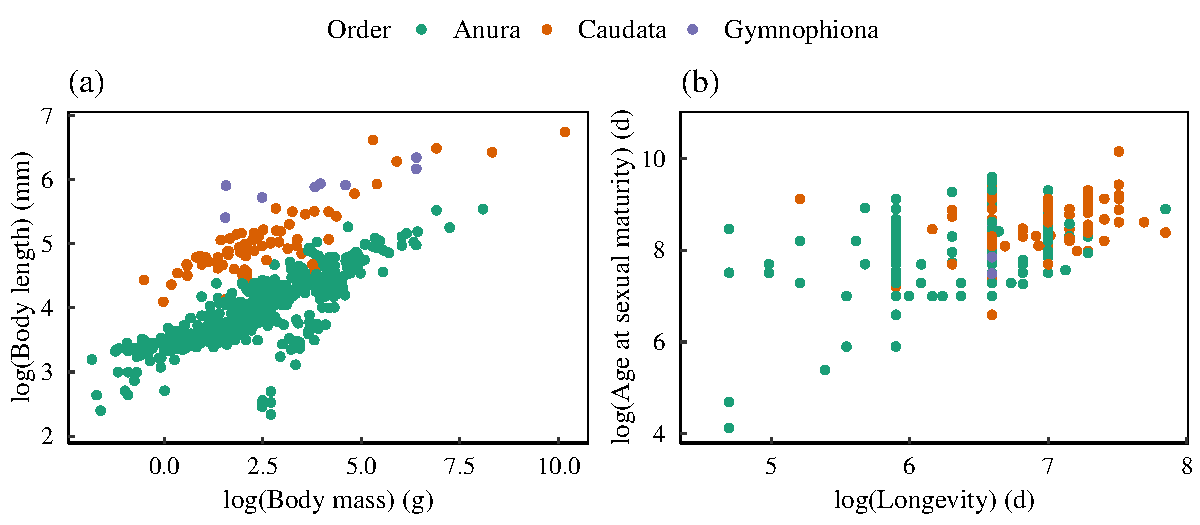
\includegraphics[scale=0.85]{Supporting/Chapter2/Figures/Correlations/MatLong_BMBL_amphibians}
\caption[(a) Body mass versus body length and (b) Longevity versus age at sexual maturity in amphibians.]{\textbf{(a) Body mass versus body length and (b) Longevity versus age at sexual maturity in amphibians.} The Pearson's correlation coefficient was 0.71 in (a) and 0.55 in (b) (order was not included in these coefficients).} 
\label{}
\end{figure}

% Birds: Longevity VS Generation length
\begin{figure}[h!]
\centering
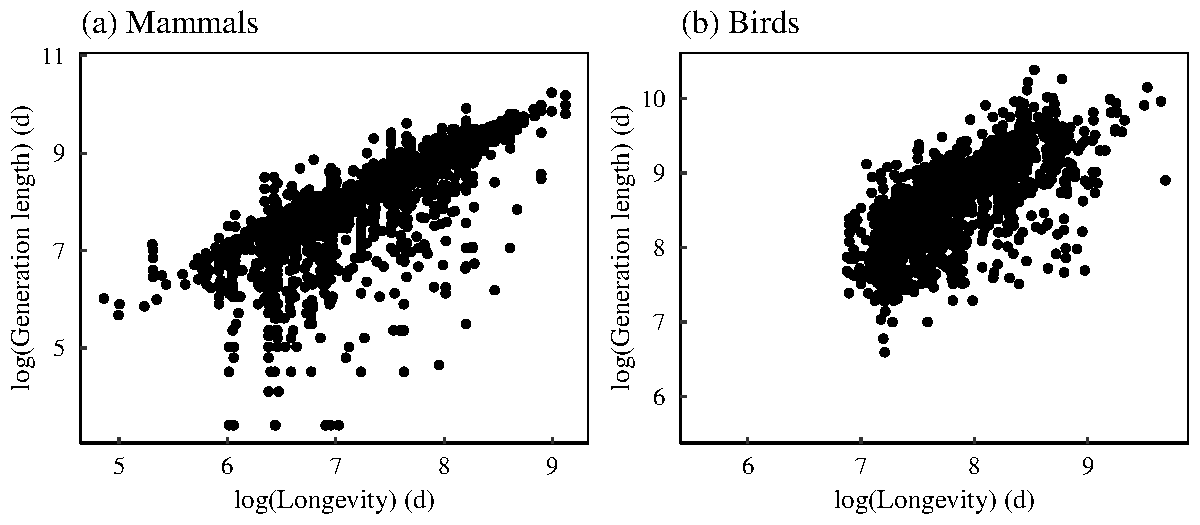
\includegraphics[scale=0.85]{Supporting/Chapter2/Figures/Correlations/GL_Longe_birds_mammals}
\caption[Generation length versus longevity data in birds.]{\textbf{Generation length versus longevity data in mammals and birds.} The Pearson's correlation coefficient was 0.74 in (a) and 0.70 in (b).} 
\label{}
\end{figure}

\pagebreak

\begin{comment}
\subsection{Habitat affinities and use of artificial habitats}

\paragraph{Habitat breadth.}
The IUCN Red List habitat data records habitat types in which species are found to occur. Habitats are classified into 96 categories, which we pooled into 13 broader habitat variables: 
Forest, Savanna, Grassland, Shrubland, Wetland, Rocky areas, Caves and subterranean, Desert, Marine, Marine intertidal or coastal/supratidal, Artificial, Introduced vegetation and Other/Unknown (level two of the IUCN Habitat Classification Scheme). Species habitat preferences were described using these variables as binary (taking 1 if a species was known to occur in the habitat and 0 otherwise). Habitat breadth was then calculated as the number of habitats recorded to be used by a species. Information regarding habitat suitability and habitat importance is also available in the IUCN Red List habitat data, so it is possible to use a weighted sum to calculate habitat breadth. Weights can be assigned to account for the suitability and importance of each habitat.
%Suitability was classified in three categories in the IUCN Red List: `suitable', `marginal' or  `unknown'. Suitable habitats were recorded to be either of major importance, not of major importance or of unknown importance. We used the weights provided in Table \ref{weights} to produce weighted sums of the number of habitats used by each species. Note that the weighting system used in this work does not impact coverage or completeness (as the amount of information across species remains similar regardless of the weights). Moreover, habitat breadth was not highly sensitive to the choice of weights (see Figure.)

% table of weigths used for habitat breadth calculations
\begin{table}[h!]
\renewcommand{\baselinestretch}{1}
\renewcommand{\arraystretch}{1.5}
\begin{center}\fontsize{9}{11}\selectfont
\caption[Weights used in the calculation of habitat breadth]{\textbf{Weights used in the calculation of habitat breadth.} Habitat breadth was calculated as the weighted sum of the number of habitats used by a species. Weights were assigned to each habitat given its importance and its suitability.} 
\label{weights}
\begin{tabular}{|l|c|c|c|}
\hline
\multicolumn{1}{|c|}{\multirow{2}{*}{\textbf{Suitability}}} & \multicolumn{3}{c|}{\textbf{Major importance}} \\ \cline{2-4} 
\multicolumn{1}{|c|}{}                             & \textbf{Yes}       & \textbf{No}        & \textbf{Unknown}       \\ \hline
\textbf{Suitable}                                           & 1         & 0.5       & 1             \\ \hline
\textbf{Marginal}                                           & NA       & 0.3       & 0.3           \\ \hline
\textbf{Unknown}                                            & NA         & 0.3       & 1             \\ \hline
\end{tabular}
\end{center}
\end{table}

\end{comment}

\clearpage

\section{Cutting distribution maps by altitudinal limits}

\begin{figure}[h!]
\centering
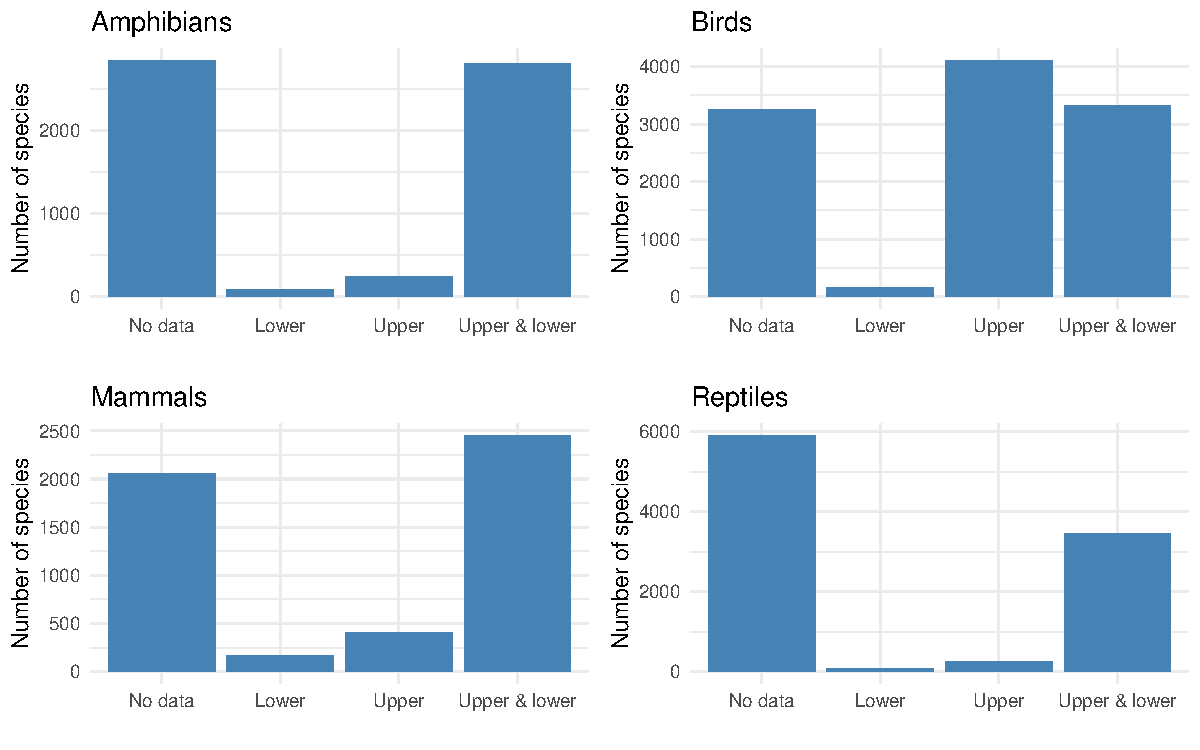
\includegraphics[scale=0.7]{Supporting/Chapter2/Figures/Rangesizes/Elevation_data_amount}
\caption[]{\textbf{Availability of altitudinal limits across species.} Upper and lower altitudinal limits were extracted from the IUCN Red List.}
\label{}
\end{figure}

\begin{figure}[h!]
\centering
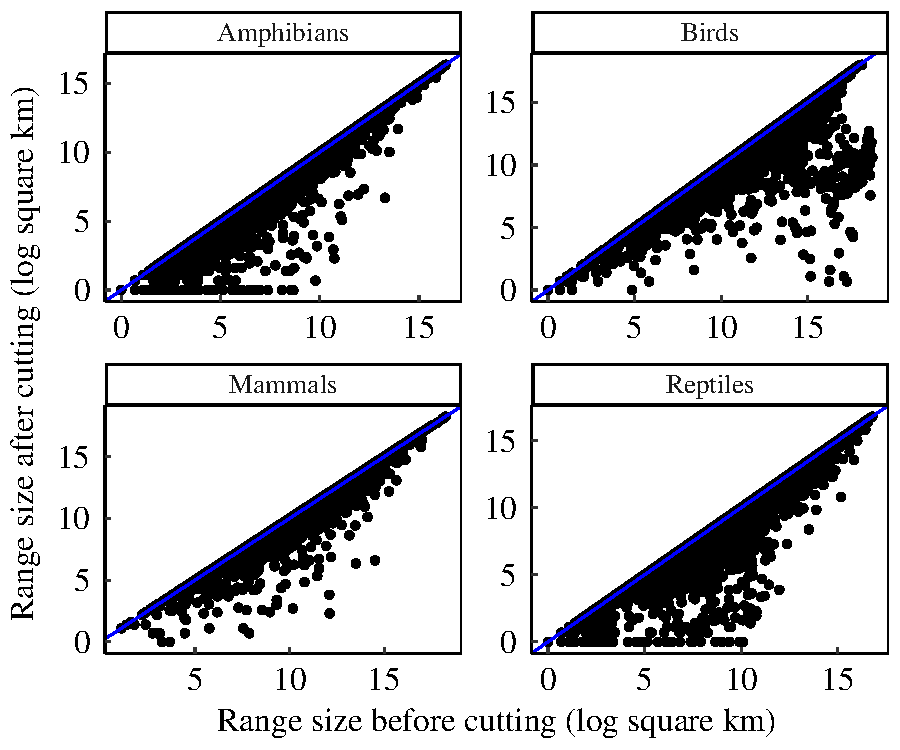
\includegraphics[scale=0.7]{Supporting/Chapter2/Figures/Rangesizes/RangeSizes_before_aftercuts}
\caption[]{\textbf{Range sizes before VS after cutting by altitudinal limits.}}
\label{}
\end{figure}

\pagebreak

\section{Impact of taxonomic corrections of trait coverage}

\begin{figure}[h!]
\centering
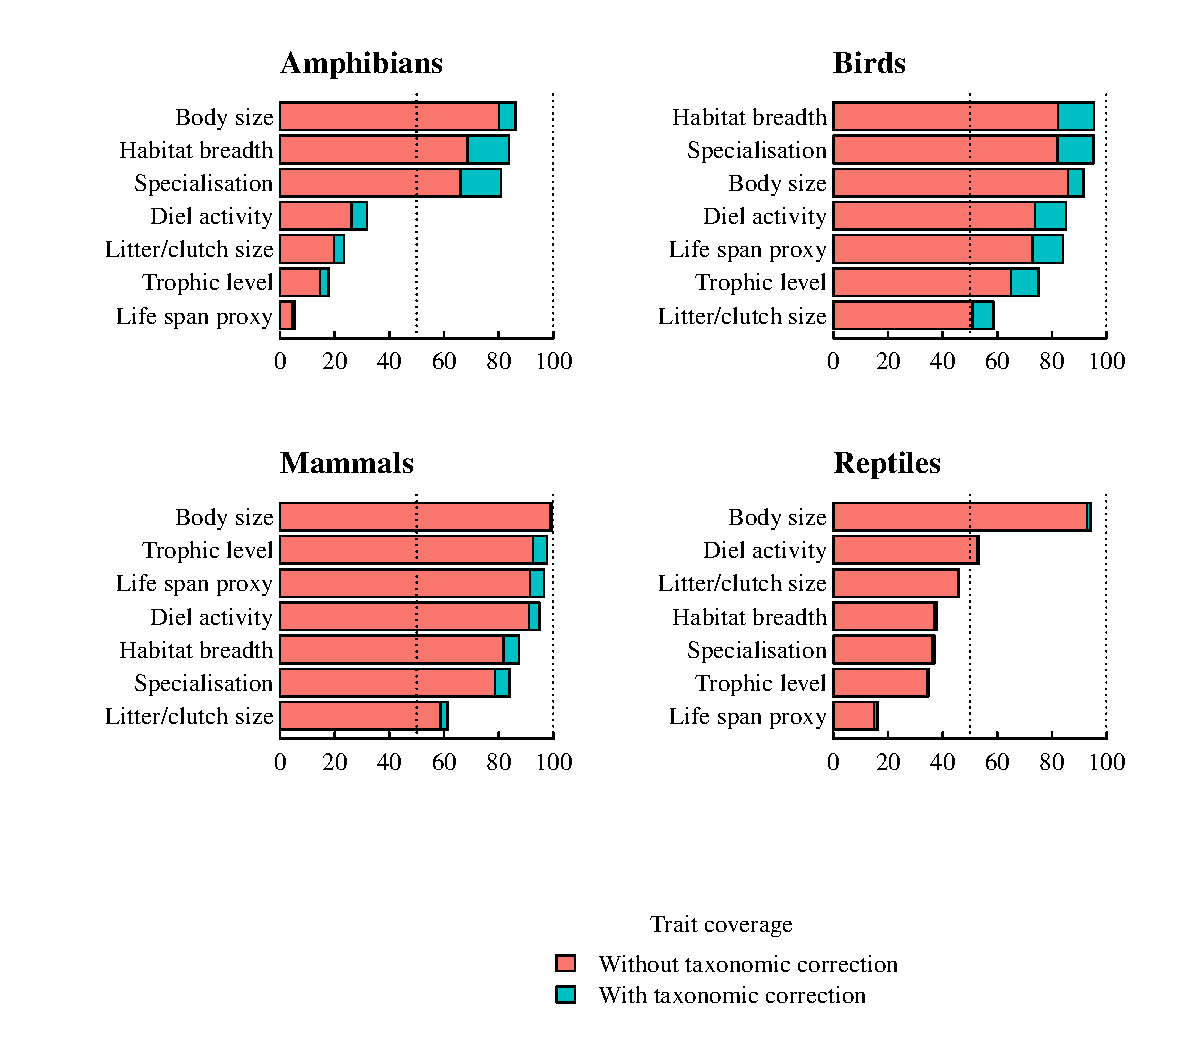
\includegraphics[scale=0.7]{Supporting/Chapter2/Figures/Coverage/DeltaCoverage}
\caption[]{\textbf{Trait coverage when no taxonomic correction is applied before matching sources by binomial names, versus when we apply the described procedure.} Identification of synonyms allowed to increase trait coverage in most cases.}
\label{}
\end{figure}

\newpage
\pagebreak

\section{Assemblage-level median, mean and standard deviation of trait completeness (maps)}

%% Median for all classes
\begin{figure}[h!]
\vspace*{-2cm}
\centering
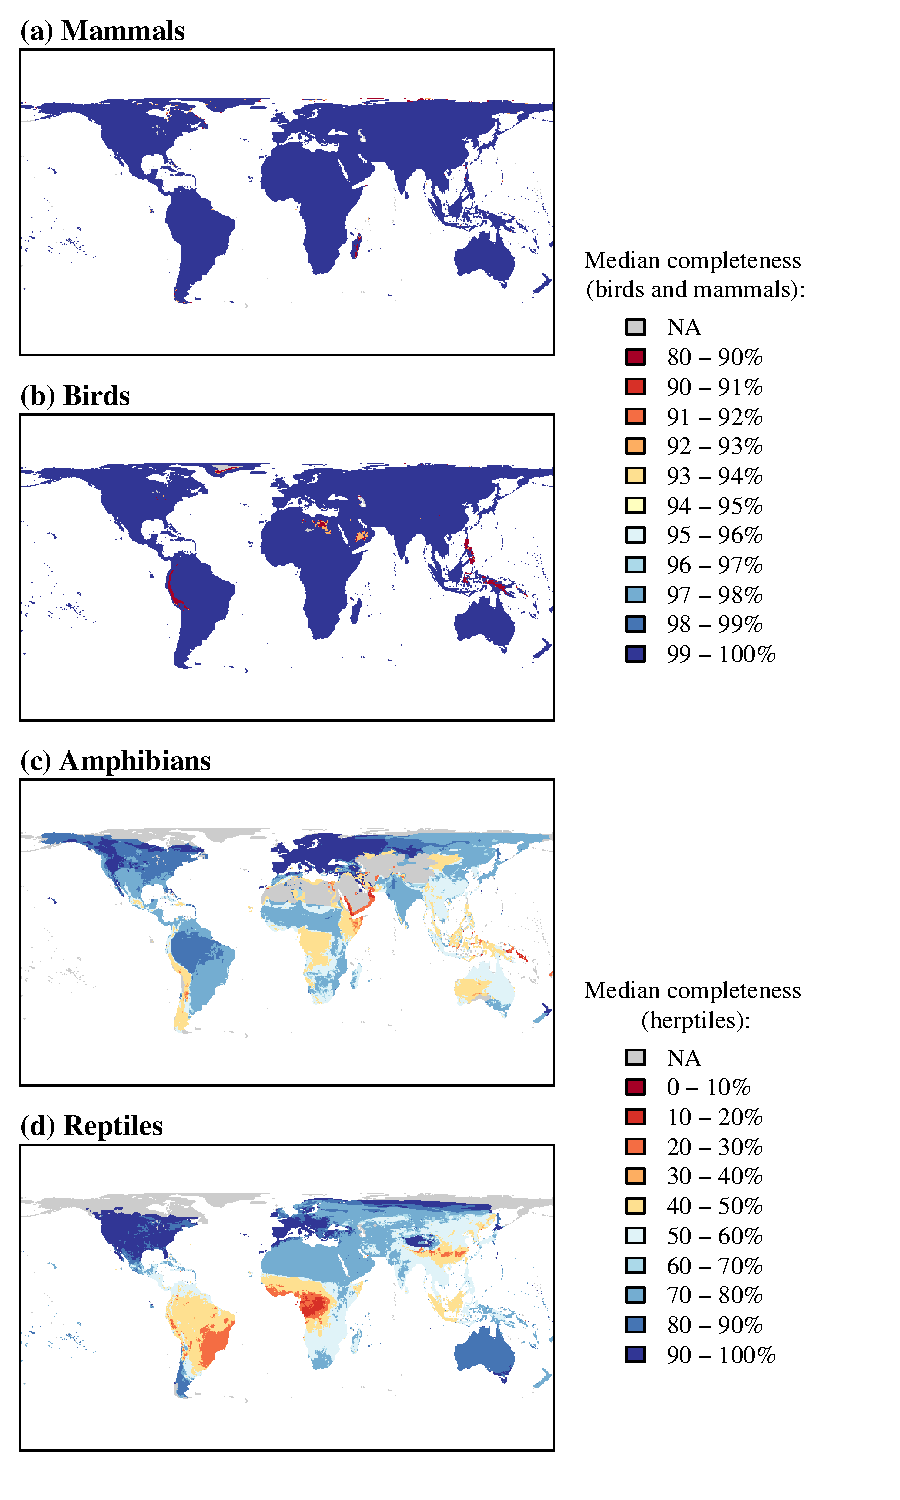
\includegraphics[scale=0.95]{Supporting/Chapter2/Figures/Maps/Median_map}
\caption[Spatial distribution of assemblage-level median trait completeness in herptiles.]{\textbf{Spatial distribution of  assemblage-level median trait completeness.} Note that the color breaks differ for mammals and birds and for herptiles.}
\label{}
\end{figure}

\newpage
%% Mean for all classes
\begin{figure}[h!]
\vspace*{-2cm}
\centering
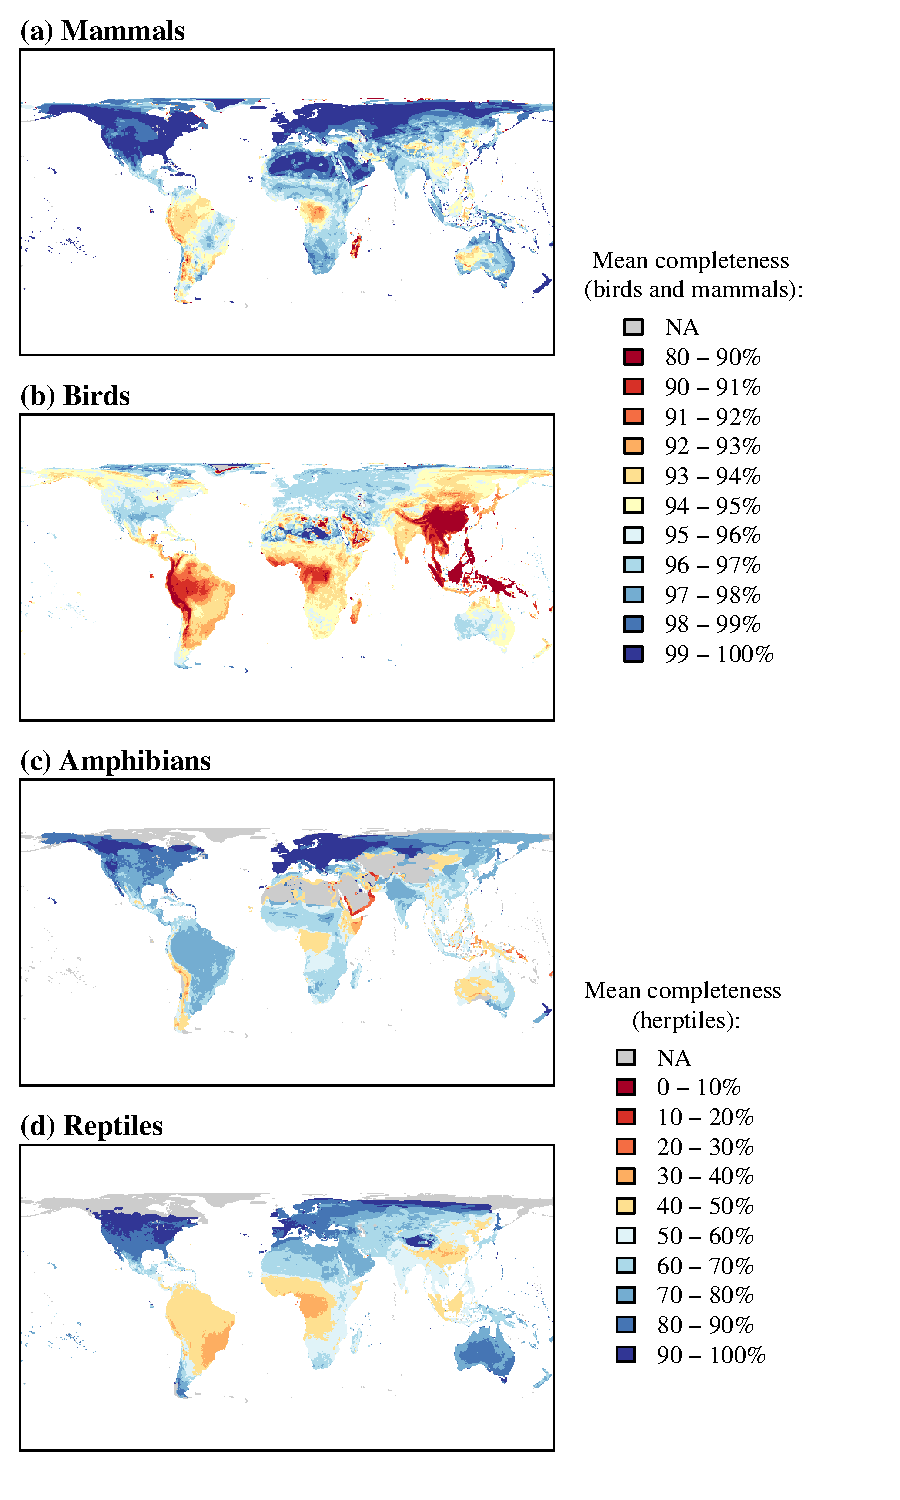
\includegraphics[scale=0.95]{Supporting/Chapter2/Figures/Maps/Mean_map_50k}
\caption[Spatial distribution of assemblage-level mean trait completeness in herptiles.]{\textbf{Spatial distribution of  assemblage-level mean trait completeness.} Note that the color breaks differ for mammals and birds and for herptiles.}
\label{}
\end{figure}

\newpage
%% Standard deviation for all classes
\begin{figure}[h!]
\vspace*{-2cm}
\centering
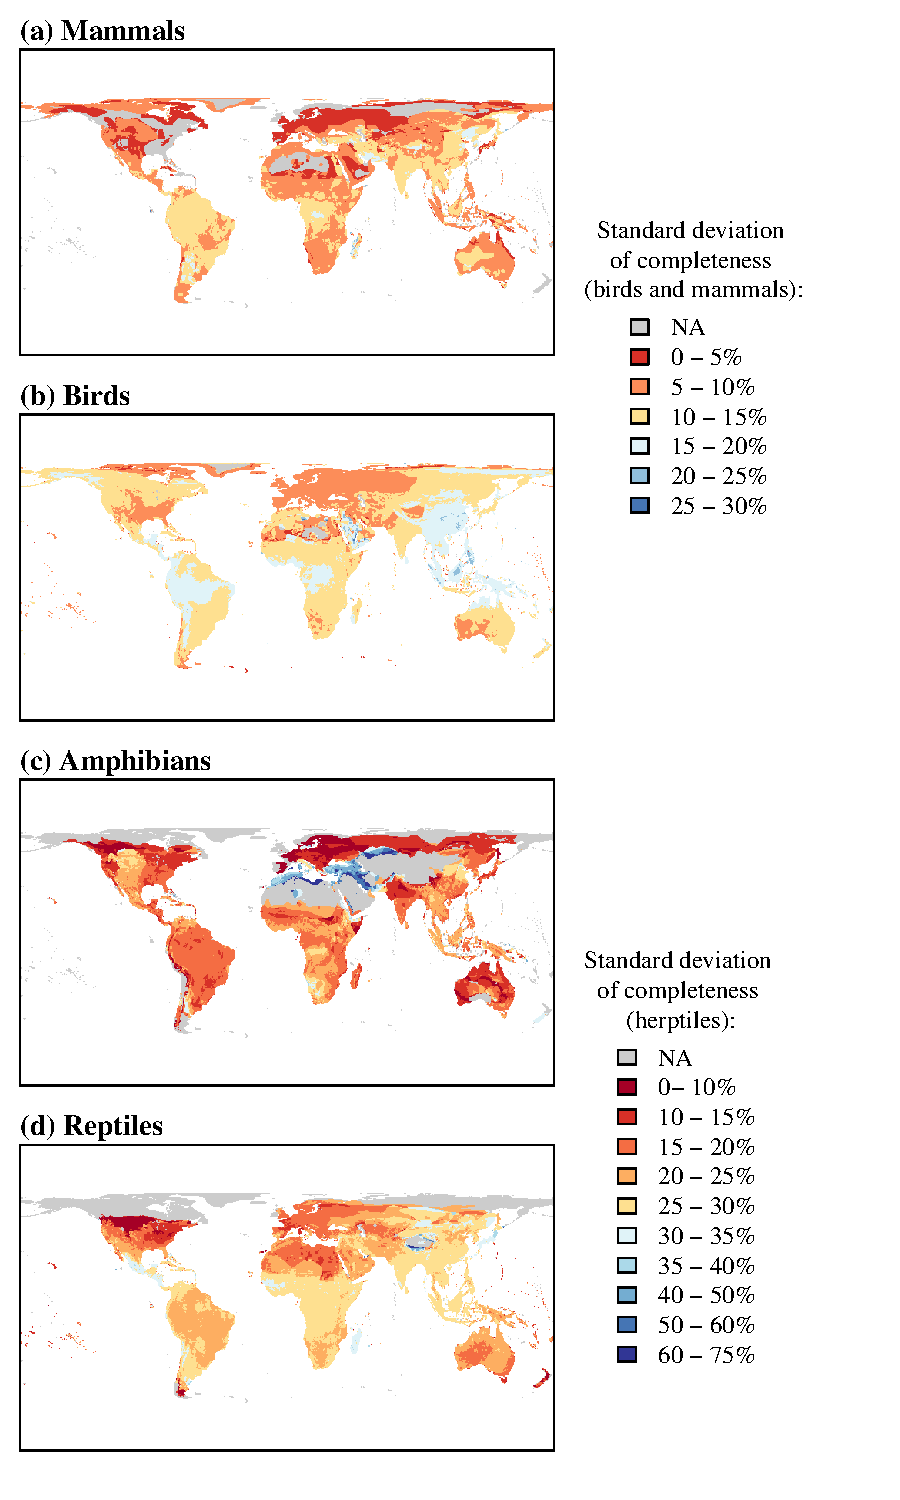
\includegraphics[scale=0.95]{Supporting/Chapter2/Figures/Maps/sd_map}
\caption[Spatial distribution of assemblage-level mean trait completeness in herptiles.]{\textbf{Spatial distribution of  assemblage-level standard deviation of trait completeness.} Note that the color breaks differ for mammals and birds and for herptiles.}
\label{}
\end{figure}


%% SD vs SR
\begin{figure}[h!]
\centering
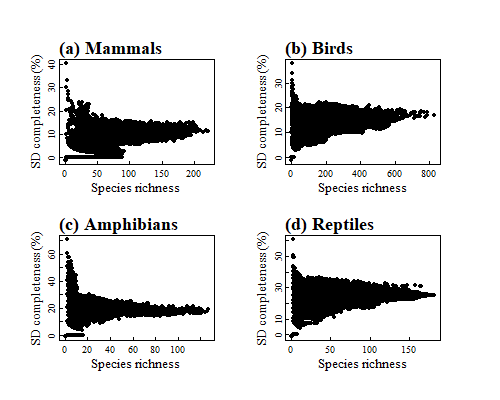
\includegraphics[scale=0.8]{Supporting/Chapter2/Figures/Maps/sd_SR.png}
\caption[]{\textbf{Assemblage-level species richness against standard deviation in completeness.}}
\label{}
\end{figure}

\clearpage
\newpage
\pagebreak

%%%%%%%%%%%%%%%%%%%%%%%%%%%%%%%%%%%%%%%%%%%
\clearpage
\newpage
\pagebreak

\begin{landscape}

\section{Phylogenetic patterns in trait completeness}


\begin{figure}[h!]
\centering
% [scale=1, clip, trim=110 200 100 200] #left bottom right top
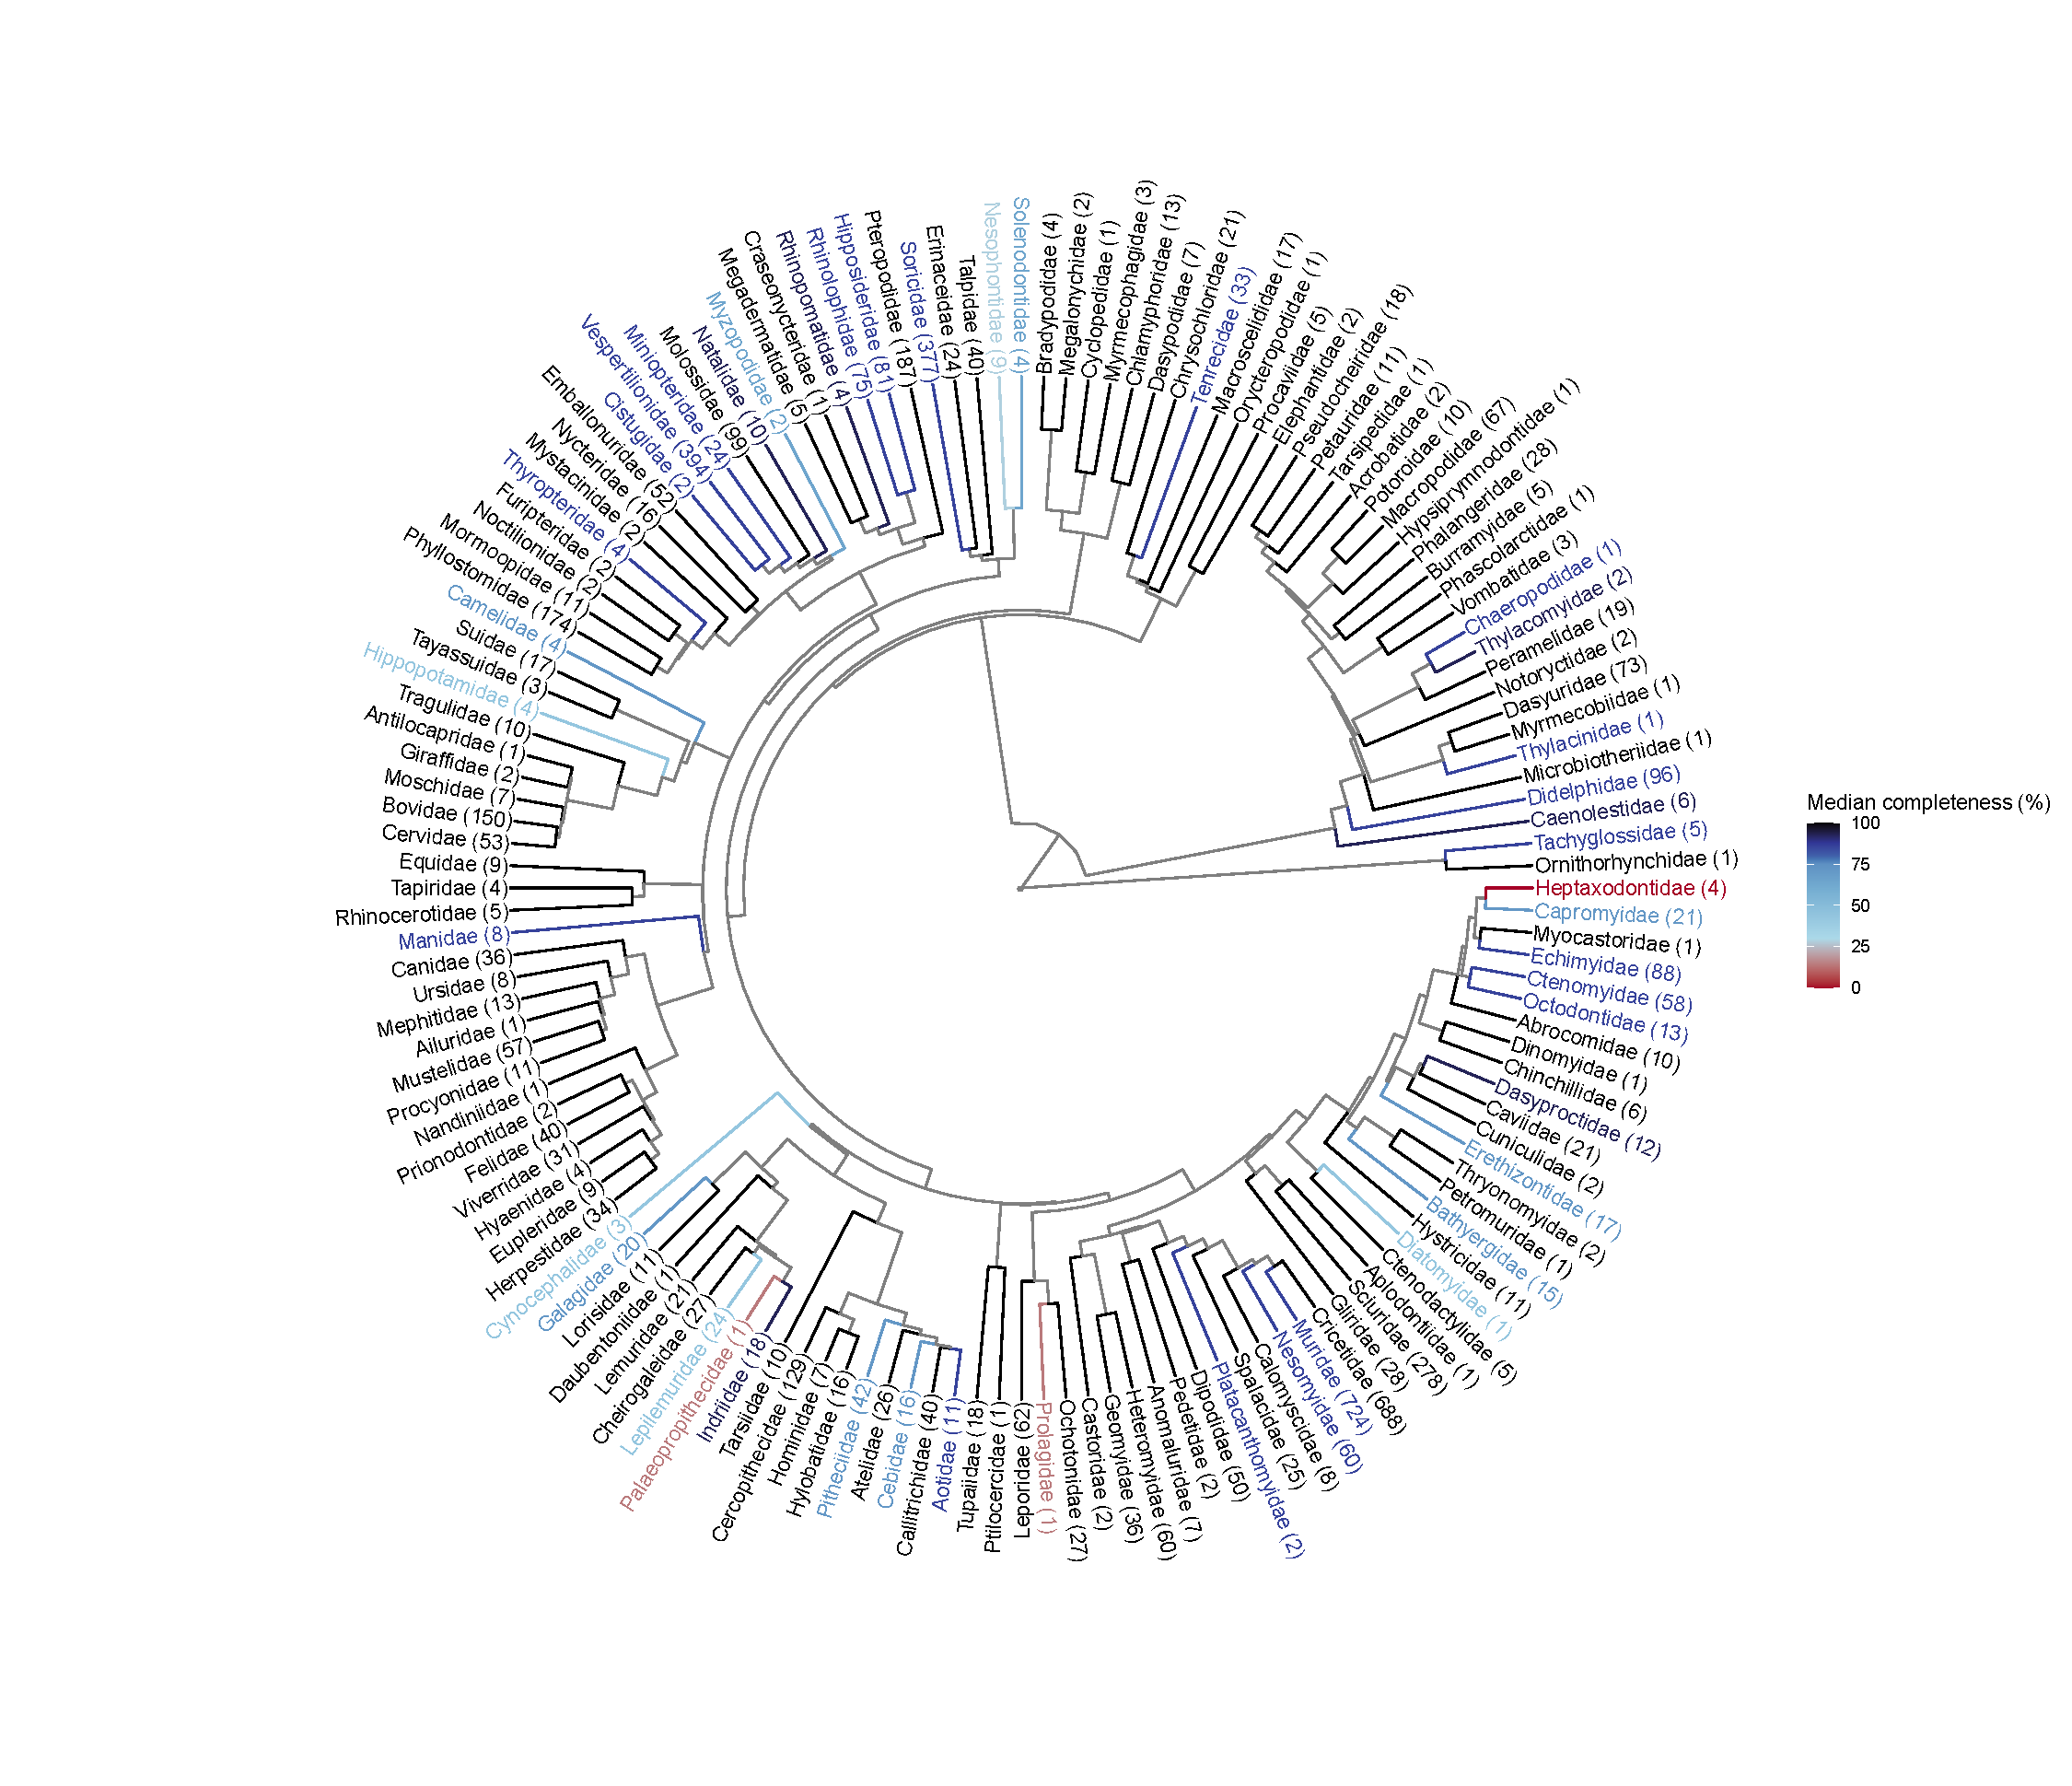
\includegraphics[scale=0.63, clip, trim=100 60 0 60]{Supporting/Chapter2/Figures/Phylogenies/Circular_mammals_V2}
\caption[Within-family median trait completeness in mammals]{\textbf{Within-family median trait completeness in mammals.}}
\label{}
\end{figure}

\newpage
\pagebreak
\vspace{-3cm}

\begin{figure}[h!]
\centering
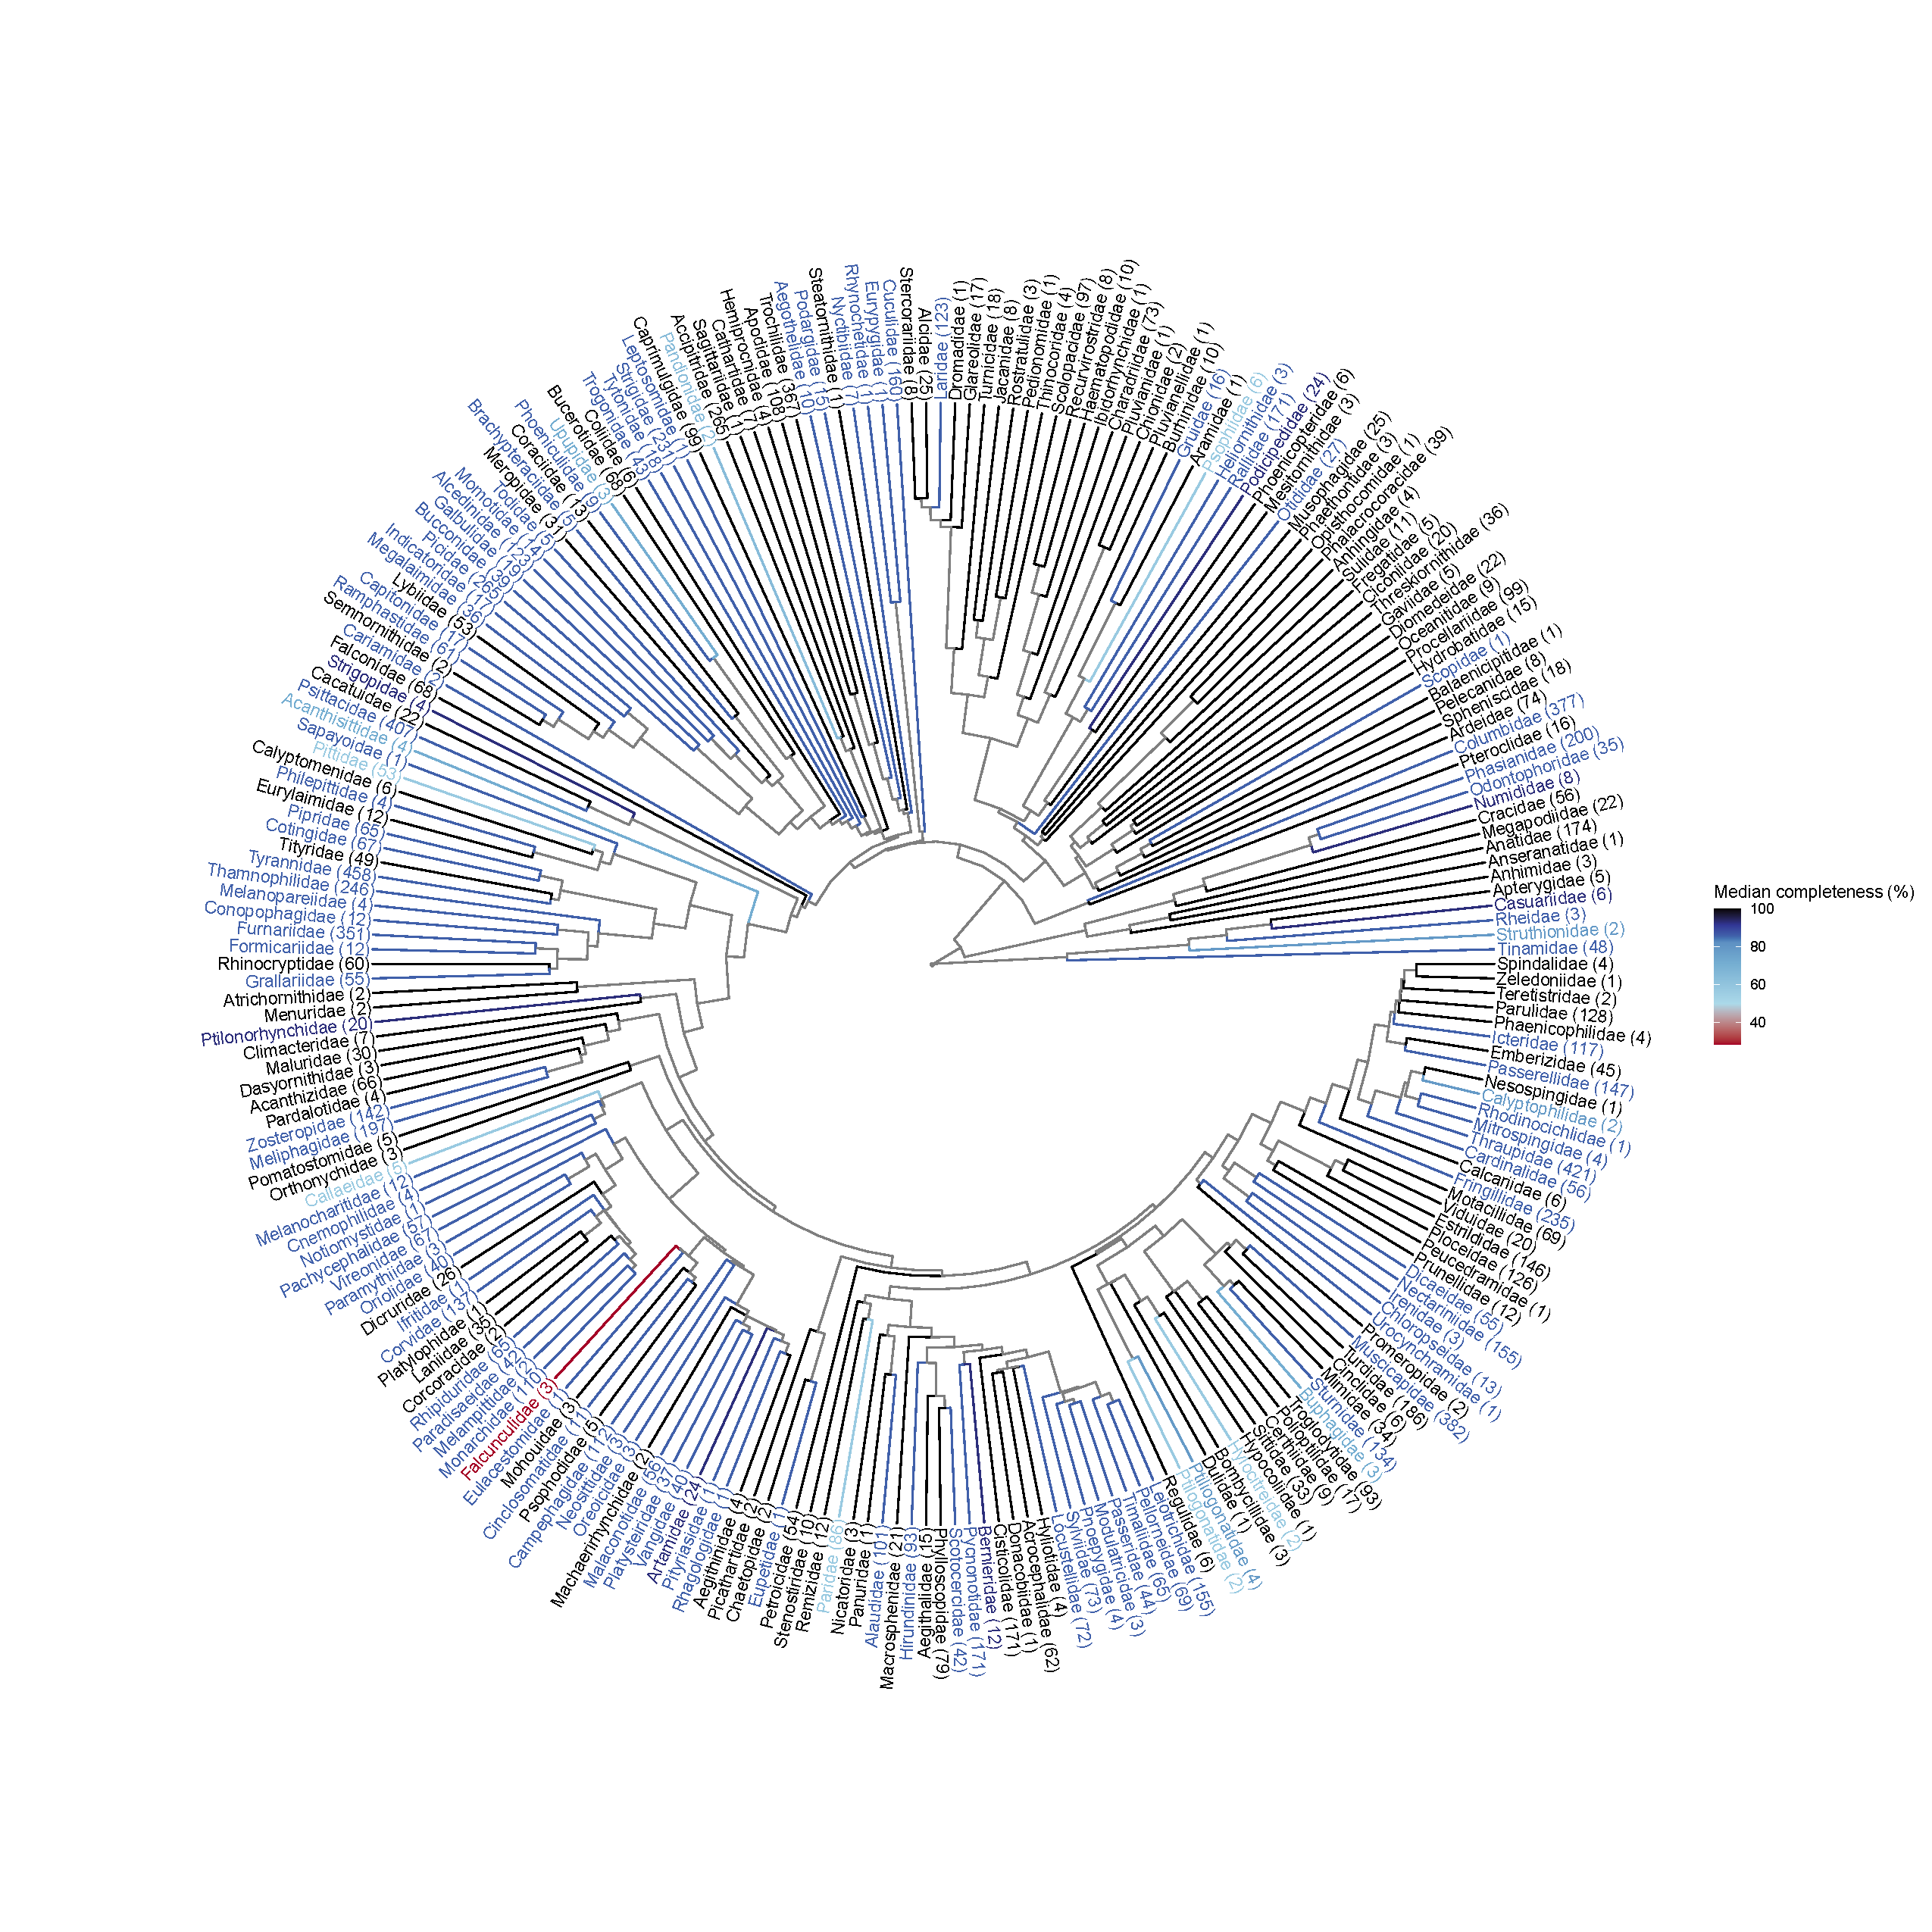
\includegraphics[scale=0.5,clip, trim=100 100 0 160]{Supporting/Chapter2/Figures/Phylogenies/Circular_birds_V2}
\caption[Within-family median trait completeness in birds]{\textbf{Within-family median trait completeness in birds.}}
\label{}
\end{figure}

\end{landscape}


\newpage
\pagebreak

\begin{figure}[]
\centering
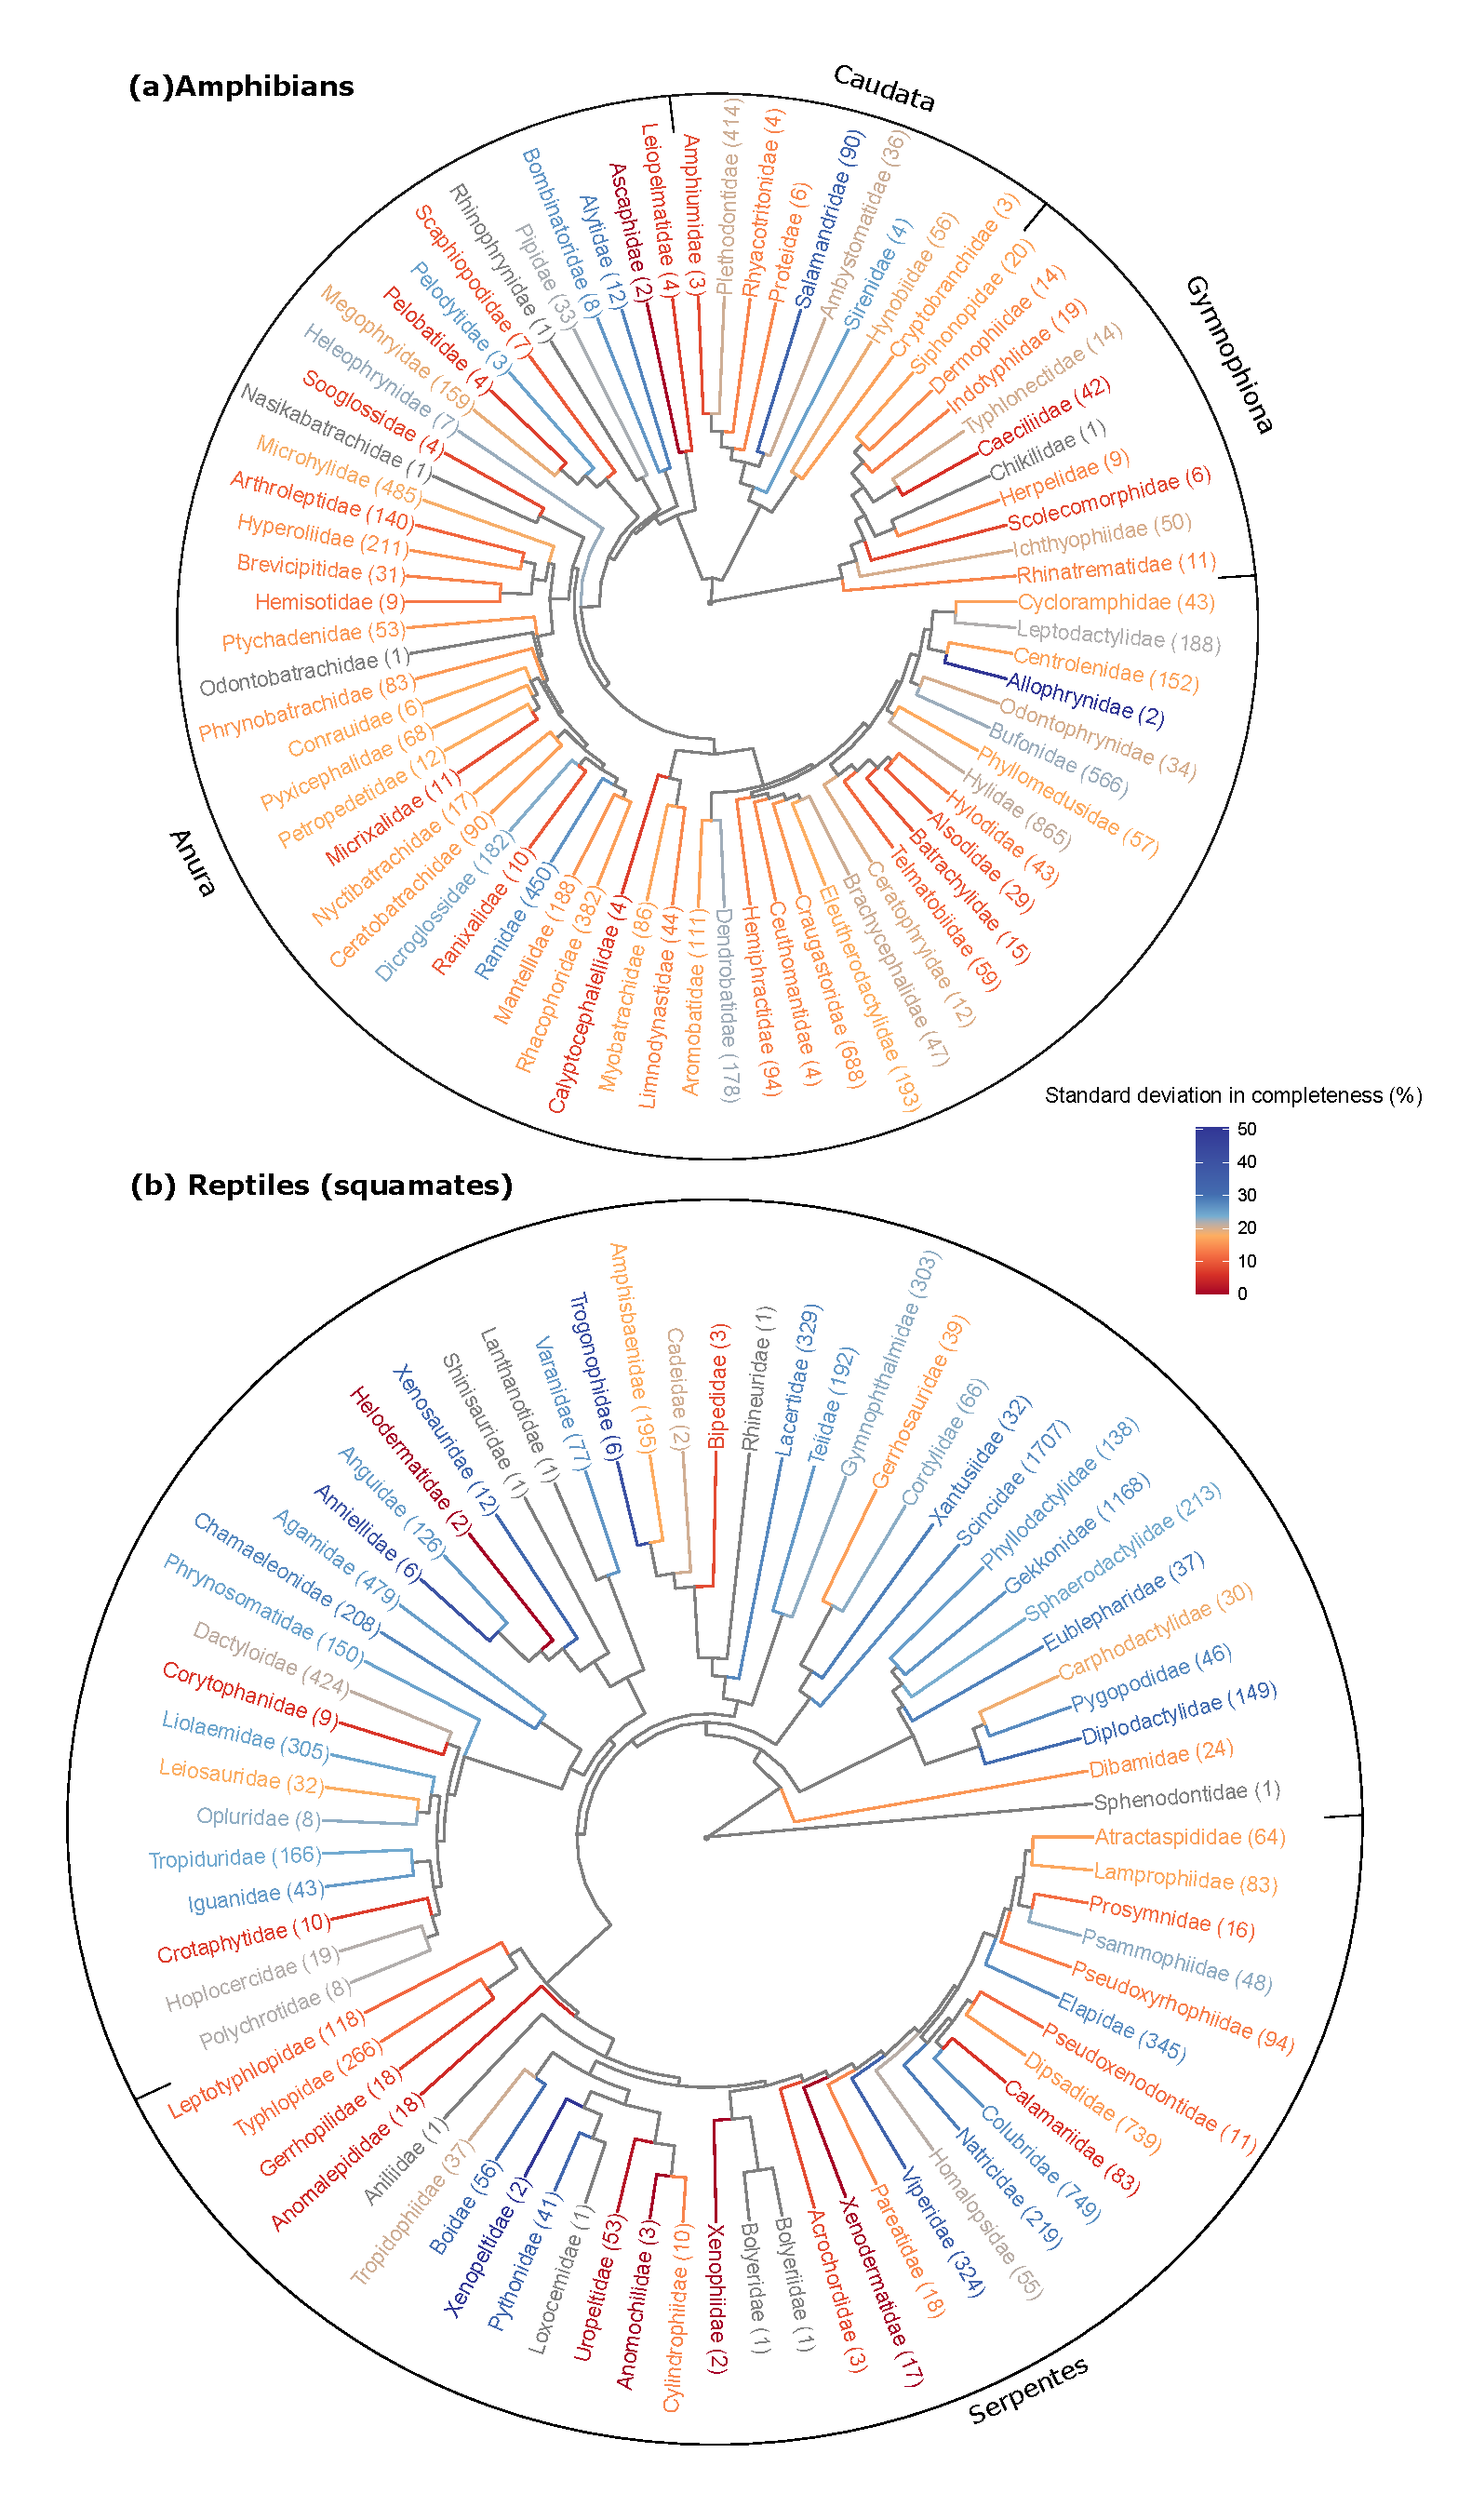
\includegraphics[scale=0.5, clip, trim=0 0 0 0]{Supporting/Chapter2/Figures/Phylogenies/Circular_herptiles_SD}
\caption[Within-family standard deviation in completeness.]{\textbf{Within-family standard deviation in completeness (herptiles).}}
\label{}
\end{figure}

\newpage
\pagebreak

\begin{figure}[h]
\centering
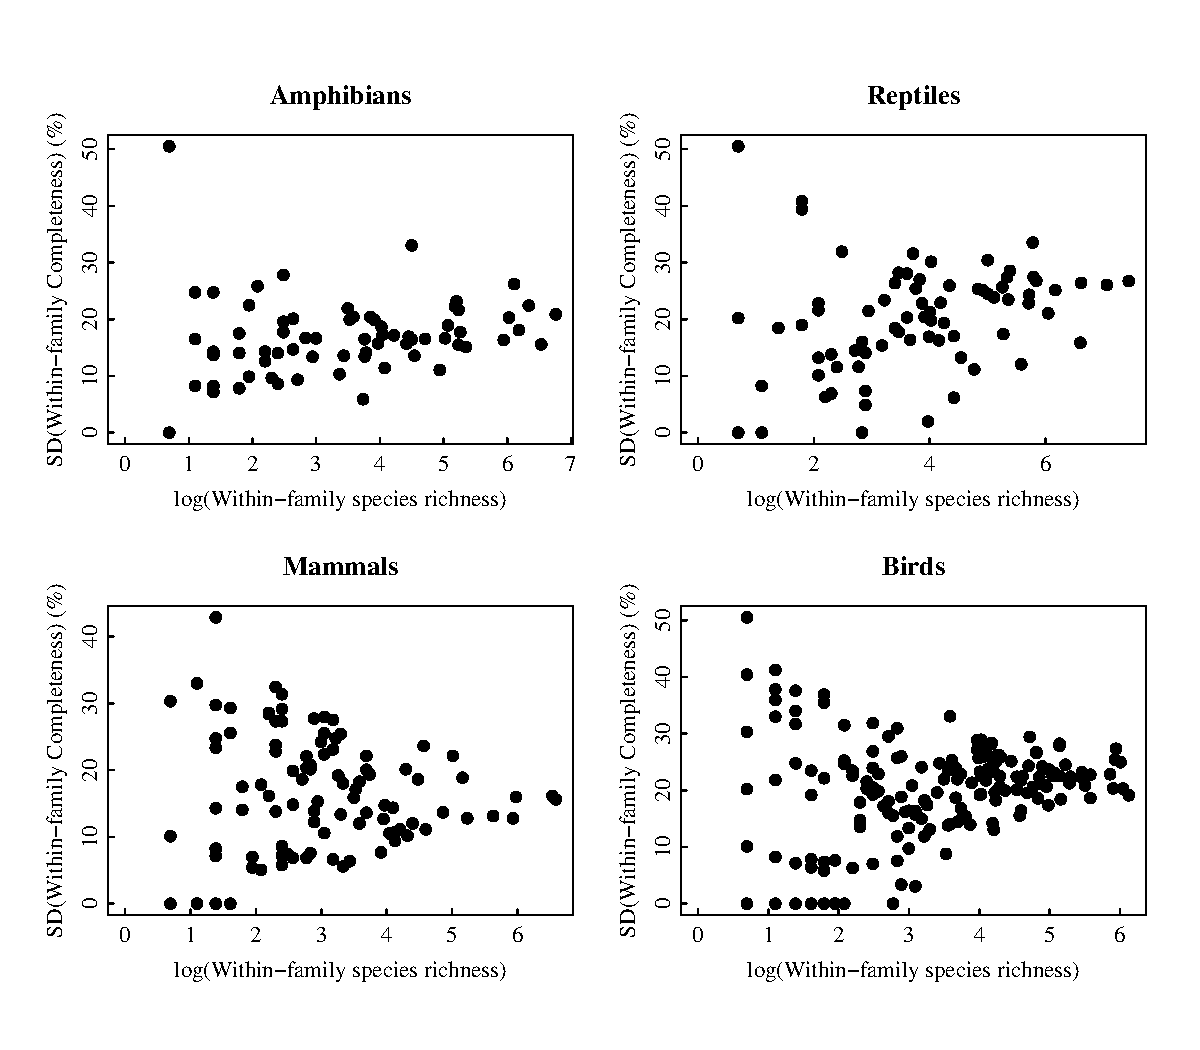
\includegraphics[scale=.6]{Supporting/Chapter2/Figures/Phylogenies/SD_VS_SR}
\caption[]{\textbf{Within-family species richness against the within-family standard deviation of completeness.}}
\label{}
\end{figure}

\clearpage
\section{Model coefficients for Range size against Number of sampled traits (Poisson model).}

%% New model coefficients:
\begin{table}[!htbp] \centering 
  \caption{\textbf{Coefficients of the model investigating whether species range size explained the number of sampled traits.} Class was added as an interacting predictor. The reference level for class is Mammals. The model was fitted using Poisson error distribution.} 
  \label{} 
\begin{tabular}{@{\extracolsep{5pt}} ccccc} 
\\[-1.8ex]\hline 
\hline \\[-1.8ex] 
 & Estimate & Std. Error & z value & Pr(\textgreater \textbar z\textbar ) \\ 
\hline \\[-1.8ex] 
Intercept & $1.678$ & $0.022$ & $76.809$ & $< 2e-16$ \\ 
log Range Size & $0.015$ & $0.002$ & $8.086$ & $6.16e-16$ \\ 
Class Birds & $$-$0.092$ & $0.028$ & $$-$3.350$ & $ 0.000809$ \\ 
Class Amphibians & $$-$0.689$ & $0.029$ & $$-$24.099$ & $< 2e-16$ \\ 
Class Reptiles & $$-$0.872$ & $0.027$ & $$-$31.856$ & $< 2e-16$ \\ 
log Range Size:Class Birds & $0.003$ & $0.002$ & $1.415$ & $0.157$ \\ 
log Range Size:Class Amphibians & $0.017$ & $0.003$ & $6.427$ & $ 1.30e-10$ \\ 
log Range Size:Class Reptiles & $0.026$ & $0.002$ & $11.159$ & $< 2e-16$ \\ 
\hline \\[-1.8ex] 
\end{tabular} 
\end{table}


\clearpage

\begin{table}[!htbp] \centering 
  \caption{\textbf{Coefficients of the model investigating whether species range size explained the number of sampled traits, \textit{using range maps not cut by altitudinal limits.}} Class was added as an interacting predictor. The reference level for class is Mammals. The model was fitted using Poisson error distribution.} 
  \label{} 
\begin{tabular}{@{\extracolsep{5pt}} ccccc} 
\\[-1.8ex]\hline 
\hline \\[-1.8ex] 
 & Estimate & Std. Error & z value & Pr(\textgreater \textbar z\textbar ) \\ 
\hline \\[-1.8ex] 
Intercept & $1.665$ & $0.023$ & $72.070$ & $< 2e-16$ \\ 
log Range Size & $0.015$ & $0.002$ & $8.167$ & $3.16e-16$ \\ 
Class Birds & $$-$0.110$ & $0.029$ & $$-$3.763$ & $0.0002$ \\ 
Class Amphibians & $$-$0.700$ & $0.030$ & $$-$23.721$ & $< 2e-16$ \\ 
Class Reptiles & $$-$0.928$ & $0.029$ & $$-$32.403$ & $< 2e-16$ \\ 
log Range Size:Class Birds & $0.004$ & $0.002$ & $1.840$ & $0.066$ \\ 
log Range Size:Class Amphibians & $0.018$ & $0.003$ & $6.564$ & $5.24e-11$ \\ 
log Range Size:Class Reptiles & $0.031$ & $0.002$ & $12.630$ & $< 2e-16$ \\ 
\hline \\[-1.8ex] 
\end{tabular} 
\end{table} 

\begin{figure}[h!]
\centering
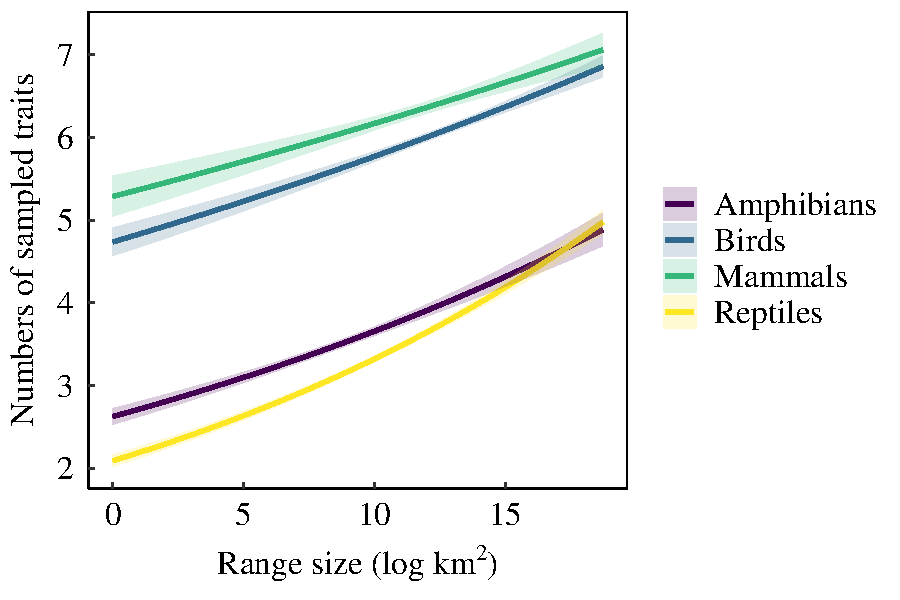
\includegraphics[scale=0.7]{Supporting/Chapter2/Figures/Plot_BeforeCuttingRS}
\caption[Relationship between number of sampled traits and geographical range size using distribution maps not cut by altitudina limits.]{\textbf{Relationship between number of sampled traits and geographical range size \textit{using distribution maps not cut by altitudinal limits}.} Models were fitted using a Poisson error distribution. Class was added as a predictor interacting with range size. Rates of increase were not significantly different for mammals and birds, but differed for reptiles and amphibians, with steeper rates of increase for reptiles overall. Cutting range maps by altitudinal limits had little effects on the results (Figure 4 in Main text).} 
\label{}
\end{figure}


\newpage
\pagebreak
\clearpage



% sample for spatial analyses
\section{Spatial models summaries}

% model summaries - amphibians
  \begin{table}[!htbp] \centering 
  \caption{Spatial model summary for amphibians. The spatial model was fitted to explain assemblage-level median completeness with species richness. Biogeographic realm was added as an interacting explanatory variable.} 
  \label{} 
\begin{tabular}{@{\extracolsep{5pt}} ccccc} 
\\[-1.8ex]\hline 
\hline \\[-1.8ex] 
 & Estimate & Std. Error & z value & Pr(\textgreater \textbar z\textbar ) \\ 
\hline \\[-1.8ex] Intercept - Realm: Afrotropic & $0.0738$ & $0.0064$ & $11.4908$ & $0$ \\ 
log(Species richness) & $$-$0.0025$ & $0.0017$ & $$-$1.4261$ & $0.1538$ \\ 
Realm: Australasia & $$-$0.0109$ & $0.0095$ & $$-$1.1453$ & $0.2521$ \\ 
Realm: Indo-Malay & $0.0455$ & $0.0119$ & $3.8294$ & $0.0001$ \\ 
Realm: Nearctic & $0.0441$ & $0.0082$ & $5.3905$ & $0.000000$ \\ 
Realm: Neotropic & $$-$0.0377$ & $0.0083$ & $$-$4.5538$ & $0.00001$ \\ 
Realm: Palearctic & $0.0047$ & $0.0067$ & $0.6992$ & $0.4844$ \\ 
log(Species richness):Australasia & $0.0018$ & $0.0038$ & $0.4789$ & $0.6320$ \\ 
log(Species richness):Indo-Malay & $$-$0.0147$ & $0.0039$ & $$-$3.7294$ & $0.0002$ \\ 
log(Species richness):Nearctic & $$-$0.0097$ & $0.0030$ & $$-$3.2003$ & $0.0014$ \\ 
log(Species richness):Neotropic & $0.0144$ & $0.0026$ & $5.6454$ & $0.000000$ \\ 
log(Species richness):Palearctic & $0.0109$ & $0.0029$ & $3.7358$ & $0.0002$ \\ 
\hline \\[-1.8ex] 
\end{tabular}  
\end{table} 

% model summary - reptiles
\begin{table}[!htbp] \centering 
  \caption{Spatial model summary for reptiles. The spatial model was fitted to explain assemblage-level median completeness with species richness. Biogeographic realm was added as an interacting explanatory variable.} 
  \label{} 
\begin{tabular}{@{\extracolsep{5pt}} ccccc} 
\\[-1.8ex]\hline 
\hline \\[-1.8ex] 
 & Estimate & Std. Error & z value & Pr(\textgreater \textbar z\textbar ) \\ 
\hline \\[-1.8ex] 
Intercept - Realm: Afrotropic & $0.2001$ & $0.0144$ & $13.9349$ & $0$ \\ 
log(Species richness) & $$-$0.0316$ & $0.0031$ & $$-$10.0547$ & $0$ \\ 
Realm: Australasia & $$-$0.1284$ & $0.0189$ & $$-$6.7851$ & $0$ \\ 
Realm: Indo-Malay & $$-$0.0453$ & $0.0263$ & $$-$1.7215$ & $0.0852$ \\ 
Realm: Neartic & $$-$0.0788$ & $0.0140$ & $$-$5.6366$ & $0.000000$ \\ 
Realm: Neotropic & $$-$0.0932$ & $0.0145$ & $$-$6.4425$ & $0$ \\ 
Realm: Palearctic & $$-$0.1030$ & $0.0131$ & $$-$7.8787$ & $0$ \\ 
log(Species richness):Australasia & $0.0386$ & $0.0046$ & $8.4019$ & $0$ \\ 
log(Species richness):Indo-Malay & $0.0124$ & $0.0061$ & $2.0397$ & $0.0414$ \\ 
log(Species richness):Neartic & $0.0346$ & $0.0038$ & $9.1601$ & $0$ \\ 
log(Species richness):Neotropic & $0.0220$ & $0.0034$ & $6.4231$ & $0$ \\ 
log(Species richness):Palearctic & $0.0286$ & $0.0033$ & $8.6153$ & $0$ \\ 
\hline \\[-1.8ex] 
\end{tabular}  
\end{table} 

\newpage
\pagebreak

\section{Trait coverage and taxonomic matching}

Here, we briefly explore the robustness of our work to taxonomic uncertainty by comparing trait coverage obtained with our procedure for taxonomic matching against trait coverage obtained when extracting synonyms from class-specific sources, which could contain more information, notably for herptiles. We aligned taxonomy again using the rangeBuilder R package, which allows the extraction of accepted names from class-specific sources. Overall, our results are robust to the use of different taxonomic backbones; the main conclusions are likely to be unaffected by taxonomic uncertainty.

\begin{figure}[h!]
\centering
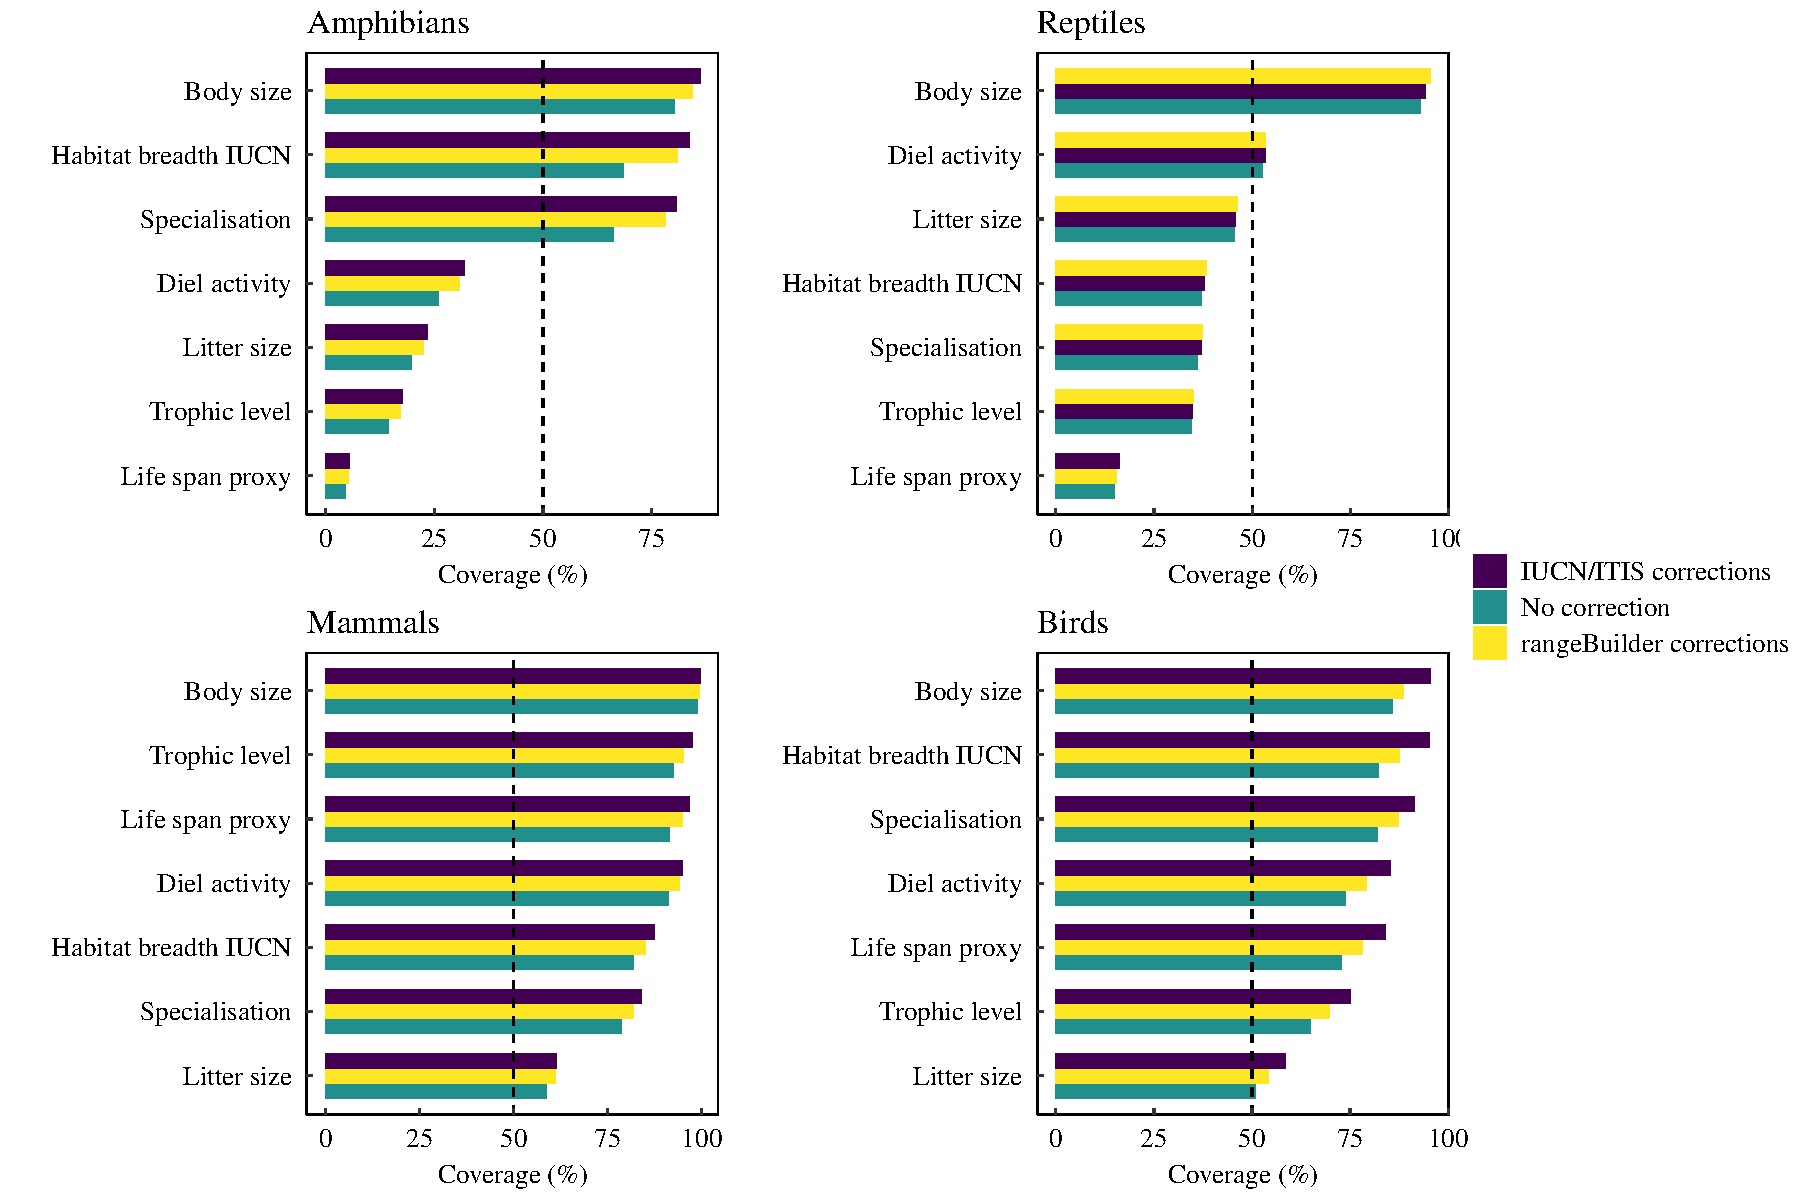
\includegraphics[scale=0.6]{Supporting/Chapter2/Figures/Coverage/DeltaCov_F3}
\caption[]{\textbf{Comparison of trait coverage among datasets corrected for taxonomy using the described procedure (purple bars), datasets corrected using the rangeBuilder package (extraction of synonyms from class-specific sources, yellow bars) and datasets where no taxonomic correction was applied when matching sources (green bars).}}
\label{}
\end{figure}

\addcontentsline{toc}{chapter}{Appendix 3: Supporting information for Chapter 3}
\chapter*{Appendix 3: Supporting information for Chapter 3}

\addcontentsline{toc}{chapter}{Appendix 4: Supporting information for Chapter 4}
\chapter*{Appendix 4: Supporting information for Chapter 4}



\end{document}